%% Working master-thesis draft assembled from the TUM SPS template.
\documentclass[
  a4paper,
  thesis=student,
  english,
  coverpage=false,
  titlepage=false,
  oneside,
  headmarks=true
]{tumbook}

\usepackage[utf8]{inputenc}
\usepackage[T1]{fontenc}
\usepackage{microtype}
\usepackage{booktabs}
\usepackage{longtable}
\usepackage{tabularx}
\usepackage{array}
\usepackage{multirow}
\usepackage{threeparttable}
\usepackage{graphicx}
\usepackage{float}
\usepackage{subcaption}
\usepackage{placeins}
\usepackage{amsmath,amssymb}
\usepackage{siunitx}
\usepackage{enumitem}
\usepackage{xcolor}
\usepackage{listings}
\usepackage{url}
\usepackage{csquotes}
\usepackage{natbib}
\usepackage{tikz}
\usepackage[acronym,toc,nonumberlist]{glossaries}
\makenoidxglossaries
\loadglsentries{chapters/glossary.tex}

% Institutional identity for the TUM SPS thesis template.
\AtBeginDocument{%
  \renewcommand{\theChairName}{Chair of Spacecraft Systems}%
  \renewcommand{\theDepartmentName}{TUM School of Engineering and Design}%
}

% TeX Gyre Heros is metric-compatible with Helvetica and supplies the full
% regular/bold/italic font set required by portable Tectonic builds.
\usepackage{tgheros}
\renewcommand{\sfdefault}{qhv}
\renewcommand{\familydefault}{\sfdefault}

\graphicspath{{figures/}{figures/nominal/}{figures/california_v2/}{figures/objective_weights/}}
\hypersetup{
  colorlinks=true,
  linkcolor=TUMBlue,
  citecolor=TUMBlue,
  urlcolor=TUMBlue,
  pdftitle={Effect of Central Nodes on Task Allocation in Distributed Satellite Systems for Wildfire Detection},
  pdfauthor={Maneesh Manjunath}
}

\sisetup{detect-all,round-mode=places,round-precision=2}
\setlist{itemsep=0.25em,topsep=0.4em}
\setlength{\emergencystretch}{2em}
\clubpenalty=10000
\widowpenalty=10000
\displaywidowpenalty=10000

\newcolumntype{Y}{>{\raggedright\arraybackslash}X}
\newcolumntype{L}[1]{>{\raggedright\arraybackslash}p{#1}}
\newcolumntype{C}[1]{>{\centering\arraybackslash}p{#1}}
\newcommand{\todo}[1]{\textcolor{red!80!black}{\textbf{Open item:} #1}}
\newcommand{\workingdraft}{\textcolor{orange!75!black}{\textbf{Working draft}}}
\newcommand{\codeverified}{\textcolor{green!45!black}{\textbf{Validated result}}}
\newcommand{\inprogress}{\textcolor{orange!75!black}{\textbf{In progress}}}
\newcommand{\notclaimed}{\textcolor{red!65!black}{\textbf{Not claimed}}}
\newcommand{\metric}[1]{\ensuremath{\mathrm{#1}}}
\newcommand{\Suseful}{\ensuremath{S_{100}^{\mathrm{useful}}}}
\newcommand{\sourcepath}[1]{\texttt{\detokenize{#1}}}
\newcommand{\pendingresult}[1]{%
  \begin{center}\fcolorbox{orange!70!black}{orange!5}{%
  \begin{minipage}{0.90\textwidth}\textbf{Result pending.} #1\end{minipage}}\end{center}}
\newcommand{\evidencebox}[2]{%
  \begin{center}\fcolorbox{TUMBlue}{TUMBlue!4}{%
  \begin{minipage}{0.90\textwidth}\textbf{#1} #2\end{minipage}}\end{center}}

\lstset{
  basicstyle=\ttfamily\small,
  breaklines=true,
  frame=single,
  columns=fullflexible,
  keepspaces=true,
  showstringspaces=false
}


\title{Effect of Central Nodes on Task Allocation in Distributed Satellite Systems for Wildfire Detection}
\subtitle{Communication-Constrained Dissemination, Follow-Up Observation, and Architecture Trade-Space Analysis}
\author{Maneesh Manjunath}
\degree{Master of Science (M.Sc.)}
\dateSubmitted{Working draft, 2 September 2026}
\examiner{To be confirmed}
\supervisor{Vincenzo Messina}

\begin{document}
\frontmatter
\maketitle

\chapter{Draft Status and Reading Guide}
\workingdraft\ for supervisor review, updated on 2 September 2026. This version integrates every locally available validated evidence layer while keeping unfinished work visible. It is not a submission copy.

The report uses two related campaigns that must not be numerically merged:
\begin{enumerate}
\item the validated two-region nominal campaign, containing 891 Walker/CN cases for California and 891 for India, is retained for the regional comparison and the historical nominal trade-space result; and
\item the newer \textit{Full891 Fresh V2} campaign, containing 539 scenario definitions per architecture case, is the authoritative source for the updated simulator, California policy ablation, controlled task-size experiments, injected failures, and revised objective-weight analysis.
\end{enumerate}

The California Fresh V2 archive contains all 891 architecture identifiers. A total of 890 cases have complete success markers. The remaining case, \path{T180_P10_H1000_I0986_CN100_F1}, contains 400 of 539 expected scenario rows and is excluded from comparisons that require a complete scenario set. After removing 4,269 resume duplicates, 480,110 unique scenario rows remain. All 19,179 recorded architecture-validation checks pass and no completed scientific row has status \texttt{FAILED}.

No completed India Fresh V2 archive was found in the accessible project data at the time of this update. India-specific robustness and controlled-sensitivity values are therefore not inferred from California or from the earlier nominal campaign. The existing two-region nominal results remain identified as a separate evidence layer. Observation-radius sensitivity has not been executed, and Fresh V2 does not retain a separately named first-reception-latency metric in its canonical case table; these limitations are stated wherever they affect a research question.

The official submission date, examiner, declaration, and final repository release tag remain administrative open items. The source and compiled PDF in this repository are intended for transparent supervisor review and automated checking.

\chapter{Zusammenfassung}
Verteilte Satellitensysteme k"onnen zeitkritische Erdbeobachtungsaufgaben schneller bearbeiten, ihre Leistungsf"ahigkeit h"angt jedoch von orbitalem Zugang, begrenzten Kommunikationsfenstern und der gew"ahlten Weiterleitungsstrategie ab. Diese Arbeit untersucht den Einfluss eines Zentralenknotenanteils auf die Verteilung von Waldbrandaufgaben, die nachfolgende Beobachtung, den Ressourcenbedarf und die Empfindlichkeit gegen Ausf"alle. Eine nachvollziehbare Datenpipeline erzeugt aus deduplizierten Sentinel-3-SLSTR-FRP-Detektionen 805 priorisierte Aufgaben: 32 f"ur Kalifornien und 773 f"ur Indien.

Der Entwurfsraum umfasst 60, 120 und 180 Satelliten, 3, 5 und 10 Bahnebenen, H"ohen von 500, 800 und 1000 km, Inklinationen von 60, 80 und 98,6 Grad sowie Zentralenknotenanteile zwischen 0 und 100 Prozent. Die fr"uhere nominale Kampagne enth"alt 891 validierte F"alle pro Region. Die neuere Full891-Fresh-V2-Kampagne definiert 539 Betriebs-, Policy-, Aufgabengr"o\ss en- und Fehlerszenarien pro Architektur. F"ur Kalifornien liegen 890 vollst"andige F"alle und nach Entfernung von Resume-Duplikaten 480.110 eindeutige Szenariozeilen vor; alle 19.179 Architekturpr"ufungen wurden bestanden.

In der begrenzten nominalen Policy betr"agt die mittlere Beobachtungserf"ullung 61,59 Prozent, die strikte vollst"andige Verteilung an n"utzliche Empf"anger 0,63 Prozent und deren mittlere Abdeckung 15,29 Prozent. Das diagnostische Szenario ohne Hop- und Kopienbegrenzung erh"oht diese Werte auf 77,62, 74,69 und 91,14 Prozent, steigert jedoch die mittlere "ubertragene Datenmenge von 197,55 auf 2.047,57 Mbit pro Fall. Die Wirkung des Zentralenknotenanteils ist nicht monoton und zeigt abnehmenden Grenznutzen bei weiter wachsender Kommunikationslast.

Bei einem Stressniveau von 30 Prozent ist der Ausfall der einzigen Bodenstation die dominante kalifornische Schwachstelle. Eine Vervierfachung der Aufgabengr"o\ss e reduziert die mittlere Beobachtungserf"ullung von 77,62 auf 69,48 Prozent. Eine Pareto-konsistente Gewichtungsanalyse bevorzugt bei ausgewogenen Annahmen eine Konfiguration mit 60 Satelliten, 10 Ebenen, 800 km H"ohe, 98,6 Grad Inklination und 40 Prozent Zentralenknoten. Diese Konfiguration gewinnt 41,79 Prozent von 10.000 zuf"alligen Gewichtungsziehungen. Das Ergebnis ist ein bedingter Kompromiss und kein universelles Optimum. Die Indien-Fresh-V2-Ergebnisse und eine Sensitivit"at des Beobachtungsradius bleiben vor der abschlie\ss enden regions"ubergreifenden Robustheitsaussage offen.

\chapter{Abstract}
Distributed satellite systems can shorten the response to time-critical Earth-observation events, but their performance depends on orbital access, finite communication opportunities, and the routing policy used to disseminate tasks. This thesis studies how assigning a fraction of a Walker constellation to a central-node communication and routing role affects wildfire-task dissemination, follow-up observation, resource demand, and failure sensitivity. A traceable preprocessing pipeline converts de-duplicated Sentinel-3 SLSTR fire-radiative-power detections into 805 prioritized tasks: 32 for California and 773 for India. Each task retains a release time, location, priority-dependent data volume, deadline, and source provenance.

The architecture grid combines 60, 120, and 180 satellites; 3, 5, and 10 planes; altitudes of 500, 800, and 1000 km; inclinations of 60, 80, and 98.6 degrees; and central-node fractions from 0 to 100 percent. The earlier nominal campaign contains 891 validated cases per region and establishes that architecture preferences are region- and metric-dependent. The newer Full891 Fresh V2 campaign evaluates 539 operational, policy, task-size, and failure scenarios per architecture. The locally available California archive contains 890 complete cases and 480,110 unique case-scenario rows after resume de-duplication; all 19,179 architecture checks pass.

For California Fresh V2, the bounded nominal policy achieves mean observation fulfilment of 61.59 percent, strict useful-recipient dissemination of 0.63 percent, and useful-recipient coverage of 15.29 percent. Removing hop and copy restrictions in the \texttt{unlimited\_useful\_deadline} diagnostic increases these means to 77.62, 74.69, and 91.14 percent, at the cost of increasing transferred data from 197.55 to 2,047.57 Mbit per case. Under the nominal policy, observation fulfilment is non-monotonic: it reaches 71.13 percent at 50 percent central nodes in the balanced subset and falls to 35.70 percent at 100 percent. Under the unlimited diagnostic, dissemination saturates while communication burden continues to rise.

At a 30 percent stress level, ground-station outage is the dominant California vulnerability, reducing observation and strict dissemination by 21.46 and 20.84 percentage points on average. Random satellite and central-node failures produce smaller mean losses, while capacity degradation has limited average effect. Increasing task size from one to four times the nominal value reduces mean observation fulfilment from 77.62 to 69.48 percent and strict dissemination from 74.69 to 60.10 percent. A Pareto-consistent objective-weight analysis selects a 60-satellite, 10-plane, 800 km, 98.6-degree, 40-percent-central-node configuration for balanced and performance-dominant preferences; it wins 41.79 percent of 10,000 randomized preference draws. This is a conditional compromise, not a universal optimum. India Fresh V2 and observation-radius sensitivity remain required before the final cross-region robustness conclusion.

\chapter{Acknowledgements}
I thank Vincenzo Messina for providing the communication model, facilitating the use of TAT-C, and guiding the development of the research questions and evaluation requirements. I am grateful to the Chair of Spacecraft Systems at the Technical University of Munich for the academic environment in which this work was conducted.

The wildfire-data pipeline, integration code, campaign automation, post-processing, analysis, and report preparation were carried out by the author. The communication model and the TAT-C basis were provided by Vincenzo Messina and are identified as such in the methodology and contribution statement. This wording should be reviewed before the final submission together with the official authorship and software-licensing statements.



\tableofcontents
\listoffigures
\addcontentsline{toc}{chapter}{List of Figures}
\listoftables
\addcontentsline{toc}{chapter}{List of Tables}
\glsaddall
\printnoidxglossaries

\mainmatter
\chapter{Introduction}
\section{Motivation}

Earth-observation missions are moving from isolated spacecraft operations toward constellations in which sensing, communication, and decision-making are distributed across many nodes. This transition creates two coupled design problems. The first is geometric: a spacecraft must obtain access to a target at an operationally useful time. The second is informational: the task describing that target must reach a suitable spacecraft early enough for the access to be used. A constellation with excellent coverage can therefore fail a time-critical mission if the task is disseminated too late, while a well-connected network cannot observe an event for which no suitable access exists.

Wildfire response makes this coupling visible. A remote-sensing product may indicate a new or growing fire, but the detection alone is not the end of the operational chain. The event must be transformed into a task, prioritized, released into the network, forwarded within finite communication opportunities, received by one or more candidate observers, and finally executed before a response deadline. A useful performance evaluation must preserve this event order. It must also distinguish the time to first reception, the breadth of dissemination, and the completion of a follow-up observation.

One way to improve coordination is to assign selected spacecraft a central-node role. Conceptually, a central node may have additional processing, storage, cross-link capability, routing responsibility, coordination authority, or connectivity to ground. Such a node can accelerate information exchange, but it can also increase hardware differentiation and create operational dependencies. The design question is therefore not simply whether central nodes help. It is whether a particular degree of centralization improves mission fulfilment sufficiently to justify the added resource burden and the possible loss of robustness.

This thesis investigates that question through a full-factorial Walker-constellation campaign driven by real, de-duplicated Sentinel-3 wildfire tasks. The implemented experiment varies the fraction of satellites labelled as central nodes while also varying constellation size, plane count, altitude, and inclination. The result is a controlled architecture database in which communication, reception, observation, and resource metrics can be evaluated together.

\section{Problem Statement}

The starting task-allocation logic was developed for a different Earth-observation application. Adapting it to wildfire detection required more than changing the target coordinates. The wildfire use case introduces multiple simultaneous events, unequal priority, priority-dependent deadlines, priority-dependent task sizes, region-specific task density, and the need to validate tasks against physical fire observations. It also requires the simulator to distinguish dissemination from observation fulfilment.

The central problem addressed by this work is stated as follows:

\begin{quote}
Given a time-stamped set of prioritized wildfire tasks, a Walker observer constellation, a ground-station configuration, finite communication opportunities, and a configurable fraction of central nodes, determine how architecture and centralization affect task reception, dissemination breadth, follow-up observation, communication burden, and decision robustness.
\end{quote}

The phrase \emph{decision robustness} is used for stability under objective weights. Physical robustness refers separately to the retention of mission performance after injected node failures. Keeping those two meanings separate prevents a stable ranking from being mistaken for a failure-tolerant architecture.

\section{Aim and Objectives}

The aim is to establish a defensible performance--resource--robustness trade space for wildfire task allocation in a distributed satellite system. The objectives are:

\begin{enumerate}
\item construct a traceable wildfire-task dataset from Sentinel-3 SLSTR FRP products, supported by FIRMS screening and event validation;
\item adapt the task-allocation framework to multiple release times, priority classes, task sizes, and deadlines;
\item model finite, time-dependent communication windows and evaluate observation only after task reception;
\item execute and validate the complete 891-case Walker and central-node design grid for two event regions and the expanded 539-scenario Fresh V2 campaign where available;
\item quantify central-node, orbit, constellation-size, communication-load, and regional effects without assigning causal meaning to unadjusted correlations;
\item identify exact Pareto sets and evaluate the stability of architecture rankings under alternative objective weights; and
\item quantify robustness through explicit random and targeted node-removal, link-window, ground-station, and capacity-degradation experiments rather than through nominal failure labels.
\end{enumerate}

Table~\ref{tab:objective_evidence} maps each objective to the evidence used in this draft. The two-region nominal layer is complete. Fresh V2 robustness, task-size, policy, and revised weight analyses are complete for California; the corresponding India Fresh V2 extension is not locally available and is not inferred.

\begin{table}[htbp]
\centering
\small
\caption{Objectives, evidence products, and status in this working draft.}
\label{tab:objective_evidence}
\begin{tabularx}{\textwidth}{L{0.07\textwidth}Y L{0.28\textwidth} L{0.17\textwidth}}
\toprule
No. & Objective & Primary evidence & Status \\
\midrule
O1 & Sentinel-3 wildfire task construction & De-duplicated 805-task CSV and processing history & Complete \\
O2 & Multi-task priority and deadline model & Case-level \path{wildfire_tasks_used.csv} & Complete \\
O3 & Capacity-aware dissemination and observation-after-reception & Windows, transfers, receptions, and observation results & Complete \\
O4 & Full architecture campaign & 1,782 earlier nominal cases; California Fresh V2 scenario archive & Nominal complete; Fresh V2 California complete \\
O5 & Architecture and regional effects & Earlier paired-region tables and Fresh V2 California factor effects & Partial for final V2 regional comparison \\
O6 & Pareto and weight sensitivity & Exact Pareto membership and 10,000 revised weight draws & Complete for Fresh V2 California \\
O7 & Failure-injection robustness & Random/targeted failures, outages, and capacity degradation & Complete for Fresh V2 California \\
\bottomrule
\end{tabularx}
\end{table}

\section{Research Questions}

The approved questions are made operational through the exported metrics:

\begin{enumerate}[label=RQ\arabic*.,leftmargin=*]
\item How can a PBL-focused distributed task-allocation framework be adapted to generate and process multiple time-critical wildfire tasks from real remote-sensing detections?
\item How do real wildfire task distributions, confidence values, fire intensity, and regional task density affect dissemination and observation fulfilment?
\item How does the fraction of central nodes influence first-reception latency, full dissemination, deadline success, observation fulfilment, routing depth, communication load, and architecture dependency?
\item Which Walker constellation configurations provide the best trade-off among performance, complexity, and robustness for wildfire monitoring?
\item How stable is the preferred central-node fraction under changes in task size, observation radius, failure mode, and objective-function weights?
\end{enumerate}

The available evidence answers RQ1 and the California-specific portions of RQ2--RQ5. Fresh V2 supplies validated California policy, task-size, failure, and weight experiments. A final Fresh V2 answer about regional load/generalization requires the India archive; observation-radius sensitivity and a separately extracted first-reception latency also remain open.

\section{Hypotheses}

Five hypotheses organize the analysis:

\begin{description}[leftmargin=3.5cm,style=nextline]
\item[H1: Diminishing returns] Increasing central-node fraction initially reduces dissemination latency and improves task fulfilment, but the marginal benefit diminishes after the network becomes sufficiently connected.
\item[H2: Resource penalty] Central-node count, communication opportunity, and dependency increase with centralization, so the fastest architecture need not be the preferred architecture.
\item[H3: Load dependence] A dense task region produces different capacity and ranking behaviour from a sparse event region even when the architecture grid is identical.
\item[H4: Geometry dependence] Successful reception is necessary but not sufficient for observation because a receiving satellite still needs a valid access before the deadline.
\item[H5: No universal optimum] The preferred case changes with region and objective weights; a defensible result is a Pareto set or stable candidate set rather than a universal scalar optimum.
\end{description}

\section{Scope and Boundaries}

Table~\ref{tab:scope_hierarchy_new} defines the scope hierarchy. Central-node fraction is the primary variable. Walker geometry supports the centrality analysis, while task size, observation radius, and node failure test the sensitivity of the main conclusion. A separate heterogeneous relay layer is outside the implemented nominal campaign.

\begin{table}[htbp]
\centering
\caption{Hierarchy of the implemented and planned thesis scope.}
\label{tab:scope_hierarchy_new}
\begin{tabularx}{\textwidth}{L{0.17\textwidth}L{0.31\textwidth}Y}
\toprule
Level & Study element & Treatment in this report \\
\midrule
Core & Central-node fraction in a wildfire DSS & Complete 0--100\% sweep for every base architecture \\
Supporting & Satellite count, plane count, altitude, inclination & Full-factorial nominal screening \\
Sensitivity & Objective weights & Complete 10,000-draw Fresh V2 California analysis \\
Sensitivity & Task size and injected failures & Complete for Fresh V2 California \\
Sensitivity & Observation radius & Fixed at 700 km; targeted sweep not executed \\
Extension & Dedicated heterogeneous central-node orbit & Conceptual discussion and future work only \\
Out of scope & Onboard fire-detection latency, weather, cloud, pointing, energy, and monetary cost & Explicitly excluded from final claims \\
\bottomrule
\end{tabularx}
\end{table}

The simulated mission chain starts when a processed wildfire task is injected. It does not simulate the original thermal measurement, onboard detection, cloud screening, product generation latency, or delivery of the final alert to civil-protection authorities. The observation radius is a mission-level access approximation and not a detailed optical-instrument pointing model. ``Cost'' means a declared non-monetary resource proxy; no procurement or lifecycle cost is inferred.

\section{Meaning of a Central Node}

The conceptual system definition and the implemented experiment are intentionally separated. Conceptually, central nodes may differ from ordinary satellites in hardware, processing, communication links, routing, coordination, and connection to ground. The final simulator represents only the portion for which validated code and outputs exist: selected nodes receive a central-node label, communication opportunities follow the configured link policy, and the routing policy preferentially forwards through the central-node structure. The campaign does not assign different sensor performance, processor speed, storage volume, reliability, or monetary cost to central nodes.

This distinction is essential for interpretation. A measured central-node effect is an effect of the implemented communication and routing role under common spacecraft geometry. It is not evidence that a particular hardware implementation is optimal. Hardware and operations can later be attached to the architectural role once real subsystem assumptions are available.

\section{Scientific and Engineering Contributions}

The thesis contributions are:

\begin{enumerate}
\item a real-data, de-duplicated Sentinel-3 task set that connects FRP, confidence, spatial clustering, priority, data size, and response deadline;
\item a modular DSS workflow separating physical communication and observation opportunities from the allocation/evaluation layer;
\item a capacity-aware and time-ordered forwarding evaluation that records task reception, transfer, observation, and failure evidence;
\item a complete two-region, 891-case-per-region nominal campaign plus a California Fresh V2 campaign with operational, policy, task-size, failure, and combined-stress scenarios;
\item a clear distinction between observation fulfilment, conditional reception latency, receiver coverage, and useful-recipient full dissemination;
\item exact Pareto filtering and Monte Carlo objective-weight sensitivity without claiming a universal optimum; and
\item reproducible random and targeted failure experiments with recorded seeds, separate original/surviving denominators, and time-aware mission metrics.
\end{enumerate}

The author developed the wildfire pipeline, integration, simulation automation, campaign execution, post-processing, statistical analysis, and report. Vincenzo Messina provided the communication model and the TAT-C basis. This allocation is stated here because the software components directly shape the interpretation of the results.

\section{Report Structure}

Chapter~2 presents the literature review. Chapter~3 explains the Sentinel-3 task dataset and de-duplication. Chapter~4 formalizes the Fresh V2 architecture, communication, routing, observation, and metrics. Chapter~5 separates the earlier two-region nominal evidence from the expanded Fresh V2 scenario design and validation. Chapter~6 reports the earlier validated regional baseline. Chapter~7 reports the available Fresh V2 California operational, policy, task-size, robustness, Pareto, and weight results. Chapter~8 answers the research questions with explicit evidence boundaries, while Chapter~9 gives the conclusions and remaining work. The appendices provide metric definitions, campaign configuration, validation records, supplementary tables, and software-release requirements.

\chapter{Background and Related Work}
\section{Distributed Satellite Systems}

A distributed satellite system (DSS) consists of multiple space assets that cooperate to achieve mission objectives that would otherwise be executed by an individual spacecraft or a centrally planned constellation. Distribution can occur across sensing, processing, communication, decision-making, and operations. The design space therefore spans tightly coordinated constellations, federated systems that share resources across mission owners, and autonomous networks that allocate observations onboard \citep{Golkar2015,Scrocciolani2024}. These categories should not be treated as interchangeable. A constellation describes an orbital and mission organization, whereas federation and decentralization describe how capabilities, information, and authority are shared.

Automation becomes increasingly important as the number of assets and requests grows. Reviews of large DSS operations identify a shift away from spacecraft-by-spacecraft commanding toward goal-based planning, automated monitoring, and coordination mechanisms that scale with the system rather than with the number of human operators \citep{BenLarbi2021}. This operational perspective is directly relevant to time-critical Earth observation: a constellation may have adequate geometric coverage, yet still respond too slowly if every new request must travel through a remote planning loop before any spacecraft can act.

Centralized coordination has two main advantages: global information can be combined into a coherent decision, and policy enforcement is comparatively simple. Its weaknesses are latency to the decision point, dependence on ground contact or a coordinating node, and scaling difficulty as task and asset counts increase. Fully decentralized coordination can improve local responsiveness and remove a single decision bottleneck, but may require repeated message exchange and may produce inconsistent local views under intermittent connectivity. Recent work consequently motivates decentralized satellite networking and onboard decision-making, while also recognizing the resulting coordination and protocol challenges \citep{Oh2024}.

Hybrid architectures occupy the space between these endpoints. Selected satellites can be assigned enhanced routing or coordination roles without making one node the permanent controller of the mission. This introduces an architectural design variable: how many enhanced nodes are needed, where they are placed, and what privileges they possess. A hybrid architecture is useful only when those privileges are explicit. Calling a satellite a ``central node'' does not itself improve performance; the effect must arise through defined link access, forwarding eligibility, processing capacity, storage, or coordination rules.

\section{Task Allocation and Observation Scheduling}

Earth-observation scheduling is a constrained resource-allocation problem involving target visibility, time windows, instrument constraints, task value, spacecraft resources, and communication opportunities \citep{Ferrari2025}. A planner must decide not only which requests are valuable but also whether a feasible sequence of observations exists. In a dynamic mission, new requests can arrive after a schedule has already been constructed, so the system must repeatedly trade schedule stability against responsiveness.

Large constellations make a single global optimization increasingly difficult to compute and communicate. Decentralized approaches partition the allocation problem across satellites, allowing agents to exchange local requests, bids, or partial schedules \citep{Parjan2023,Zilberstein2025}. Such methods can reduce dependence on a single planner and permit decisions nearer to the sensing assets. Their benefit, however, depends on the communication model: an allocation algorithm that assumes instantaneous exchange can look effective even when the corresponding messages could not reach the agents before the observation deadline.

It is therefore essential to distinguish decision quality from information availability. A scheduled observation and a disseminated task are different system states:

\begin{description}[leftmargin=4.2cm,style=nextline]
\item[Task generation] A wildfire event is converted into a request containing location, creation time, priority, deadline, and data-size assumptions.
\item[Task reception] A satellite has received sufficient task information to act on the request.
\item[Observation opportunity] Satellite geometry permits sensing the task location within the assumed field of regard or observation radius.
\item[Observation fulfilment] An opportunity occurs after reception and before the task deadline, and the observation is assigned or executed under the model.
\item[Data delivery] The resulting observation product is transferred to a ground station or another defined endpoint.
\end{description}

The separation exposes two different failure modes. A task can miss its deadline because no satellite has a suitable observation opportunity, even though dissemination was immediate. Conversely, a geometrically feasible opportunity can be lost because the task reached the observing satellite too late. Reporting only final observation success hides this distinction and makes it difficult to tell whether an architectural change improved coverage, communication, or both. For that reason, this thesis treats first reception, dissemination extent, observation fulfilment, and latency as separate metrics.

The present work focuses on dissemination of post-injection wildfire tasks and the subsequent observation opportunity. It does not simulate the complete chain from onboard thermal-anomaly detection through image-product downlink. Downlink latency studied in early baseline work remains useful context, but it cannot substitute for communication-aware task-reception metrics unless the mission boundary is explicitly extended.

\section{Time-Varying Satellite Connectivity}

Graph-based representations separate physical contact opportunities from the communication process. Let the time-dependent satellite network be
\begin{equation}
G(t) = \left(V,E(t)\right),
\end{equation}
where $V$ contains observer satellites, enhanced central nodes, and optionally ground stations, while $E(t)$ contains links available at time $t$. A contact window is a maximal interval over which a specific edge exists. A transfer event is an actual use of that edge to transmit a task. The distinction is important: a system may generate many windows but use only a small fraction of them, or repeatedly use a small number of bottleneck links.

A static snapshot cannot fully characterize such a network. Two nodes that are never connected by an instantaneous end-to-end path may still communicate over a temporal path if intermediate satellites store the task and forward it during later contacts. Delay- and disruption-tolerant networking formalizes this store--carry--forward behavior. Bundle Protocol version 7 is designed for stressed networks with intermittent connectivity and variable delay \citep{Burleigh2022}. For environments in which future contacts are predictable, Contact Graph Routing and the CCSDS Schedule-Aware Bundle Routing standard compute routes from a time-ordered contact plan rather than from a permanently connected topology \citep{Burleigh2008,Araniti2015,CCSDS2019}.

For a contact $e=(i,j,t_s,t_e,r)$, the available data volume is bounded by
\begin{equation}
C_e = r\,(t_e-t_s),
\end{equation}
where $r$ is the assumed link rate and $[t_s,t_e]$ is the contact interval. A feasible dissemination path must therefore respect contact order, residual capacity, task creation time, and task deadline. Hop count alone is an incomplete proxy: a two-hop temporal path can be slower than a longer path if the second contact occurs much later. Similarly, unlimited copying does not guarantee timely completion when contacts are unavailable or their capacity is exhausted.

Useful structural descriptors include degree, density, connected components, average path length, betweenness centrality, algebraic connectivity, graph energy, and concentration of transfer traffic. In a temporal communication study these descriptors are explanatory variables, not mission outcomes. They can suggest why dissemination changes---for example, shorter temporal paths or a concentration of traffic on a few nodes---but deadline success must still be recomputed from timestamped transfers. This is also why an instantaneous adjacency matrix cannot by itself establish robustness: resilience depends on when a failed node or link was needed, what alternative future contacts existed, and whether remaining storage and capacity were sufficient.

\section{Central Nodes as a Hybrid Architectural Mechanism}

The literature often contrasts a central planner with fully decentralized agents, but a routing-enhanced central node is a more limited mechanism. It can act as a preferred relay, an information broker, or an interface to a restricted communication domain while observation authority remains distributed. This distinction matters because three forms of centralization can otherwise be conflated:

\begin{itemize}
\item \emph{decision centralization}, in which one agent chooses allocations for the system;
\item \emph{information centralization}, in which one or more nodes maintain a broader state estimate; and
\item \emph{communication centralization}, in which forwarding is restricted or preferentially routed through selected nodes.
\end{itemize}

These forms have different benefits and failure dependencies. Adding relay-eligible nodes may reduce the waiting time to a usable path, yet it may also increase duplicate traffic or concentrate load. A high central-node fraction can therefore exhibit diminishing returns, and in a restrictive policy it can even reduce the number of useful forwarding relationships. Conversely, a small fraction may be valuable if the selected nodes bridge otherwise separated temporal components. The architectural question is not simply whether centralization is ``good'' or ``bad'', but how performance changes as enhanced routing participation is varied under one declared policy.

Network analysis of federated satellite systems supports studying this question across both mission and graph metrics \citep{Scrocciolani2024}. However, correlations between a structural metric and performance do not prove that the structural change caused the outcome. Satellite count, orbital planes, altitude, inclination, and central-node fraction all alter multiple aspects of geometry and load. A defensible trade study therefore combines controlled factor sweeps, architecture-paired comparisons, and explicit resource measures with the network descriptors.

\section{Wildfire Detection from Space}

Satellite active-fire products identify thermal anomalies and report attributes such as acquisition time, location, confidence, and fire radiative power (FRP). FRP expresses the instantaneous rate of radiant energy emitted by a fire and is commonly reported in megawatts. It provides an intensity-related variable that is more informative for task ranking than a detection count alone, although retrieval uncertainty and sensor sampling must be retained when interpreting it \citep{Wooster2012}.

NASA FIRMS distributes active-fire detections from instruments including the Visible Infrared Imaging Radiometer Suite (VIIRS). The VIIRS 375~m product uses the higher spatial resolution imagery bands and was developed to improve the detection and mapping of small fires relative to coarser products \citep{Schroeder2014}. FIRMS is therefore suitable for rapid event screening and for constructing a spatially and temporally resolved task load. It does not, however, provide a list of statistically independent fires: adjacent pixels and repeated overpasses can describe the same evolving event.

Sentinel-3's Sea and Land Surface Temperature Radiometer (SLSTR) provides an independent active-fire and FRP product. Its fire-oriented channels and algorithms were designed and evaluated before launch \citep{WoosterSLSTR2012}, and the operational daytime product was subsequently assessed against MODIS, VIIRS, and Landsat active-fire data \citep{XuWooster2023}. The different spatial sampling, overpass times, spectral response, cloud screening, and confidence conventions mean that SLSTR and VIIRS detections should not be merged row by row. Agreement or disagreement can arise from the observation process as well as from real fire evolution.

\section{From Fire Pixels to Communication Tasks}

Turning remote-sensing detections into simulation requests requires an explicit abstraction layer. First, detections must be filtered to a declared event region and acquisition interval. Second, spatially adjacent or temporally repeated pixels must be clustered or deduplicated so that the simulator does not treat every pixel as an unrelated emergency. Third, a priority, deadline, and message size must be assigned using reproducible rules. Finally, the generated task table must retain provenance to its source product and extraction time.

This transformation is scientifically consequential. A denser task list increases contention for communication windows and observation opportunities; a shorter deadline increases censoring even if the same contacts exist; a larger message consumes more capacity at each forwarding hop. Priority can also become confounded with task size or deadline if all three are derived from FRP. Sensitivity to message size is therefore best measured by applying controlled multipliers to an otherwise fixed task set, rather than by comparing native priority classes and attributing every difference to size.

The two datasets consequently serve different but compatible roles in this thesis:

\begin{table}[H]
\centering
\caption{Division of roles between FIRMS VIIRS and Sentinel-3 SLSTR.}
\label{tab:data_roles}
\begin{tabularx}{\textwidth}{p{0.19\textwidth}Y Y}
\toprule
Aspect & FIRMS VIIRS & Sentinel-3 SLSTR FRP \\
\midrule
Primary role & Broad and rapid event screening; task-density construction; near-real-time-compatible extraction. & Independent product comparison; validation of intensity and confidence behavior; sensor-specific case studies. \\
Native confidence & Categorical values such as low, nominal, and high. & Product-specific numerical confidence fields in the processed dataset. \\
Strength & Fine active-fire detail and convenient access through FIRMS services. & Dedicated FRP product from an independent observing system. \\
Risk & Repeated pixels or widespread low-value burning can inflate the apparent task count unless clustered and filtered. & Different sampling and product conventions prevent direct one-to-one comparison without temporal and spatial matching. \\
\bottomrule
\end{tabularx}
\end{table}

The final experiment must state which product generated each simulation task list. Combining products without a matching, deduplication, and provenance rule would risk double counting. A defensible approach is to use one source for the operational task generation and the other for validation or sensitivity analysis.

\section{TAT-C and Supporting Orbital Tools}

The Trade-space Analysis Tool for Constellations (TAT-C) provides mission-level functions for defining spacecraft, instruments, coverage grids, observation access, revisit, and latency \citep{TATC}. In the early project stages, Skyfield was used as an independent orbit and line-of-sight tool, while TAT-C was used for mission-level access and aggregation. The later DSS framework places a custom allocation and communication layer above the orbit and access calculations.

This separation establishes a traceable simulation chain:
\begin{itemize}
\item the orbital layer determines where satellites and ground stations are and when geometric access exists;
\item the communication layer converts geometry into time-bounded link capacity;
\item the allocation layer selects which task is transmitted over which link;
\item the observation layer checks whether a receiving satellite can subsequently observe the task; and
\item the post-processing layer computes completion, latency, cost proxies, and trade-space rankings.
\end{itemize}

It also prevents one model component from silently compensating for another. For example, widening the observation radius may improve observation success but cannot be interpreted as a networking improvement. Likewise, adding forwarding copies can improve reception but does not change orbital access. Layer-specific metrics are needed before an end-to-end outcome can be explained.

\section{Synthesis of Related Work and Thesis Positioning}

Table~\ref{tab:related_work_positioning} summarizes the literature streams that define the thesis boundary. The relevant gap is their combination, not the absence of research in any one stream.

\begin{table}[H]
\centering
\caption{Related-work synthesis and positioning of the thesis.}
\label{tab:related_work_positioning}
\small
\begin{tabularx}{\textwidth}{p{0.21\textwidth}p{0.24\textwidth}Y}
\toprule
Literature stream & Primary contribution & Boundary relative to this thesis \\
\midrule
Federated and distributed satellite systems \citep{Golkar2015,Scrocciolani2024,BenLarbi2021} & Resource sharing, system organization, network descriptors, and scalable operations. & Does not by itself quantify deadline-aware wildfire-task propagation across a controlled central-node sweep. \\
Decentralized observation allocation \citep{Parjan2023,Zilberstein2025} & Distributed algorithms for assigning observation requests in large constellations. & Allocation quality must be coupled to a finite-capacity, time-varying communication model to establish when agents actually know a task. \\
Space DTN and schedule-aware routing \citep{Burleigh2022,Araniti2015,CCSDS2019} & Store--carry--forward communication and routing over scheduled contacts. & Provides the networking concepts, but not the wildfire task abstraction or architecture-level observation trade study. \\
Satellite active-fire products \citep{Schroeder2014,WoosterSLSTR2012,XuWooster2023} & Detection, confidence, and FRP retrieval from VIIRS and SLSTR. & Sensor detections must be converted into deduplicated requests with explicit deadlines, priorities, and data volumes. \\
This thesis & Communication-aware wildfire-task dissemination followed by observation, evaluated over a satellite architecture grid and central-node fractions. & Claims are limited to the implemented routing policy, task sets, contact model, and resource proxies; peer-to-peer policy, failure injection, and controlled task-size sweeps require separate experiments. \\
\bottomrule
\end{tabularx}
\end{table}

\section{Research Gap}

Existing work establishes the value of federated satellite resources, decentralized observation scheduling, schedule-aware routing, and satellite active-fire products. Fewer studies connect all four levels in a reproducible architecture experiment. The gap targeted here is the joint analysis of (i) real, heterogeneous wildfire-derived task loads, (ii) a variable fraction of routing-enhanced central nodes, (iii) finite contact duration and message size, (iv) observation only after successful task reception, and (v) architecture performance evaluated together with communication burden and dependency cost.

The scope is deliberately narrower than general autonomous constellation scheduling. The thesis evaluates one implemented communication policy across a declared architecture grid and two event-specific task loads. This supports claims about architectural trade-offs within that model, including conditional latency, dissemination completion, and rank sensitivity. It does not turn a zero-central-node case into a peer-to-peer policy comparison, and nominal outcome failures are not equivalent to robustness under injected node or link outages. Stating these boundaries converts the literature gap into a testable contribution rather than a claim of universal optimality.

\chapter{Wildfire Task Dataset and Preprocessing}
\section{Role of the Wildfire Dataset}

The task dataset is the interface between fire remote sensing and the DSS experiment. The simulation does not ingest raw radiance. It receives a task table in which each row represents a fire region that may justify a follow-up observation. The data pipeline must therefore reduce repeated pixels and repeated overpasses without erasing physically distinct events, retain traceability to the source products, and transform heterogeneous sensor confidence into an operational ranking variable.

The complementary roles of FIRMS screening and Sentinel-3 task generation are summarized in Table~\ref{tab:data_roles}.

\begingroup\sloppy
FIRMS was used during development for rapid event-day screening and independent support. Sentinel-3 SLSTR Level-2 FRP products were selected as the primary task source. This separation uses the strengths of each source: FIRMS provides convenient, dense active-fire screening, while Sentinel-3 provides the mission-specific product used to create the final tasks \citep{FIRMS,Sentinel3SLSTR,Schroeder2014,WoosterSLSTR2012,XuWooster2023}.\par
\endgroup

\section{Event Windows and Regional Roles}

Two three-day event windows were selected before the architecture campaign. The California window covers 3--5 July 2025 and contains the early activity of the Madre Fire. The India window covers 14--16 April 2026 and intersects reported forest-fire activity in the Bihar and Uttar Pradesh region. Both regions are retained because they create complementary experimental conditions.

California is a compact event-validation case. It contains 32 final tasks, including the only Critical task in the dataset and six High-priority tasks. India contains 773 tasks distributed over a much larger area and is therefore a high-load stress case. The regional label consequently represents a combination of geography, event selection, task density, priority mix, and release times. A regional difference must not be interpreted as a pure geographic effect.

Figure~\ref{fig:wildfire_task_map} will show the centroids and priorities of the final tasks. The strong imbalance in point density is not a plotting artifact: it is the workload contrast used in the experiment.

\begin{figure}[htbp]
\centering
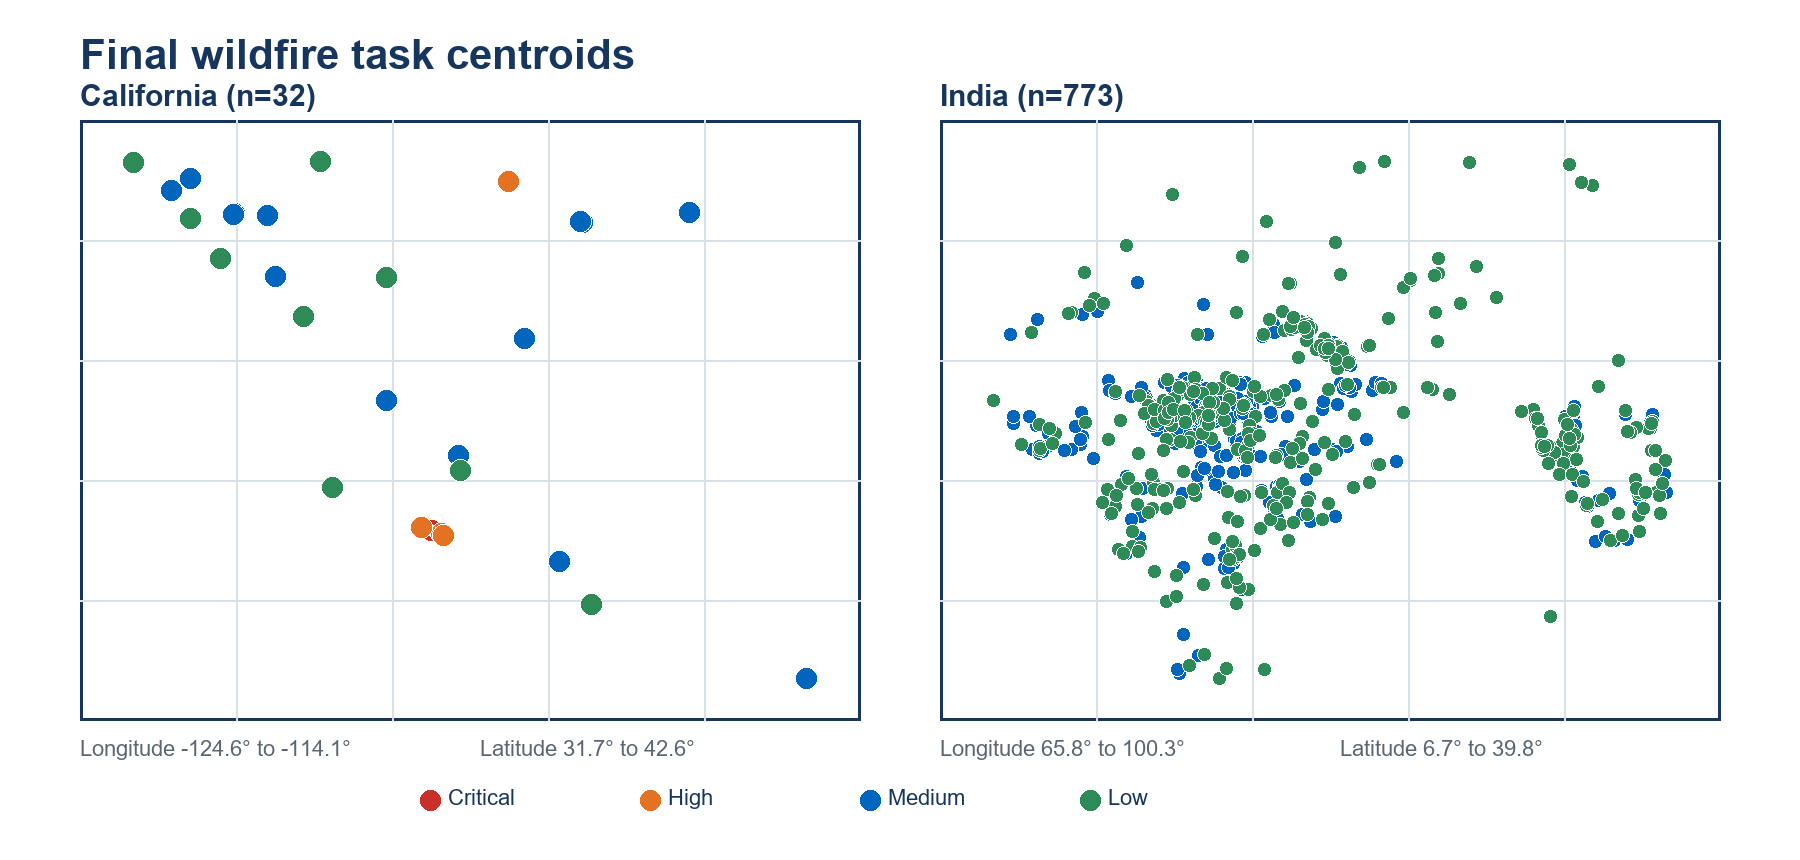
\includegraphics[width=0.94\textwidth]{wildfire_task_map.png}
\caption{Final de-duplicated Sentinel-3 wildfire-task centroids for California and India, coloured by priority class. The figure is generated directly from the 805-row task input.}
\label{fig:wildfire_task_map}
\end{figure}

\section{Processing Pipeline}

Figure~\ref{fig:task_pipeline} summarizes the task-generation workflow. Product discovery and NetCDF extraction are followed by filtering, clustering, scoring, de-duplication, and export. Every transformation has a narrower purpose than the previous one: filtering rejects weak or irrelevant detections, clustering forms candidate fire regions, scoring ranks those regions, and de-duplication determines which candidates become independent DSS tasks.

\begin{figure}[htbp]
\centering
\begin{tikzpicture}[every node/.style={font=\small}, box/.style={draw=TUMBlue,rounded corners,fill=TUMBlue!5,minimum height=1.05cm,text width=2.35cm,align=center}, arr/.style={->,thick,TUMBlue}]
\node[box] (search) at (0,1.5) {Product search and download};
\node[box] (extract) at (3.2,1.5) {SLSTR FRP NetCDF extraction};
\node[box] (filter) at (6.4,1.5) {Region, date, quality, FRP filtering};
\node[box] (cluster) at (6.4,0) {DBSCAN fire-region clustering};
\node[box] (score) at (3.2,0) {Priority score and deadline};
\node[box] (dedup) at (0,0) {Product, hotspot, and task de-duplication};
\node[box] (export) at (3.2,-1.5) {DSS-ready task CSV};
\draw[arr] (search)--(extract); \draw[arr] (extract)--(filter); \draw[arr] (filter)--(cluster);
\draw[arr] (cluster)--(score); \draw[arr] (score)--(dedup); \draw[arr] (dedup.south) |- (export.west);
\end{tikzpicture}
\caption{Sentinel-3 wildfire-task generation and export workflow.}
\label{fig:task_pipeline}
\end{figure}

\subsection{Product and NetCDF selection}

A downloaded \texttt{.SEN3} directory corresponds to one SLSTR Level-2 FRP product granule. The product name contains the sensing interval, while a later timestamp records product generation. The region of interest is applied after reading the geolocated fire pixels because the product is not intrinsically limited to California or India.

The first pipeline version successfully automated search, download, extraction, and scoring but read repeated product content. The second version corrected invalid confidence values and exact duplicates. The third version, used for the final task input, introduced four de-duplication levels:

\begin{enumerate}
\item \textbf{product level:} each \texttt{.SEN3} product is read once;
\item \textbf{NetCDF level:} the primary FRP file is selected instead of indiscriminately reading support files;
\item \textbf{hotspot level:} exact and near-duplicate detections are removed using rounded position, time, and FRP; and
\item \textbf{task level:} nearby candidates representing the same fire region on the same day are merged, retaining the highest-priority representative.
\end{enumerate}

The fall in regional total FRP between versions is therefore an expected consequence of removing repeated observations, not a loss of physical signal. Table~\ref{tab:sentinel_versions} records this development history. The values are included to document why the third version is used and are not architecture results.

\begin{table}[htbp]
\centering
\caption{Sentinel-3 pipeline refinement and regional total FRP reported during development.}
\label{tab:sentinel_versions}
\begin{tabularx}{\textwidth}{C{0.08\textwidth}Y r r}
\toprule
Version & Main change & California FRP (MW) & India FRP (MW) \\
\midrule
v1 & Initial automated search, extraction, and scoring; repeated reading remained & 137,753 & 323,677 \\
v2 & Revised confidence handling and exact hotspot de-duplication & 68,876 & 161,811 \\
v3 & Product-, NetCDF-, hotspot-, and task-level de-duplication & 22,686 & 34,595 \\
\bottomrule
\end{tabularx}
\end{table}

\subsection{FRP threshold and clustering}

Fire radiative power is used as an intensity variable because it is related to active biomass combustion and is more informative than an unweighted detection count \citep{Wooster2012}. Development experiments applied an FRP threshold of \SI{10}{\mega\watt} before clustering. This threshold removes weak thermal detections from task generation while retaining operationally meaningful active-fire signals.

DBSCAN groups detections using spatial density rather than a pre-declared number of clusters. Radius and minimum-sample sweeps were used during development to avoid the two extremes of treating every pixel as a separate task or merging geographically distant fires. A 10 km radius and \texttt{min\_samples}=3 were used in the documented FIRMS screening work; the Sentinel-3 task output retains the cluster centroid, approximate radius, number of detections, and product provenance. Isolated detections are preserved or rejected according to the pipeline rules rather than silently folded into the nearest cluster.

\section{Confidence Harmonization}

FIRMS and Sentinel-3 expose confidence differently. Sentinel-3 provides a numerical MWIR confidence percentage, which is divided by 100. FIRMS VIIRS provides categorical values that were mapped to 0.33, 0.66, and 1.00 for low, nominal, and high confidence. The harmonized value is a relative ranking variable, not a calibrated probability that a detection is a wildfire.

For Sentinel-3, invalid values such as $-1$ are not interpreted as zero confidence. They receive a neutral score of 0.50 and are flagged as missing. This prevents an unavailable field from suppressing a task while retaining transparency for later filtering. The task table also records the missing-confidence fraction and the minimum, maximum, and dominant confidence information of the contributing detections.

\section{Priority Score}

The task-priority score combines fire intensity, confidence, and cluster size. The FRP component first combines normalized total and maximum FRP:

\begin{equation}
S_{\mathrm{FRP}} = 0.60\,\mathcal{N}\!\left(\log(1+\mathrm{FRP}_{\mathrm{total}})\right)
+0.40\,\mathcal{N}\!\left(\log(1+\mathrm{FRP}_{\mathrm{max}})\right),
\label{eq:frp_score}
\end{equation}

where $\mathcal{N}(\cdot)$ denotes the declared normalization within the scoring dataset. The logarithm prevents a small number of extreme fires from determining the entire range. The final score is

\begin{equation}
S_{\mathrm{task}} = 0.50S_{\mathrm{FRP}}+0.30S_{\mathrm{conf}}+0.20S_{\mathrm{cluster}}.
\label{eq:task_score}
\end{equation}

Equation~\ref{eq:task_score} gives FRP the largest weight because it represents energetic strength. Confidence acts as a reliability modifier, and cluster size represents local spatial extent or density. The weights are an engineering model, not a learned clinical or civil-protection severity scale. This limitation is important because agricultural burning and industrial heat sources may still receive a high score if their physical inputs are large.

\section{Final Task Population}

Table~\ref{tab:task_population} describes the final task population. The India event contributes 96.0\% of the tasks, but California contains a greater fraction of urgent tasks. This is why regional totals are normalized per task before communication burden is compared.

\begin{table}[htbp]
\centering
\caption{Final de-duplicated Sentinel-3 task population used by the nominal campaign.}
\label{tab:task_population}
\begin{tabular}{lrrrrr}
\toprule
Region & Critical & High & Medium & Low & Total \\
\midrule
California & 1 & 6 & 16 & 9 & 32 \\
India & 0 & 11 & 395 & 367 & 773 \\
\midrule
Total & 1 & 17 & 411 & 376 & 805 \\
\bottomrule
\end{tabular}
\end{table}

Figure~\ref{fig:priority_distribution} presents both absolute counts and within-region shares. The left panel makes the communication-load difference explicit, while the right panel shows that California has a markedly larger urgent-task share. Reporting both views avoids letting the India count dominate the visual interpretation.

\begin{figure}[htbp]
\centering
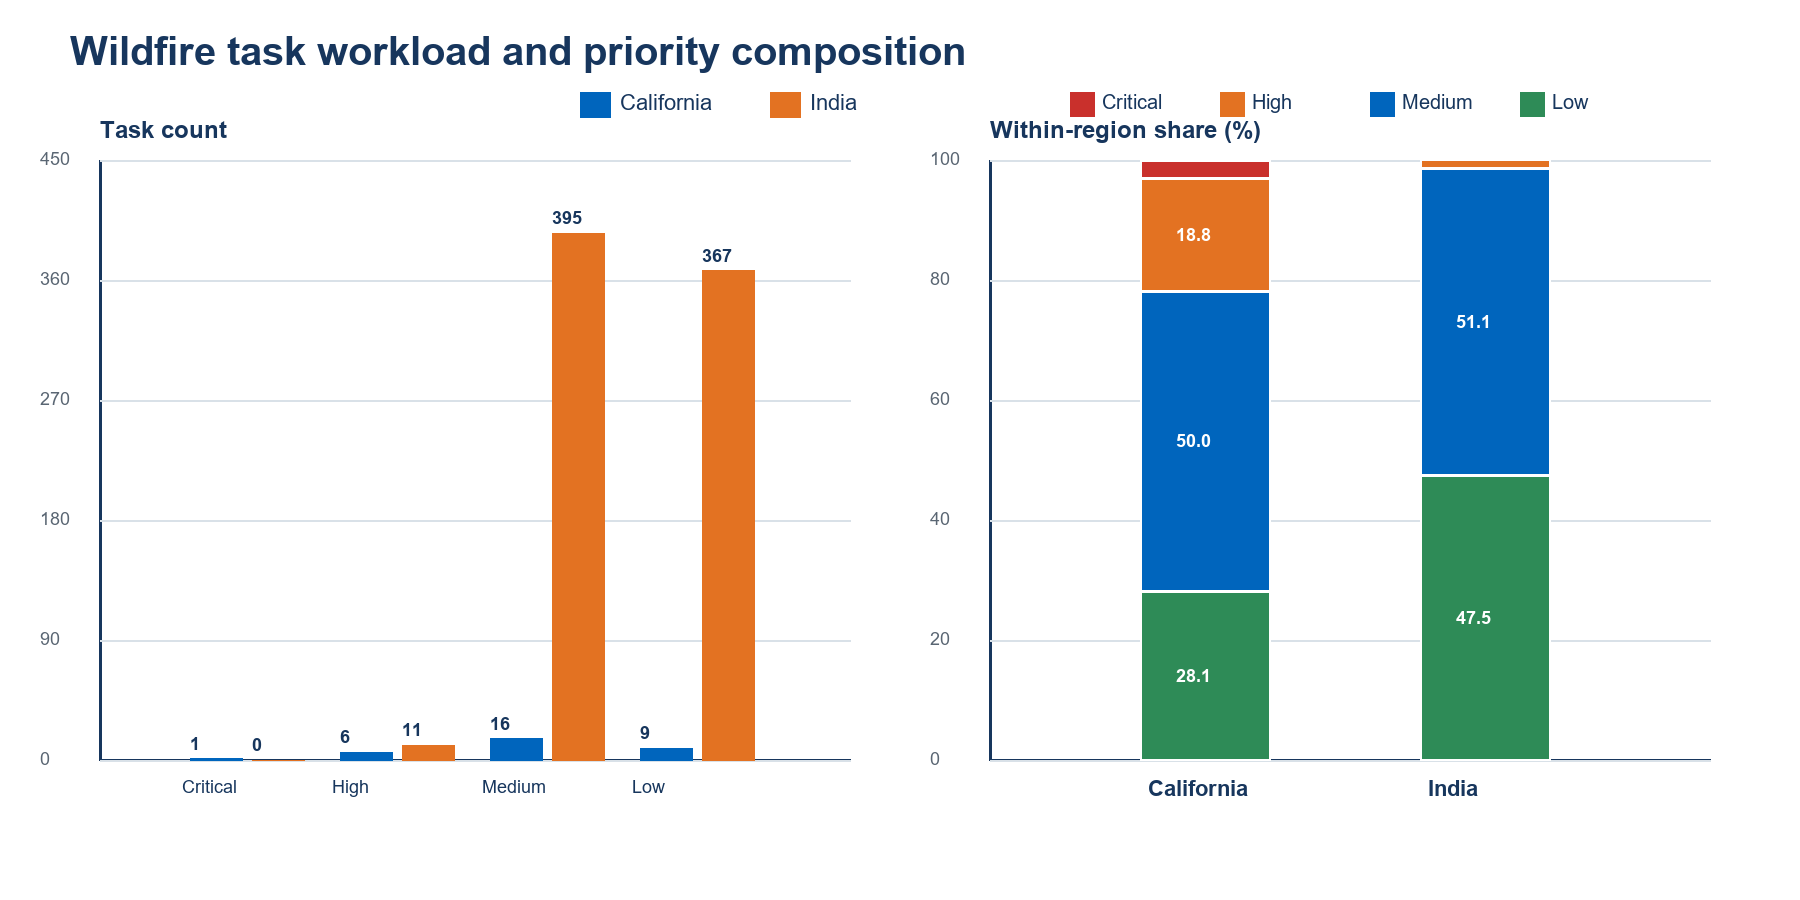
\includegraphics[width=0.94\textwidth]{priority_distribution.png}
\caption{Absolute regional workload and priority composition of the final task set.}
\label{fig:priority_distribution}
\end{figure}

Priority determines both the response deadline and nominal packet size as shown in Table~\ref{tab:priority_model}. These packet sizes represent the task-allocation message carried by the simulated network, not raw imagery. Therefore, the nominal communication results concern dissemination of observation requests rather than transfer of full SLSTR products.

\begin{table}[htbp]
\centering
\caption{Priority-dependent response deadlines and task packet sizes in the final nominal campaign.}
\label{tab:priority_model}
\begin{tabular}{lrrl}
\toprule
Priority & Deadline (min) & Packet size (Mbit) & Operational interpretation \\
\midrule
Critical & 30 & 2.0 & Immediate high-severity follow-up request \\
High & 60 & 1.5 & Urgent follow-up request \\
Medium & 180 & 1.0 & Time-sensitive routine request \\
Low & 360 & 0.5 & Lower-urgency monitoring request \\
\bottomrule
\end{tabular}
\end{table}

Because priority changes simultaneously with size and deadline, the nominal campaign is not a controlled task-size experiment. A comparison between Critical and Low packets would mix data volume, urgency, geography, and fire severity. Chapter~7 therefore defines a separate task-size sweep that holds task identity and deadline constant while applying controlled multipliers.

\section{DSS Task Schema}

The source and simulator fields are summarized in Table~\ref{tab:task_schema}. Every field shown is either present in the de-duplicated CSV or created deterministically by the task loader. The complete schema is retained in the appendix and software release.

\begin{table}[htbp]
\centering
\caption{Core task fields transferred from the Sentinel-3 pipeline to the DSS simulator.}
\label{tab:task_schema}
\begin{tabularx}{\textwidth}{L{0.27\textwidth}L{0.15\textwidth}Y}
\toprule
Field & Unit/type & Meaning \\
\midrule
\path{task_id} & string & Stable task identifier within the source table \\
\path{region}, \path{date} & category/date & Event-region membership and source day \\
\path{timestamp_utc} & UTC time & Task release time before deadline construction \\
\path{centroid_lat/lon} & degrees & Representative fire-region position \\
\path{num_detections} & count & Detections supporting the clustered task \\
\path{approx_radius_km} & km & Approximate spatial radius of the task cluster \\
\path{mean/max/total_frp_mw} & MW & Fire-radiative-power summaries \\
\path{confidence_score} & 0--1 & Harmonized relative confidence score \\
\path{task_priority_score} & 0--1 & Composite score from Equation~\ref{eq:task_score} \\
\path{priority_class} & category & Critical, High, Medium, or Low \\
\path{required_response_time_min} & min & Deadline offset from task release \\
\path{task_size_mbits} & Mbit & Simulator-assigned packet size \\
\bottomrule
\end{tabularx}
\end{table}

\section{Validation and Limitations of the Task Dataset}

The strongest event-level validation is the Madre Fire. Both Sentinel-3 and FIRMS produced high-priority tasks near the reported event location during the California window. The India task set has broader regional support but weaker named-incident traceability. The data are consequently appropriate for architecture stress testing and selected event validation, but they are not a labelled benchmark for wildfire classification accuracy.

Several limitations remain. Bounding-box filtering can retain points outside the political region unless a polygon mask is applied. Cloud, smoke, and overpass time change the detections available to each sensor. FIRMS and Sentinel-3 cannot be compared by regional FRP alone because their sensing, sampling, and de-duplication differ. A more defensible agreement study would match tasks in space and time and report centroid distance, priority-class agreement, FRP ratio, and unmatched counts.

For this thesis, the final task table is frozen before architecture evaluation. All 891 cases within a region use the same task source and row count, which prevents architecture comparisons from being contaminated by changing wildfire inputs. The remaining uncertainty belongs to external validity: the preferred architecture could differ for another season, sensor, region, or priority model.

\chapter{System Model and Methodology}
\section{Methodological Overview}

The final workflow converts frozen wildfire detections into time-dependent tasks, evaluates a factorial Walker-constellation design space, and replays each architecture under nominal, policy, load, and failure scenarios. The workflow deliberately separates four layers: task data, physical opportunities, allocation logic, and evaluation. This separation makes it possible to change a routing policy or inject a failure without silently changing the task set or orbital geometry.

Figure~\ref{fig:method_workflow} shows the dependency chain. A task cannot be sent before release, a transfer cannot exceed a contact-window capacity, and an observation is successful only if an observing satellite already holds the task and acts before the deadline.

\begin{figure}[htbp]
\centering
\begin{tikzpicture}[every node/.style={font=\small}, box/.style={draw=TUMBlue,rounded corners,fill=TUMBlue!5,minimum height=0.95cm,text width=2.35cm,align=center}, arr/.style={->,thick,TUMBlue}]
\node[box] (tasks) at (0,2.8) {Freeze regional wildfire tasks};
\node[box] (arch) at (3.2,2.8) {Generate Walker architecture};
\node[box] (states) at (6.4,2.8) {Propagate states and label CNs};
\node[box] (windows) at (6.4,1.4) {Build link and observation windows};
\node[box] (scenario) at (3.2,1.4) {Apply scenario transformations};
\node[box] (route) at (0,1.4) {Replay temporal routing};
\node[box] (eval) at (0,0) {Evaluate reception and observation};
\node[box] (export) at (3.2,0) {Checkpoint typed Parquet tables};
\node[box] (post) at (6.4,0) {Validate, aggregate, and rank};
\draw[arr] (tasks)--(arch); \draw[arr] (arch)--(states); \draw[arr] (states)--(windows);
\draw[arr] (windows)--(scenario); \draw[arr] (scenario)--(route); \draw[arr] (route)--(eval);
\draw[arr] (eval)--(export); \draw[arr] (export)--(post);
\end{tikzpicture}
\caption{Fresh Full891 V2 simulation and post-processing workflow.}
\label{fig:method_workflow}
\end{figure}

\section{Task Input and Temporal Horizon}

The campaign consumes a deterministic CSV rather than querying a live service during simulation. The file contains 805 frozen tasks: 32 for California and 773 for India. Each row supplies a stable identifier, region, position, release epoch, priority, deadline, task-message size, and source provenance. Chapter~3 describes the upstream Sentinel-3 processing and the supporting FIRMS screening.

The original UTC epochs are retained. For each region, the simulation duration is

\begin{equation}
T_{\mathrm{sim}}=\max\left(72\ \mathrm{h},\;d_{\max}-r_{\min}+6\ \mathrm{h}\right),
\end{equation}

where $r_{\min}$ is the first release and $d_{\max}$ is the latest deadline. This gives approximately 73.134 hours for California and 73.659 hours for India in Fresh V2. Priority-dependent deadlines are 30, 60, 180, and 360 minutes for Critical, High, Medium, and Low tasks. The associated nominal messages are 2.0, 1.5, 1.0, and 0.5 Mbit. These are simulated task descriptions, not downloaded sensor-image volumes.

\section{Walker Constellation and Central-Node Assignment}

An architecture is represented by total satellite count $T$, plane count $P$, altitude $H$, inclination $I$, central-node fraction $C$, and phasing $F=1$. The complete grid is

\begin{equation}
\{60,120,180\}\!\times\!\{3,5,10\}\!\times\!\{500,800,1000\}
\!\times\!\{60,80,98.6\}\!\times\!\{0,10,\ldots,100\},
\end{equation}

which gives $3^4\times11=891$ cases per region. For example,

\begin{equation}
\texttt{T060\_P10\_H0800\_I0986\_CN040\_F1}
\end{equation}

denotes 60 spacecraft in 10 planes at \SI{800}{\kilo\metre}, \SI{98.6}{\degree} inclination, with 40 percent (24) assigned the central-node role.

The nodes share the same orbital and sensing model; ``central'' denotes a communication and routing role, not a separate relay shell or a fully costed hardware class. Central nodes are spread across planes as evenly as integer constraints permit and then spaced within each plane. This deterministic placement prevents arbitrary clustering from confounding a fraction sweep. It is a reproducible baseline rather than a placement optimum.

\section{Orbit and Observation Opportunity Model}

The orbital layer uses circular two-body propagation on a spherical rotating Earth, consistent with the integrated TAT-C-based workflow \citep{TATC}. Fresh V2 uses $R_E=\SI{6378.137}{\kilo\metre}$, $\mu=\SI{398600.4418}{\kilo\metre\cubed\per\second\squared}$, Earth rotation $7.2921159\times10^{-5}$ rad/s, and a \SI{60}{\second} time step. Walker plane population and phasing are validated for every generated case.

An observation opportunity exists when the satellite--task ground distance is within the fixed \SI{700}{\kilo\metre} access radius. Let $O_{is}$ be candidate times for task $i$ and satellite $s$, $r_i$ the release time, $d_i$ the deadline, and $a_{is}$ the time at which $s$ receives the task. A valid follow-up time is

\begin{equation}
t^{\mathrm{obs}}_i=\min_s\{t\in O_{is}:t\geq\max(r_i,a_{is})\ \land\ t\leq d_i\}.
\label{eq:valid_observation}
\end{equation}

The access radius is a mission-level approximation. It does not model cloud, smoke, lighting, field of view, slew, image quality, energy, storage, or conflicts between simultaneous observations. No Fresh V2 observation-radius sweep is presently available.

\section{Communication Opportunities and Link Capacity}

All unordered satellite pairs are first tested for physical contact; scenario topology rules are applied later. The ground segment contains the Munich station with a \SI{10}{\degree} minimum elevation. Each communication window stores endpoints, type, start and end time, effective data rate, usable duration, and capacity.

Satellite-to-satellite capacity is calculated by the active V19 UHF link-budget implementation, using a \SI{2}{\watt}, \SI{437}{\mega\hertz}, \SI{9.6}{\kilo\hertz} channel and 9.6~ksymbol/s signal together with the configured gains, losses, sensitivity, and a 1.5 central-node link-budget boost. The resulting effective rate is capped near \SI{19.2}{\kilo\bit\per\second}. A legacy configuration field named \path{sat_sat_data_rate_bps} contains 250,000 bit/s but is not consumed by the active calculation and is therefore not used as a scientific claim. Satellite-to-ground windows use \SI{100}{\kilo\bit\per\second}.

For window $w$ of usable duration $\Delta t_w$, utilization factor $\eta_w$, and effective rate $R_w$, the capacity is

\begin{equation}
B_w=\frac{R_w\Delta t_w\eta_w}{10^6}\quad[\mathrm{Mbit}].
\label{eq:window_capacity}
\end{equation}

Fresh V2 sets $\eta_w=1$. A window records potential capacity; a transfer event records actual use. These quantities are never treated as interchangeable.

\section{Topology and Temporal Routing}

Three topology-policy variants are replayed:

\begin{description}[leftmargin=3.0cm,style=nextline]
\item[Central-only] An inter-satellite link is usable only when at least one endpoint is central. CN0 therefore has no inter-satellite link and relies on ground uplink; it is not a peer-to-peer baseline.
\item[Peer-only] All feasible inter-satellite links are usable and routing does not privilege the central label.
\item[Hybrid] All feasible links are usable and the selection order prefers central-node forwarding.
\end{description}

Ground initially knows each task at release. The evaluator traverses communication windows in time order and transmits whole messages only: fragmentation is not implemented. A node can forward a task only after full reception; duplicate reception does not increase coverage. Candidate messages are ordered by priority, deadline, central-node preference, and target utility, then admitted only when residual window capacity and policy limits allow.

The nominal-original scenario uses the central-only/targeted policy, useful-recipient and deadline targeting, at most three forwarding hops, three observer copies, and five central-node copies. The \emph{unlimited useful-deadline} diagnostic retains the useful-recipient and deadline definition but removes these hop and copy limits. It reveals latent architecture capability and must not be confused with the implementable nominal policy.

Accepted transfers retain task, sender, receiver, time, link type, message size, and hop depth. The algorithm is greedy and causal; it is not a globally optimized temporal multicommodity-flow solution.

\section{Scenario Transformations}

Fresh V2 evaluates 539 declared scenarios per case. Deterministic policy and task-size scenarios are complemented by repeated stochastic failures. A replicate is an independent rerun of the same architecture and severity with a different deterministic random seed; it measures variability due to which satellite, central node, link window, or outage interval is selected.

Random satellite and random central-node failures remove selected nodes, their incident links, and their observation opportunities. Targeted central-node failure removes nodes ranked by incident capacity and degree. Link-window outage removes selected window rows. Ground-station outage disables a sampled interval. Capacity degradation scales communication capacity. Combined stress varies task size and satellite failure together. Every transformed scenario reruns routing and observation evaluation; graph statistics alone are not accepted as robustness evidence.

The random seed is derived from the campaign seed, case identifier, scenario identifier, and replicate number using SHA-256. The first eight digest bytes define the numeric seed. Consequently, scenario outcomes are invariant to worker count and completion order.

\section{Outcome and Resource Metrics}

Observation fulfilment for $N$ tasks is

\begin{equation}
F_{\mathrm{obs}}=\frac{100}{N}\sum_{i=1}^{N}\mathbb{I}[t_i^{\mathrm{obs}}\le d_i].
\end{equation}

Let $E_i$ be the useful-recipient set after the active failure transformation and $R_i(d_i)$ the unique useful recipients reached by deadline. Mean useful coverage uses

\begin{equation}
Q_i=100\frac{|R_i(d_i)|}{|E_i|},
\end{equation}

and strict dissemination is

\begin{equation}
S^{\mathrm{useful}}_{100,i}=\mathbb{I}[E_i\neq\emptyset\ \land\ R_i(d_i)=E_i].
\end{equation}

The campaign stores original and surviving denominators separately so that failed nodes cannot create an artificial improvement. If complete dissemination occurs, $T_{100,i}$ is the release-to-last-useful-reception time. The reported P100 $T_{100}$ is the worst completed task in the case; it is censored when any required completion is unavailable. It is not first-reception latency. The Fresh V2 canonical case table does not expose a separate first-reception field, so this report does not relabel $T_{100}$ as first reception.

Communication burden is reported with transferred Mbit, transfer-event count, used-capacity percentage, central-node traffic share, peak node load, and a Gini coefficient over node-sent data. Performance and burden are reported as separate raw metrics before any composite score is introduced.

\section{Checkpointing, Parquet Output, and Deterministic Resume}

Each base architecture is one worker job that evaluates its eleven central-node cases. Scenario rows are written in batches of 20 to temporary files and atomically renamed when complete. On restart, the runner reads completed scenario identifiers and evaluates only the missing set. A \path{_SUCCESS.json} marker is created only after all expected scenario identifiers are present; exceptions create a \path{_FAILED.json} marker.

The tables are stored in Apache Parquet: a typed, columnar format with Zstandard compression. Parquet is intended for reliable analytical reading by Python, R, DuckDB, Spark, or similar tools rather than manual editing in a text editor. It preserves numeric types, compresses repeated columns efficiently, and allows column-selective reads. The principal case products are scenario metrics, task metrics, transfer events, central-node distribution, constellation nodes, manifests, and validation records.

Worker count is limited by the minimum of the configured maximum, operating-system CPU availability, and an available-memory estimate of approximately \SI{3}{\gibi\byte} per worker. Changing 8 workers to 16 or 25 alters wall-clock time and the recorded execution fingerprint, but not the scientific seed or case definition. Scientific changes require a new output root; worker-only changes may safely resume the same root.

\section{Validation before Inference}

Post-processing follows a fixed gate sequence: read-only inventory, schema and traceability, completeness, independent metric recomputation, effect summaries, exact Pareto analysis, objective-weight sensitivity, robustness, and limitations. Duplicate scenario keys produced by interrupted resume are resolved deterministically before aggregation. Failed and censored observations remain visible rather than being silently dropped.

No ranking is performed until the relevant validation gates pass. The California Fresh V2 archive contains one incomplete case, which is excluded from comparisons that require all 539 scenarios. The integrity evidence is reported in Chapter~7 and Appendix~C.

\section{Pareto and Objective-Weight Method}

The preferred architecture is treated as a decision conditional on mission priorities. First, exact dominance is evaluated on raw benefits and burdens. A case is Pareto efficient if no other case is at least as good on every objective and strictly better on one.

For the weight-consistent analysis, the performance pillar is

\begin{equation}
P=0.25\widetilde F_{\mathrm{obs}}+0.25\widetilde S_{100}
+0.25\widetilde Q+0.25\widetilde T,
\end{equation}

where $\widetilde T$ is inverse min--max P100 $T_{100}$ and censored cases receive zero timeliness benefit rather than being removed. The resource-efficiency pillar is

\begin{equation}
R=0.40(1-\widetilde N_{\mathrm{sat}})+0.20(1-\widetilde N_{\mathrm{CN}})
+0.20(1-\widetilde B)+0.20(1-\widetilde E),
\end{equation}

where $B$ is transferred data and $E$ transfer-event count. The 40/20/20/20 split is a declared engineering preference: fleet size receives twice the weight of each remaining burden. It is not inferred from prices or claimed as universally correct.

The high-level utility is

\begin{equation}
U(\lambda)=\lambda P+(1-\lambda)R,\qquad 0\le\lambda\le1.
\end{equation}

Sensitivity uses 10,000 reproducible draws with seed 20260825: $\lambda\sim\mathrm{Uniform}(0,1)$, performance weights from Dirichlet$(1,1,1,1)$, and resource weights from Dirichlet$(4,2,2,2)$. Winner frequency is a stability diagnostic over a declared preference distribution, not a probability that an architecture is objectively correct.

\section{Implementation Ownership and Method Boundaries}

Vincenzo Messina supplied the communication-model and TAT-C basis. The author implemented the wildfire-task processing, simulator integration, central-node placement, scenario runner, checkpoint/resume controls, validation, post-processing, statistical analysis, figures, and report.

The method evaluates task-message dissemination and follow-up opportunity under simplified orbit, sensing, and communications assumptions. It does not model image downlink, emergency alert delivery, operational response, monetary lifecycle cost, or a hardware-differentiated central-node subsystem. Conclusions therefore apply to the implemented communication/routing role and the tested task sets.

\chapter{Experimental Design and Reproducibility}
\section{Two Evidence Layers}

The thesis contains two validated but non-interchangeable result layers. Table~\ref{tab:evidence_layers} defines their role. The earlier nominal campaign is the only completed two-region evidence and supports the California--India contrast in Chapter~6. Fresh Full891 V2 adds scenario replay, robustness, task-size, policy, and objective-weight analysis, but only the California output is currently available. Numerical values are never averaged across these versions.

\begin{table}[htbp]
\centering
\caption{Result layers and permitted use.}
\label{tab:evidence_layers}
\begin{tabularx}{\textwidth}{L{0.22\textwidth}L{0.25\textwidth}Y}
\toprule
Layer & Coverage & Role in this report \\
\midrule
Earlier nominal & 891 California + 891 India architecture cases & Validated regional baseline and paired architecture comparison \\
Fresh Full891 V2 & 891 California case identifiers; 890 complete & Main scenario, robustness, task-size, policy, and decision evidence \\
Fresh Full891 V2 India & Run/validation pending & Required before Fresh V2 regional conclusions can be finalized \\
\bottomrule
\end{tabularx}
\end{table}

\section{Common Architecture Grid}

Both layers use the factorial grid in Table~\ref{tab:factor_grid}. Eleven central-node levels share each of 81 base architectures, allowing a within-geometry fraction sweep. The design contains 891 architecture identifiers per region.

\begin{table}[htbp]
\centering
\caption{Architecture factors in the Full891 design.}
\label{tab:factor_grid}
\begin{tabularx}{\textwidth}{L{0.27\textwidth}L{0.28\textwidth}Y}
\toprule
Factor & Levels & Experimental role \\
\midrule
Total satellites & 60, 120, 180 & Fleet scale and resource proxy \\
Orbital planes & 3, 5, 10 & Spatial distribution and contact geometry \\
Altitude & 500, 800, 1000 km & Access/contact geometry \\
Inclination & 60, 80, 98.6 deg & Regional access geometry \\
Central-node fraction & 0, 10, $\ldots$, 100\% & Degree of centralization \\
Walker phasing & $F=1$ & Fixed control \\
\bottomrule
\end{tabularx}
\end{table}

\section{Earlier Two-Region Nominal Campaign}

The earlier campaign contains one deterministic nominal evaluation for every architecture in California and India, for 1,782 analytical case rows. All expected cases passed completeness and configuration checks. Ten case metrics were independently recomputed, giving 17,820 comparisons and no failure at tolerance $10^{-6}$. This layer predates the Fresh V2 scenario contract and is retained because it supplies the completed regional comparison requested in the research questions.

Its interpretation is deliberately limited. It supports statements about the observed two-event baseline under its frozen configuration, not Fresh V2 failure retention or task-size sensitivity. Chapter~6 labels every table and figure from this layer.

\section{Fresh Full891 V2 Scenario Matrix}

Fresh V2 creates 539 scenario definitions for each architecture. Table~\ref{tab:v2_scenario_matrix} shows the construction. Stochastic families use 30 replicates per severity. Deterministic families are evaluated once per level.

\begin{table}[htbp]
\centering
\small
\caption{Fresh V2 scenario contract for each architecture case.}
\label{tab:v2_scenario_matrix}
\begin{tabularx}{\textwidth}{L{0.30\textwidth}L{0.45\textwidth}r}
\toprule
Scenario family & Construction & Rows \\
\midrule
Core, policy, and unlimited & Seven named scenarios & 7 \\
Task size & $0.5\times$, $1\times$, $2\times$, $4\times$ & 4 \\
Random satellite failure & Four levels $\times$ 30 replicates & 120 \\
Random central-node failure & Four levels $\times$ 30 replicates & 120 \\
Link-window outage & Four levels $\times$ 30 replicates & 120 \\
Ground-station outage & Four levels $\times$ 30 replicates & 120 \\
Targeted central-node failure & Four deterministic levels & 4 \\
Capacity degradation & Four deterministic levels & 4 \\
Combined stress & Two sizes $\times$ two satellite-failure levels $\times$ 10 replicates & 40 \\
\midrule
Total & & 539 \\
\bottomrule
\end{tabularx}
\end{table}

Here a replicate means a repeated random trial at the same architecture, scenario family, and severity. The architecture and tasks remain fixed, but the failed nodes, removed links, or outage interval can differ. Thirty replicates estimate the distribution of a random-failure response; they are not 30 different architectures.

If both regions complete the contract, the design contains $1{,}782\times539=960{,}498$ expected scenario rows. CN0 has no central nodes, so 124 central-node-failure rows per CN0 case are explicitly \texttt{NOT\_APPLICABLE}; the two-region expected total is 20,088. These rows remain in the manifest and are not treated as failures or silently dropped.

\section{California Fresh V2 Integrity Audit}

The California archive was inspected before numerical aggregation. Table~\ref{tab:ca_integrity} records the result. The expected full total is $891\times539=480{,}249$ rows. Interrupted/resumed batches produced 4,269 duplicate scenario keys; deterministic de-duplication retains the final unique record for each declared key.

\begin{table}[htbp]
\centering
\caption{California Fresh V2 campaign integrity.}
\label{tab:ca_integrity}
\begin{tabular}{lr}
\toprule
Quantity & Value \\
\midrule
Base-architecture directories & 81 \\
Architecture case directories & 891 \\
Complete success markers & 890 \\
Failure markers & 0 \\
Expected scenarios per complete case & 539 \\
Raw scenario rows & 484,379 \\
Unique rows across all cases & 480,110 \\
Resume duplicates removed & 4,269 \\
Unique rows in success cases & 479,710 \\
Completed / not-applicable / failed status rows & 469,666 / 10,044 / 0 \\
Architecture-validation checks passed & 19,179 of 19,179 \\
\bottomrule
\end{tabular}
\end{table}

The incomplete identifier is
\begin{center}
\texttt{T180\_P10\_H1000\_I0986\_CN100\_F1}.
\end{center}
It contains 400 of 539 rows and lacks 99 ground-station-outage and 40 combined-stress evaluations. It is retained in the inventory but excluded whenever a complete scenario comparison is required. This leaves 890 complete cases. Eighty of the 81 base geometries have a fully balanced 11-level CN sweep, giving 880 cases for balanced central-node marginal analysis.

Two configuration fingerprints occur: one for 889 cases and one for two cases. Field-level comparison attributes the difference to worker/runtime provenance, not tasks, scientific configuration, seeds, or scenario definitions. The worker change is therefore reported but does not invalidate the science.

\begin{figure}[htbp]
\centering
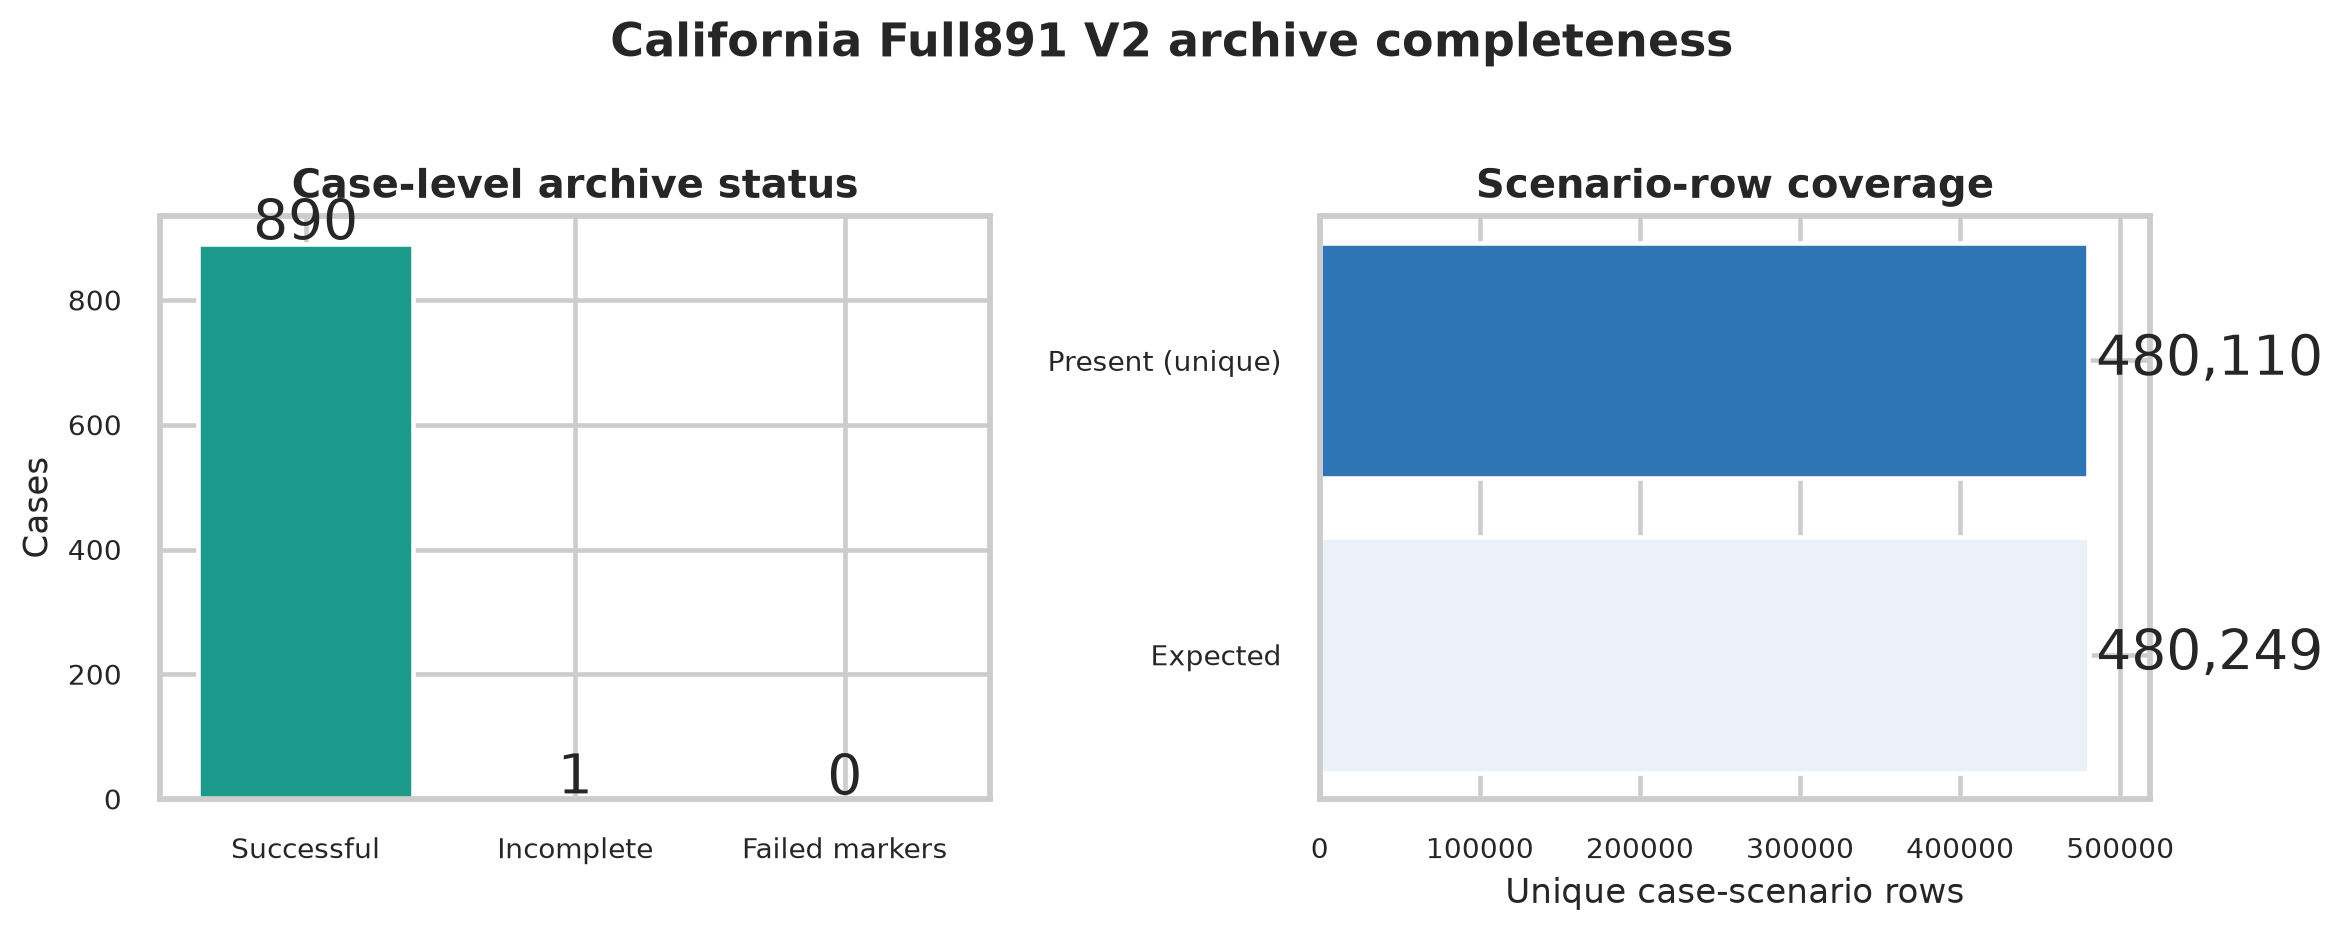
\includegraphics[width=0.82\textwidth]{01_archive_completeness.png}
\caption{California Fresh V2 completeness and scenario-family coverage after deterministic de-duplication.}
\label{fig:ca_completeness}
\end{figure}

\section{Validation Gates and Claim Freeze}

The checking method applies the following gates in order:

\begin{enumerate}
\item inventory paths, manifests, markers, and expected identifiers without altering raw output;
\item confirm schema, types, join keys, task provenance, and scenario traceability;
\item check completeness, uniqueness, status, and explicit not-applicable rows;
\item recompute metrics from lower-level task/transfer evidence where retained;
\item calculate paired effects and architecture sweeps only on eligible cases;
\item construct the exact Pareto set before applying weights;
\item run objective-weight and robustness sensitivity with declared seeds; and
\item write a claim ledger containing both supported conclusions and unavailable evidence.
\end{enumerate}

This order prevents a visually plausible ranking from masking missing cases, duplicate resume rows, a changed denominator, or censored latency. Raw observations remain visible beside normalized scores. A result is called robust only after the physical/temporal scenario has been replayed; a nominal task failure label is not a robustness experiment.

\section{Analysis Populations}

Different questions require different subsets:

\begin{itemize}
\item all 891 identifiers for archive inventory;
\item 890 complete cases for main California Fresh V2 summaries;
\item 880 cases in 80 complete base sweeps for balanced CN-fraction curves;
\item eligible cases within each scenario family after explicit \texttt{NOT\_APPLICABLE} handling;
\item 48 cases on the original six-objective unlimited Pareto set; and
\item 108 cases on the recomputed eight-objective frontier used for weight analysis.
\end{itemize}

The population is stated with each analysis. This is particularly important for conditional P100 $T_{100}$, which exists for 824 of the 890 unlimited cases, and for CN-failure scenarios, which do not apply to CN0.

\section{Output Contract and Post-Processing Inputs}

Each case folder contains a manifest, architecture validation, central-node distribution, constellation nodes, compressed scenario metrics, task metrics, and selected transfer events. Scenario and task tables are partitioned into files such as \path{case_metrics_part_0000.parquet}. A success marker closes the case only after the expected scenario identifiers are present.

The post-processing release included with this report contains compact CSV/JSON summaries and figures rather than the full raw Parquet archive. The compact files preserve values used in the thesis and can be inspected with ordinary spreadsheet or text tools. The raw archive remains external because it is too large for normal Git history. Its directory and marker structure is described in Appendix~E.

\section{Statistical and Decision Analysis}

Central-node curves aggregate within complete base sweeps. Non-CN factor summaries are descriptive marginal means, and effect sizes are unadjusted one-factor $\eta^2$ values; neither is interpreted as a causal coefficient in the presence of interactions. Spearman correlation describes monotonic association only.

Robustness is reported primarily as paired percentage-point change from the same architecture's unlimited baseline. Replicate distributions are summarized across the 30 seeded draws. Task-size sensitivity compares the four deterministic multipliers. Policy ablation compares central, peer, and hybrid implementations, with implementation-equivalent outputs called out rather than counted as independent evidence.

The decision sequence is: apply mission feasibility thresholds, compute exact Pareto efficiency, show the raw performance/resource vector, apply declared weights, and vary those weights. Pure resource weighting may select a zero-performance case; pure performance weighting may select an extreme high-resource case. These endpoints demonstrate why weighted utility cannot substitute for engineering constraints.

\section{Compute Configuration and Resume Semantics}

The VM runner limits concurrent workers using CPU availability and free memory. A planning allowance of approximately \SI{3}{\gibi\byte} per worker prevents a nominal core count from exhausting RAM. A 16-worker setting is therefore safe only when the VM retains sufficient memory for the operating system and worker peaks.

Stopping between completed checkpoints does not invalidate completed scenario rows. On restart, the program recognizes completed identifiers and continues the missing set. Abrupt interruption can leave temporary or duplicate batch records, which is why post-processing de-duplicates declared keys and requires the success marker. Editing worker count does not accelerate workers already running; the new value takes effect only for a restarted/resumed launcher.

\section{Evidence Still Missing}

The Fresh V2 India output was still running or unavailable at the report freeze. The fixed-radius California archive also contains no observation-radius sensitivity, and its canonical case table contains no separate first-reception-latency field. These absences are recorded as limits, not filled from the earlier nominal layer. Once India passes the same gates, the regional comparison should be repeated on paired architecture identifiers and normalized per task.

\chapter{Validated Two-Region Nominal Baseline}
\section{Evidence-Layer Boundary}

This chapter reports the earlier validated nominal campaign: 891 California and 891 India architecture cases. It is retained because it is the completed two-region evidence layer. Its values are not Fresh Full891 V2 values and are not numerically combined with Chapter~7. The purpose of this chapter is to establish the regional baseline and show which architecture rankings transfer between the two event sets under the earlier frozen model.

\section{Result Status}

All results in this chapter passed the validation gates defined in Chapter~5. They supersede the numerical conclusions of still earlier V10, V16, V19, 30-hour screening, and fixed-architecture slide-deck experiments. They do not supersede Fresh V2; instead, Chapter~7 reports that later California scenario layer separately.

The analytical population contains 891 cases for California and 891 for India. Every case has the expected task count, and every required case status is completed. Core summary metrics were recomputed from lower-level outputs in 17,820 comparisons with zero failures at a tolerance of $10^{-6}$. The numerical evidence is therefore internally consistent even though external model-validity limitations remain.

\section{Regional Campaign Summary}

Table~\ref{tab:regional_summary} summarizes the full architecture population. India has a higher mean observation fulfilment but a lower mean useful-receiver fraction. Transfer events per task are nearly identical, whereas transferred data per task is higher for California because its priority mix contains proportionally more large urgent packets.

\begin{table}[htbp]
\centering
\caption{Region-normalized summary across all 891 cases per event region.}
\label{tab:regional_summary}
\begin{tabular}{lrrrrr}
\toprule
Region & Obs. (\%) & \Suseful\ (\%) & Receivers (\%) & Mbit/task & Events/task \\
\midrule
California & 47.468 & 0.624 & 13.868 & 5.884 & 6.186 \\
India & 55.066 & 0.462 & 12.060 & 4.620 & 6.202 \\
\bottomrule
\end{tabular}
\end{table}

The very low mean \Suseful\ values require careful interpretation. They do not mean that almost no task is observed: mean observation fulfilment is roughly 47--55 percent. They mean that completing dissemination to every simulator-defined useful recipient before each deadline is rare under the targeted policy, three-hop limit, and copy limits. Observation requires only one suitably timed observer, while \Suseful\ requires all useful recipients.

\section{Central-Node Fraction Effects}

Figure~\ref{fig:cn_sweep} contains the four principal central-node marginal responses. Each point averages 81 base architectures. The top-left panel shows a large gain when moving from 0 to 10 percent central nodes, followed by a slower increase and a decrease at 100 percent. The bottom-right panel shows an almost monotonic and strongly nonlinear latency reduction. The dissemination and receiver panels reveal the opposing effect: broad reach is highest at modest central-node fractions and decreases at high fractions.

\begin{figure}[htbp]
\centering
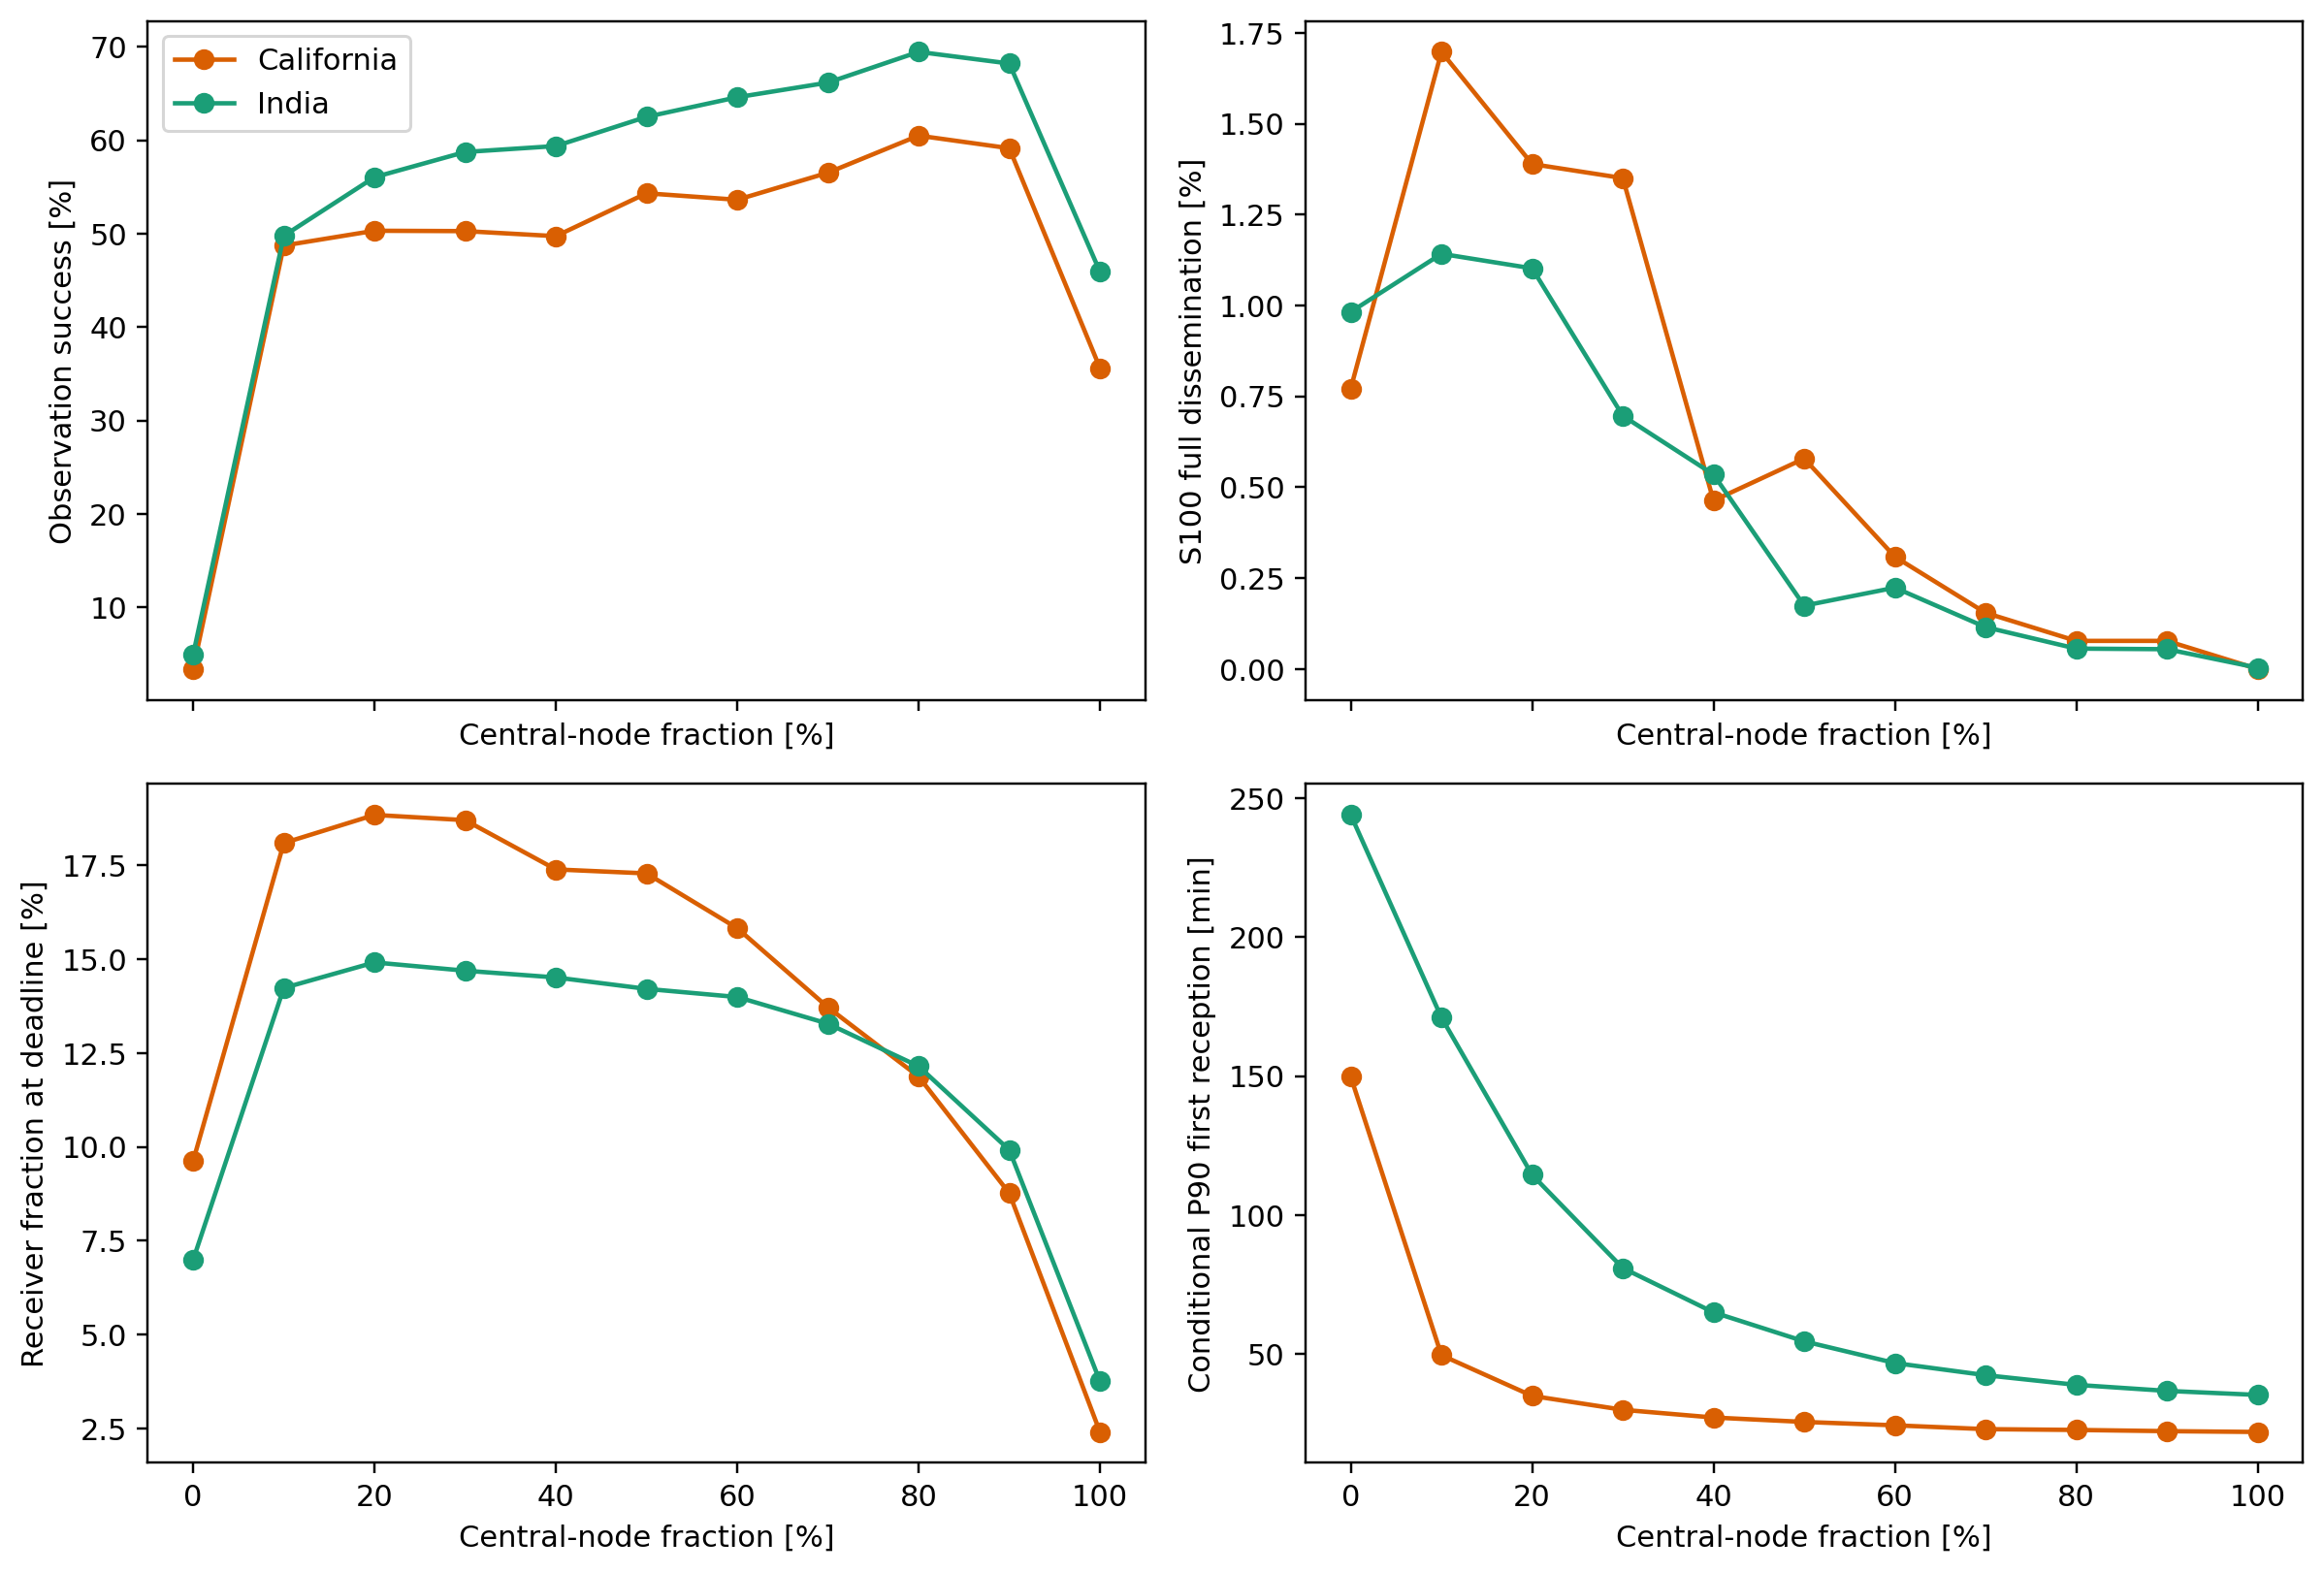
\includegraphics[width=0.98\textwidth]{01_cn_sweep_regional_summary.png}
\caption{Regional marginal response to central-node fraction across the full final grid. \Suseful\ denotes complete dissemination to all simulator-defined useful recipients.}
\label{fig:cn_sweep}
\end{figure}

Selected levels are reported in Table~\ref{tab:cn_selected}. The table illustrates the key engineering trade. For California, moving from CN0 to CN10 raises mean observation fulfilment from 3.40 to 48.73 percent and reduces P90 first-reception latency from 149.78 to 49.65 minutes. For India, the corresponding observation change is 4.92 to 49.77 percent and the latency change is 243.94 to 171.06 minutes. Further centralization continues to improve conditional first reception, but useful-recipient breadth does not continue to improve.

\begin{table}[htbp]
\centering
\caption{Selected regional central-node marginal means across 81 base architectures per row.}
\label{tab:cn_selected}
\begin{tabular}{lrrrrr}
\toprule
Region & CN (\%) & Obs. (\%) & \Suseful\ (\%) & Receivers (\%) & P90 first (min) \\
\midrule
California & 0 & 3.395 & 0.772 & 9.623 & 149.779 \\
California & 10 & 48.727 & 1.698 & 18.098 & 49.648 \\
California & 20 & 50.309 & 1.389 & 18.847 & 35.013 \\
California & 50 & 54.321 & 0.579 & 17.289 & 25.647 \\
California & 80 & 60.494 & 0.077 & 11.874 & 22.768 \\
California & 100 & 35.610 & 0.000 & 2.401 & 22.039 \\
\midrule
India & 0 & 4.921 & 0.982 & 6.988 & 243.944 \\
India & 10 & 49.766 & 1.142 & 14.235 & 171.061 \\
India & 20 & 56.044 & 1.102 & 14.916 & 114.486 \\
India & 50 & 62.503 & 0.174 & 14.211 & 54.628 \\
India & 80 & 69.460 & 0.056 & 12.148 & 38.982 \\
India & 100 & 45.925 & 0.003 & 3.752 & 35.365 \\
\bottomrule
\end{tabular}
\end{table}

\subsection{Observation fulfilment}

The region-aggregated observation maximum occurs at 80 percent central nodes: 60.49 percent in California and 69.46 percent in India. At 90 percent, both regional means are slightly lower, and at 100 percent they fall to 35.61 and 45.92 percent. The result does not support a monotonic ``more central nodes is better'' claim.

The highest individual California observation result is 93.75 percent for \path{T060_P05_H0800_I0800_CN050_F1}. The highest India result is 99.094 percent for \path{T180_P10_H1000_I0600_CN090_F1}. Neither of these cases completes \Suseful\ for any task, emphasizing that a case can observe nearly all tasks without disseminating them to every useful recipient.

\subsection{Useful-recipient completion and receiver coverage}

Mean \Suseful\ is small at every aggregate level and reaches its marginal maximum at CN10 in both regions: 1.698 percent for California and 1.142 percent for India. Mean useful-receiver coverage instead peaks at CN20: 18.85 percent for California and 14.92 percent for India. Beyond this point, the number of useful receivers reached by the deadline decreases, particularly at CN100.

The strongest individual \Suseful\ cases are lower-resource 60-satellite configurations. California reaches 25.0 percent for \texttt{T060\_P03\_H0800\_I0986\_CN030\_F1}; India reaches 21.475 percent for \texttt{T060\_P05\_H1000\_I0600\_CN020\_F1}. These same cases also have the largest mean receiver fraction in their region, 47.58 and 45.56 percent, respectively.

The fact that 60-satellite cases dominate this metric is partly mathematical and partly operational. With fewer eligible recipients, completion requires fewer unique arrivals. Larger constellations create more possible observers but also enlarge the dissemination target. This is why \Suseful\ should be compared together with observation fulfilment and resource burden rather than used alone.

\subsection{First-reception latency}

Conditional P90 first-reception latency falls from 149.78 to 22.04 minutes in California and from 243.94 to 35.36 minutes in India between CN0 and CN100. Most of the California improvement occurs by CN20, while the India response continues to fall strongly through CN50. The later reduction has diminishing magnitude in both regions.

The smallest per-case conditional P90 is 1.40 minutes in California and 8.52 minutes in India. These values are not labelled ``best latency architectures'' because conditional latency can look favourable when many difficult tasks are censored. The completion fraction must accompany any latency rank. This is the practical reason for retaining censored-task columns in the canonical tables.

\section{Architecture Factor Effects}

Table~\ref{tab:factor_highlights} collects the most decision-relevant factor-level means. Each entry pools the other factors, so it describes association within the grid rather than a controlled one-factor experiment. The table shows why geometry and centrality cannot be reduced to a single monotonic rule.

\begin{table}[htbp]
\centering
\caption{Selected factor-level marginal effects across the full nominal grid.}
\label{tab:factor_highlights}
\begin{tabularx}{\textwidth}{L{0.16\textwidth}L{0.15\textwidth}Y r r}
\toprule
Region & Factor & Level and interpretation & Mean obs. (\%) & Mean P90 first (min) \\
\midrule
California & Satellites & 60; best mean observation, widest receiver denominator advantage & 51.04 & 44.63 \\
California & Planes & 5; highest observation mean & 55.16 & 27.55 \\
California & Inclination & 60 deg; highest observation and lowest latency & 54.02 & 13.23 \\
California & CN fraction & 80\%; highest mean observation & 60.49 & 22.77 \\
India & Satellites & 120; marginally highest observation mean & 55.57 & 78.79 \\
India & Planes & 10; highest observation mean & 62.27 & 68.98 \\
India & Inclination & 60 deg; strongest regional geometry & 72.42 & 54.22 \\
India & CN fraction & 80\%; highest mean observation & 69.46 & 38.98 \\
\bottomrule
\end{tabularx}
\end{table}

Increasing satellite count reduces the conditional P90 of first reception but decreases useful-receiver fraction. In California, mean receiver coverage falls from 20.95 percent at 60 satellites to 8.55 percent at 180. In India it falls from 18.33 to 7.32 percent. Again, this is not evidence that larger constellations communicate less; it shows that the target recipient set grows faster than the bounded-copy forwarding policy.

Plane count affects regions differently. California has its highest mean observation at five planes, while India benefits strongly from ten. Inclination produces the largest regional contrast: 60 degrees yields 72.42 percent mean observation in India, whereas 98.6 degrees yields 40.43 percent. This is consistent with the task-region latitude and the event epoch, but the simulator does not isolate which geometrical component is responsible.

Altitude has weaker mean association with observation fulfilment than inclination or plane count. Higher altitude reduces conditional P90 first reception in both regions, but the observation means differ by only a few percentage points across 500, 800, and 1000 km after pooling other factors.

\section{Exploratory Correlation}

The strongest Spearman associations are reported in Table~\ref{tab:spearman}. Central-node fraction has a negative association with P90 first-reception latency in both regions, consistent with faster first delivery. Satellite count has the strongest negative association with receiver fraction. India observation fulfilment is strongly negatively associated with inclination in the sampled levels.

\begin{table}[htbp]
\centering
\caption{Selected exploratory Spearman associations across 891 cases per region.}
\label{tab:spearman}
\begin{tabularx}{\textwidth}{L{0.17\textwidth}L{0.25\textwidth}Y r}
\toprule
Region & Factor & Metric & $\rho$ \\
\midrule
California & Central-node fraction & P90 first-reception latency & $-0.553$ \\
California & Satellite count & Mean useful-receiver fraction & $-0.555$ \\
California & Plane count & Observation fulfilment & $+0.390$ \\
California & Central-node fraction & Observation fulfilment & $+0.285$ \\
India & Central-node fraction & P90 first-reception latency & $-0.686$ \\
India & Satellite count & Mean useful-receiver fraction & $-0.614$ \\
India & Inclination & Observation fulfilment & $-0.586$ \\
India & Central-node fraction & Observation fulfilment & $+0.336$ \\
\bottomrule
\end{tabularx}
\end{table}

No causal statement is attached to these coefficients. Central-node fraction and satellite count change the denominator and routing opportunities, and all coefficients pool the other factors. The full-factorial structure supports controlled marginal contrasts, but a mechanistic causal model would require interaction terms and possibly additional replicates.

\section{Exploratory Regression of Central-Node Marginal Means}

Figure~\ref{fig:regression_models} compares the best leave-one-level-out model for each regional response. An exponential-with-offset model describes the steep latency fall better than the polynomial candidates, with leave-one-level-out RMSE of 23.57 minutes for California and 6.29 minutes for India. Quadratic models are preferred for receiver fraction in both regions, capturing the intermediate peak and later decrease.

\begin{figure}[htbp]
\centering
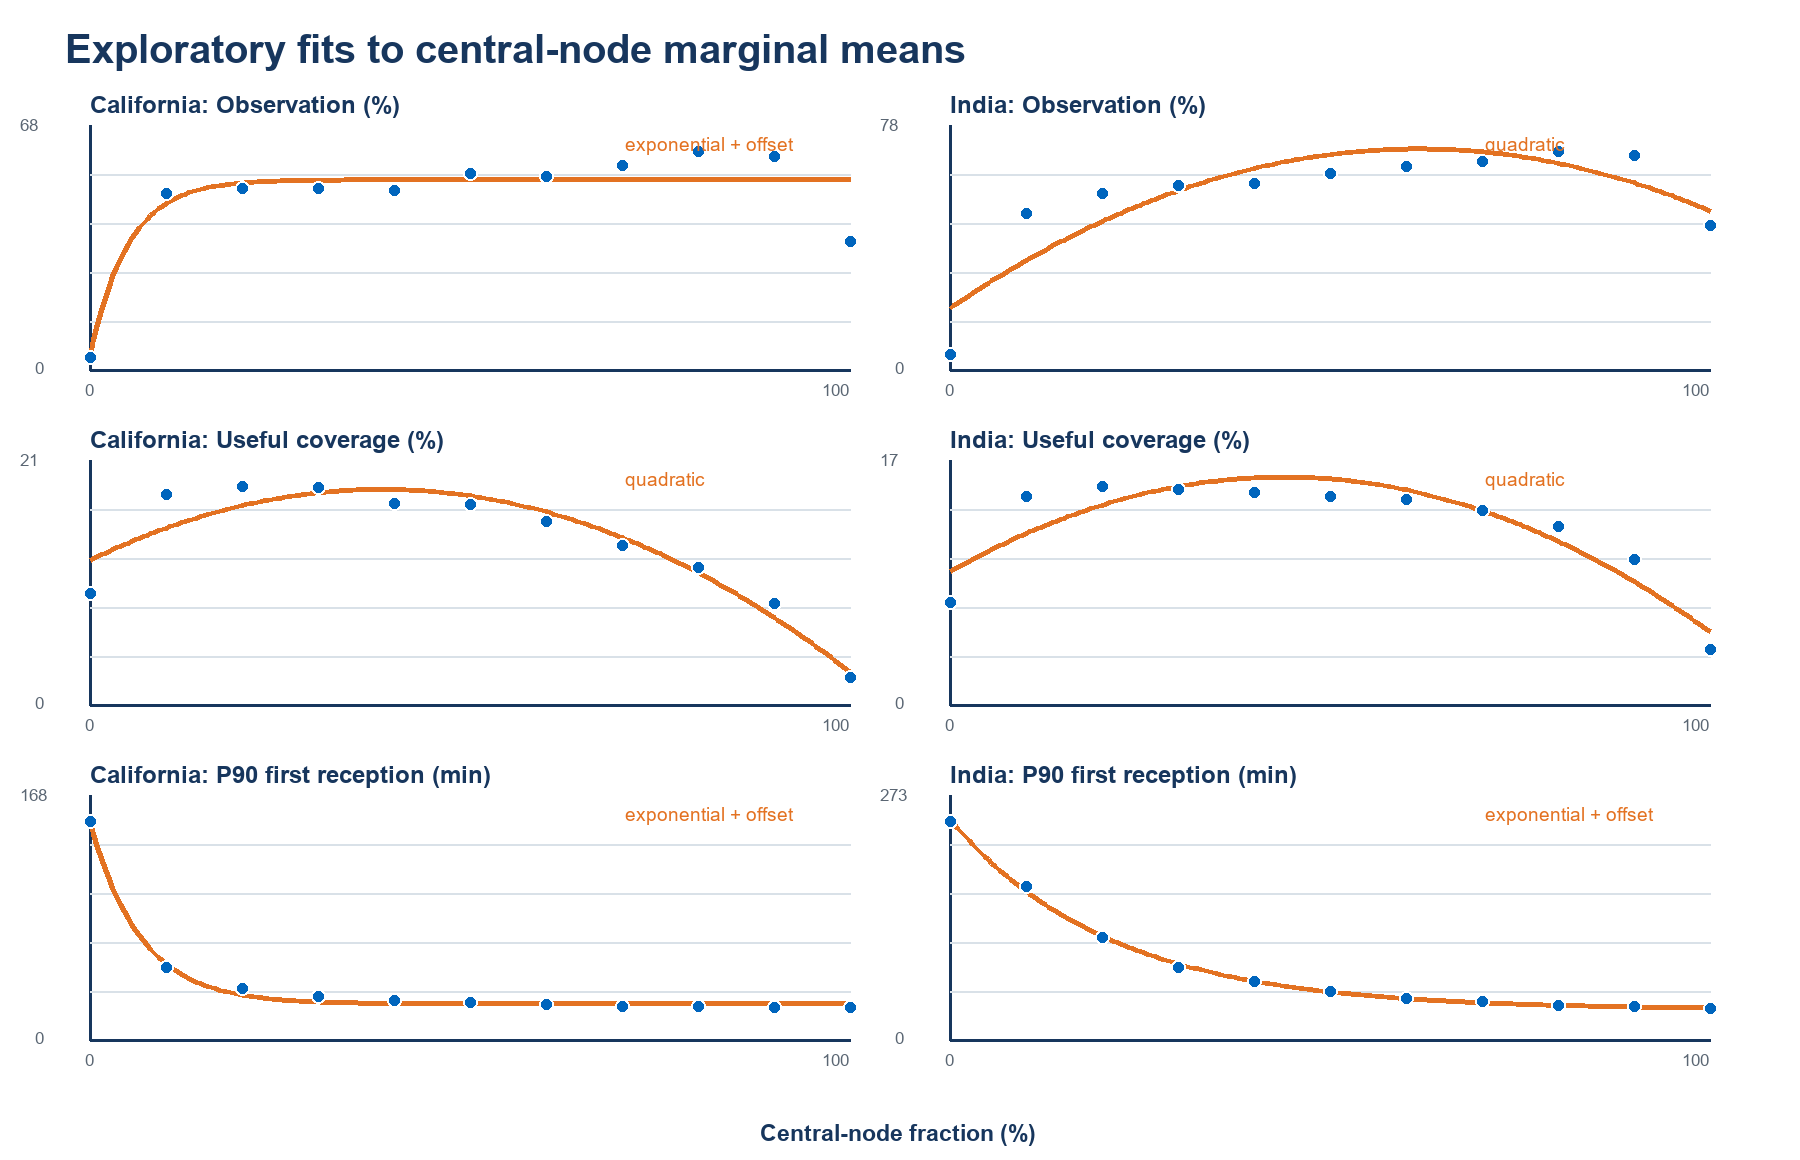
\includegraphics[width=0.98\textwidth]{regression_model_comparison.png}
\caption{Exploratory regression of the 11 regional central-node marginal means. The displayed model minimizes leave-one-level-out RMSE among linear, quadratic, cubic, and exponential-with-offset candidates.}
\label{fig:regression_models}
\end{figure}

Table~\ref{tab:regression_best} gives the selected models. California observation has a large cross-validated error despite a high in-sample $R^2$, because a saturating exponential does not reproduce the CN100 decline. This is a warning against treating the fitted curve as a physical law. India observation and both receiver responses are better represented by a quadratic over the sampled range, but extrapolation beyond 0--100 percent is meaningless.

\begin{table}[htbp]
\centering
\caption{Best exploratory regression model by leave-one-central-node-level-out error.}
\label{tab:regression_best}
\begin{tabularx}{\textwidth}{L{0.17\textwidth}Y L{0.25\textwidth}rr}
\toprule
Region & Response & Selected model & $R^2$ & LOOCV RMSE \\
\midrule
California & Observation fulfilment & Exponential + offset & 0.833 & 14.514 \\
California & Useful-receiver fraction & Quadratic & 0.911 & 2.611 \\
California & P90 first reception & Exponential + offset & 0.995 & 23.567 min \\
India & Observation fulfilment & Quadratic & 0.778 & 14.210 \\
India & Useful-receiver fraction & Quadratic & 0.851 & 2.310 \\
India & P90 first reception & Exponential + offset & 0.999 & 6.294 min \\
\bottomrule
\end{tabularx}
\end{table}

The regression result supports two qualitative conclusions. Latency benefit saturates, while receiver breadth is hump-shaped. It does not identify an optimum by itself because observation, receiver coverage, latency, and resource burden peak at different points.

\section{Paired Regional Comparison}

Figure~\ref{fig:regional_paired} compares observation fulfilment for identical architecture identifiers under the two event regions. Points above the diagonal favour India and points below favour California. The broad scatter shows that an architecture's regional performance cannot be inferred from one event alone.

\begin{figure}[htbp]
\centering
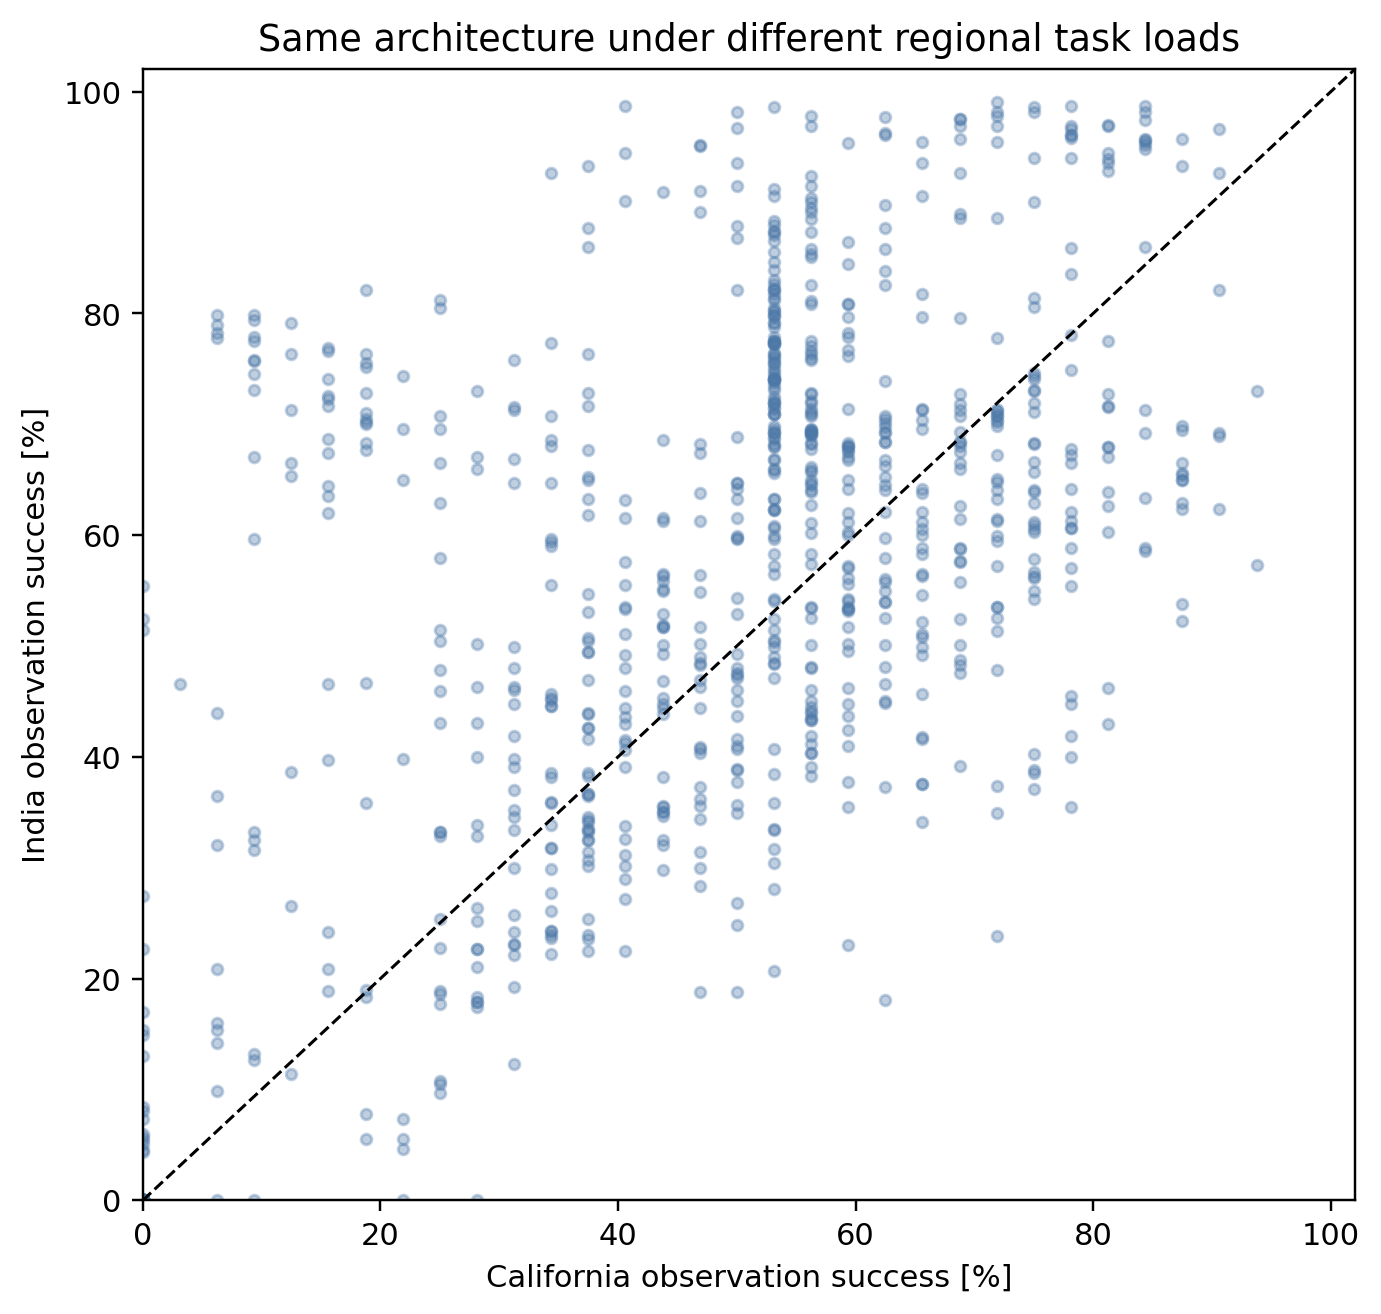
\includegraphics[width=0.72\textwidth]{04_regional_paired_observation.png}
\caption{Paired observation fulfilment for identical architecture identifiers under the California and India task sets.}
\label{fig:regional_paired}
\end{figure}

Rank agreement is reported in Table~\ref{tab:rank_agreement}. Conditional P90 first reception and receiver fraction are comparatively stable, whereas \Suseful\ ranking agreement is only 0.110. This low agreement is consistent with the different task counts, priority mixes, deadlines, and useful-recipient completion rates.

\begin{table}[htbp]
\centering
\caption{Spearman rank agreement between California and India over 891 paired architecture identifiers.}
\label{tab:rank_agreement}
\begin{tabular}{lr}
\toprule
Metric & Rank agreement \\
\midrule
Observation fulfilment & 0.504 \\
\Suseful & 0.110 \\
Mean useful-receiver fraction & 0.738 \\
Conditional P90 first-reception latency & 0.775 \\
\bottomrule
\end{tabular}
\end{table}

\section{Exact Pareto Sets}

Figure~\ref{fig:pareto} plots observation fulfilment against the declared resource-burden proxy and outlines exact Pareto members computed in the full five-objective space. A point can be Pareto optimal even if it appears dominated in this two-dimensional projection, because it may provide better \Suseful, receiver coverage, or conditional latency.

\begin{figure}[htbp]
\centering
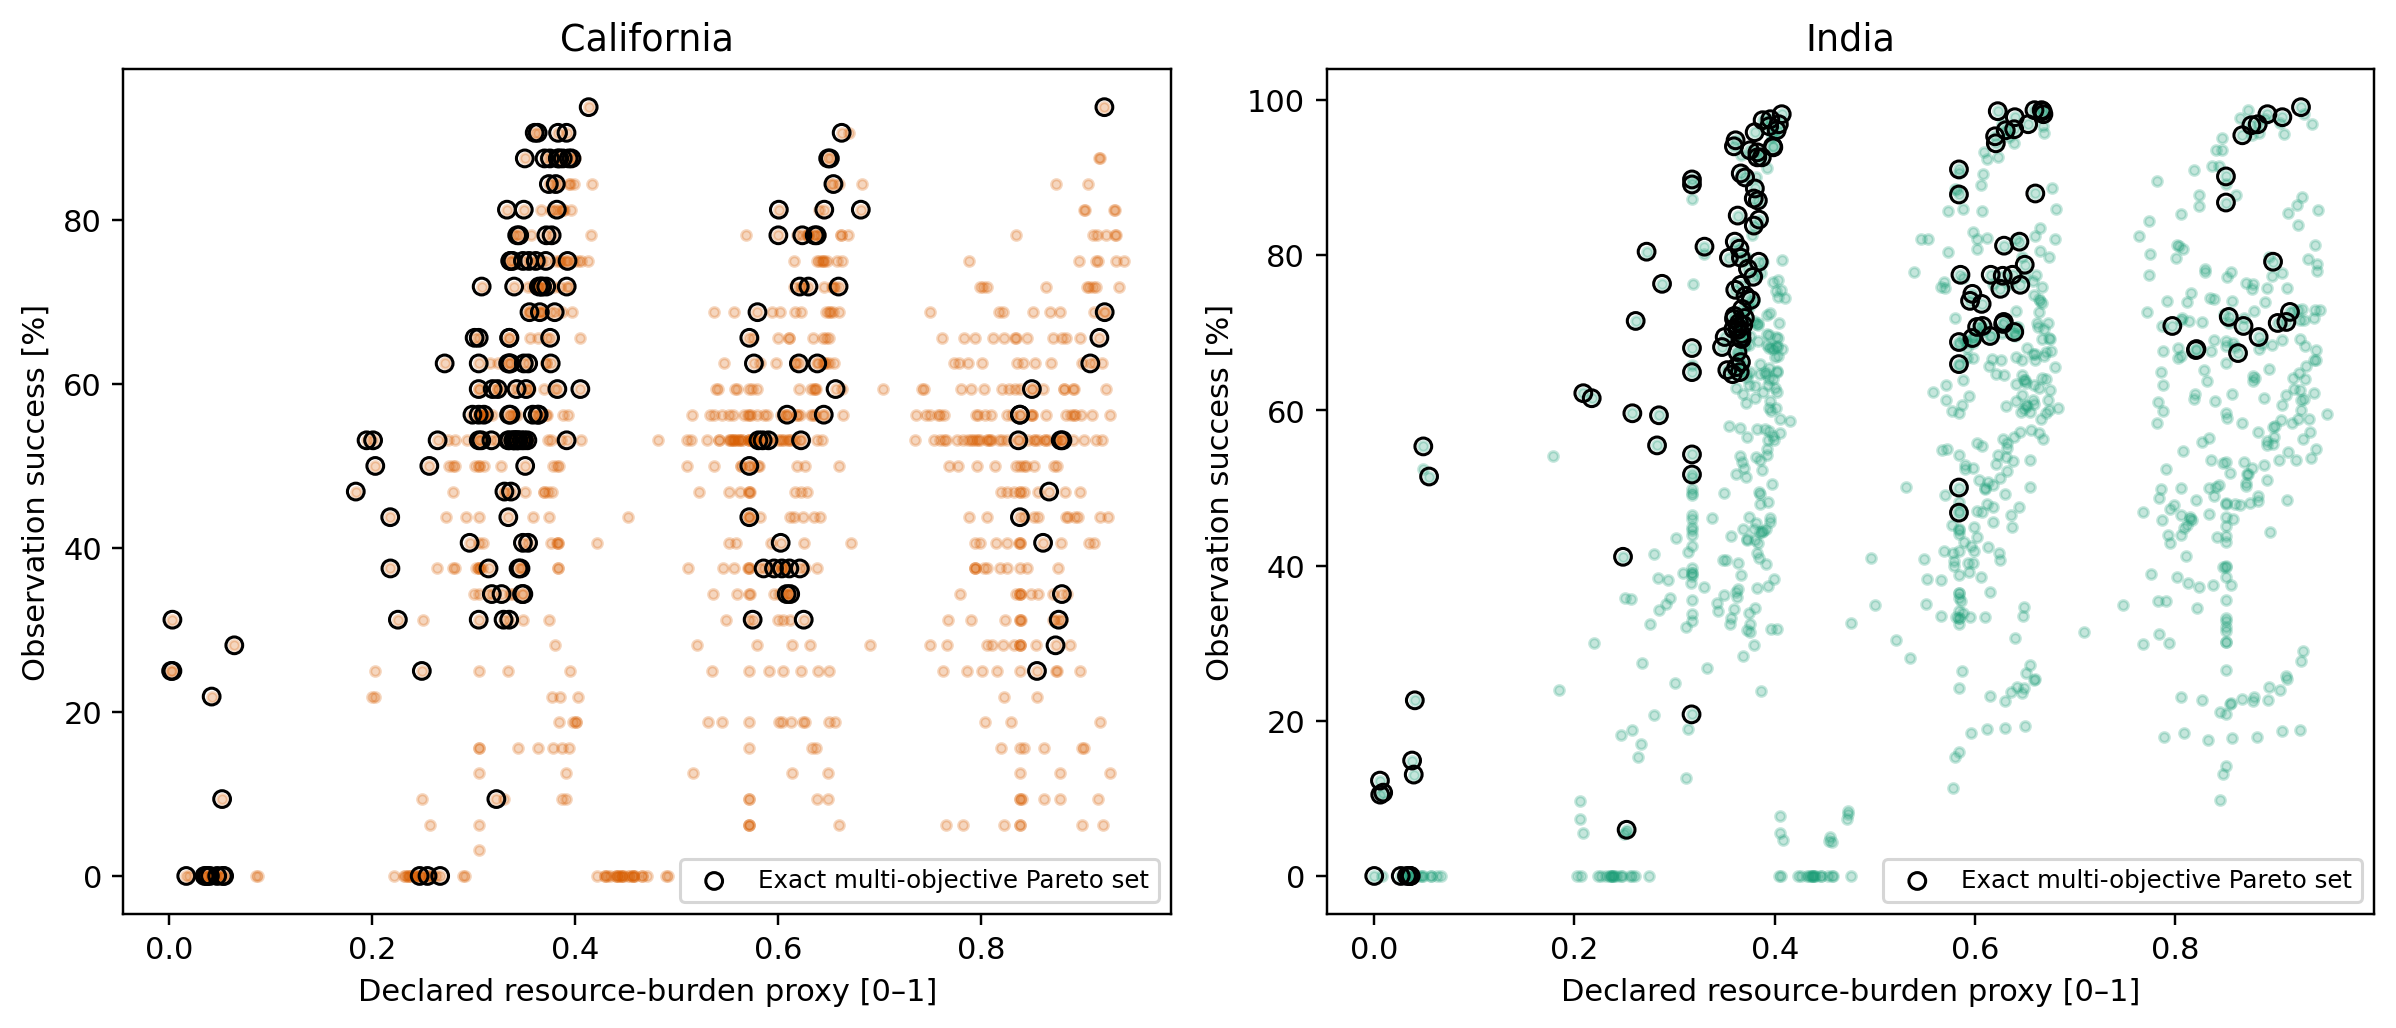
\includegraphics[width=0.98\textwidth]{02_exact_pareto_landscape.png}
\caption{Observation fulfilment versus non-monetary resource burden. Black outlines identify cases on the exact five-objective Pareto set.}
\label{fig:pareto}
\end{figure}

California has 183 Pareto cases and India has 142, corresponding to 20.5 and 15.9 percent of their candidate sets. The relatively large fronts show that the objectives are genuinely conflicting. Collapsing them into a single equal-weight score would discard viable design choices and could make the recommendation sensitive to arbitrary scaling.

\section{Nominal Result Synthesis}

The nominal campaign supports four principal findings:

\begin{enumerate}
\item introducing a modest central-node fraction produces a large improvement over CN0 in observation fulfilment and first-reception latency under the implemented central-only topology;
\item further centralization continues to reduce first-reception latency but does not monotonically improve observation, useful-recipient coverage, or \Suseful;
\item regional workload and geometry change the architecture ranking, so no winner is independent of the region; and
\item the bounded-copy, three-hop targeted policy makes rapid delivery and complete useful-recipient dissemination distinct objectives.
\end{enumerate}

These findings answer the earlier nominal centrality question but do not establish failure tolerance. Chapter~7 therefore treats robustness as a separate Fresh V2 replay and reports the validated California values independently.

\chapter{Full891 Fresh V2 California Results and Sensitivity}
\section{Scope of the Fresh V2 Results}

This chapter is the principal Fresh Full891 V2 result layer. It uses the 890 complete California architectures and, for central-node marginal curves, the 880 cases belonging to 80 complete eleven-level sweeps. The omitted case and all scenario counts are documented in Chapter~5 and Appendix~C. India Fresh V2 is not yet available; no California value in this chapter is presented as an India result.

Two scenarios anchor the interpretation. \emph{Nominal original} is the bounded central-only targeted policy with the operational deadline, three-hop limit, three observer copies, and five central-node copies. \emph{Unlimited useful deadline} removes the hop/copy limits while retaining the useful-recipient and deadline definitions. The second scenario is a diagnostic upper-capability replay, not a directly recommended operating mode.

\section{Bounded Policy versus Architecture Potential}

Table~\ref{tab:nominal_unlimited} quantifies the gap between the two anchor scenarios. Nominal mean observation fulfilment is already 61.59 percent, but strict useful-recipient completion is only 0.63 percent and mean useful coverage only 15.29 percent. Removing copy and hop limits raises strict completion to 74.69 percent and coverage to 91.14 percent. The increase requires more than ten times the transferred data.

\begin{table}[htbp]
\centering
\caption{California mean outcome over 890 complete Fresh V2 architectures.}
\label{tab:nominal_unlimited}
\begin{tabularx}{\textwidth}{L{0.28\textwidth}rrrr}
\toprule
Scenario & Obs. (\%) & \Suseful\ (\%) & Coverage (\%) & Data (Mbit/case) \\
\midrule
Nominal original & 61.59 & 0.63 & 15.29 & 197.55 \\
Unlimited useful deadline & 77.62 & 74.69 & 91.14 & 2,047.57 \\
\midrule
Difference & +16.04 & +74.07 & +75.85 & +1,850.02 \\
\bottomrule
\end{tabularx}
\end{table}

The main explanation is operational rather than purely geometric. The bounded policy frequently reaches a useful observer, which can complete the observation objective, but does not distribute the task to every useful recipient. The diagnostic replay uses additional copies and deeper temporal paths. Therefore, the low nominal \Suseful\ is a property of the architecture--policy combination, not evidence that the constellation has no communication opportunities.

\section{Central-Node Fraction}

Figure~\ref{fig:v2_cn_fraction} presents both operating regimes. Under the nominal policy, mean observation fulfilment increases sharply from 29.14 percent at CN0 to 64.88 percent at CN10, reaches 71.13 percent at CN50, and falls to 35.70 percent at CN100. Strict dissemination peaks at 1.72 percent at CN10, while mean useful coverage peaks around CN20 at approximately 20.7 percent and falls to 2.42 percent at CN100. Intermediate centralization is therefore preferable under the bounded policy.

\begin{figure}[htbp]
\centering
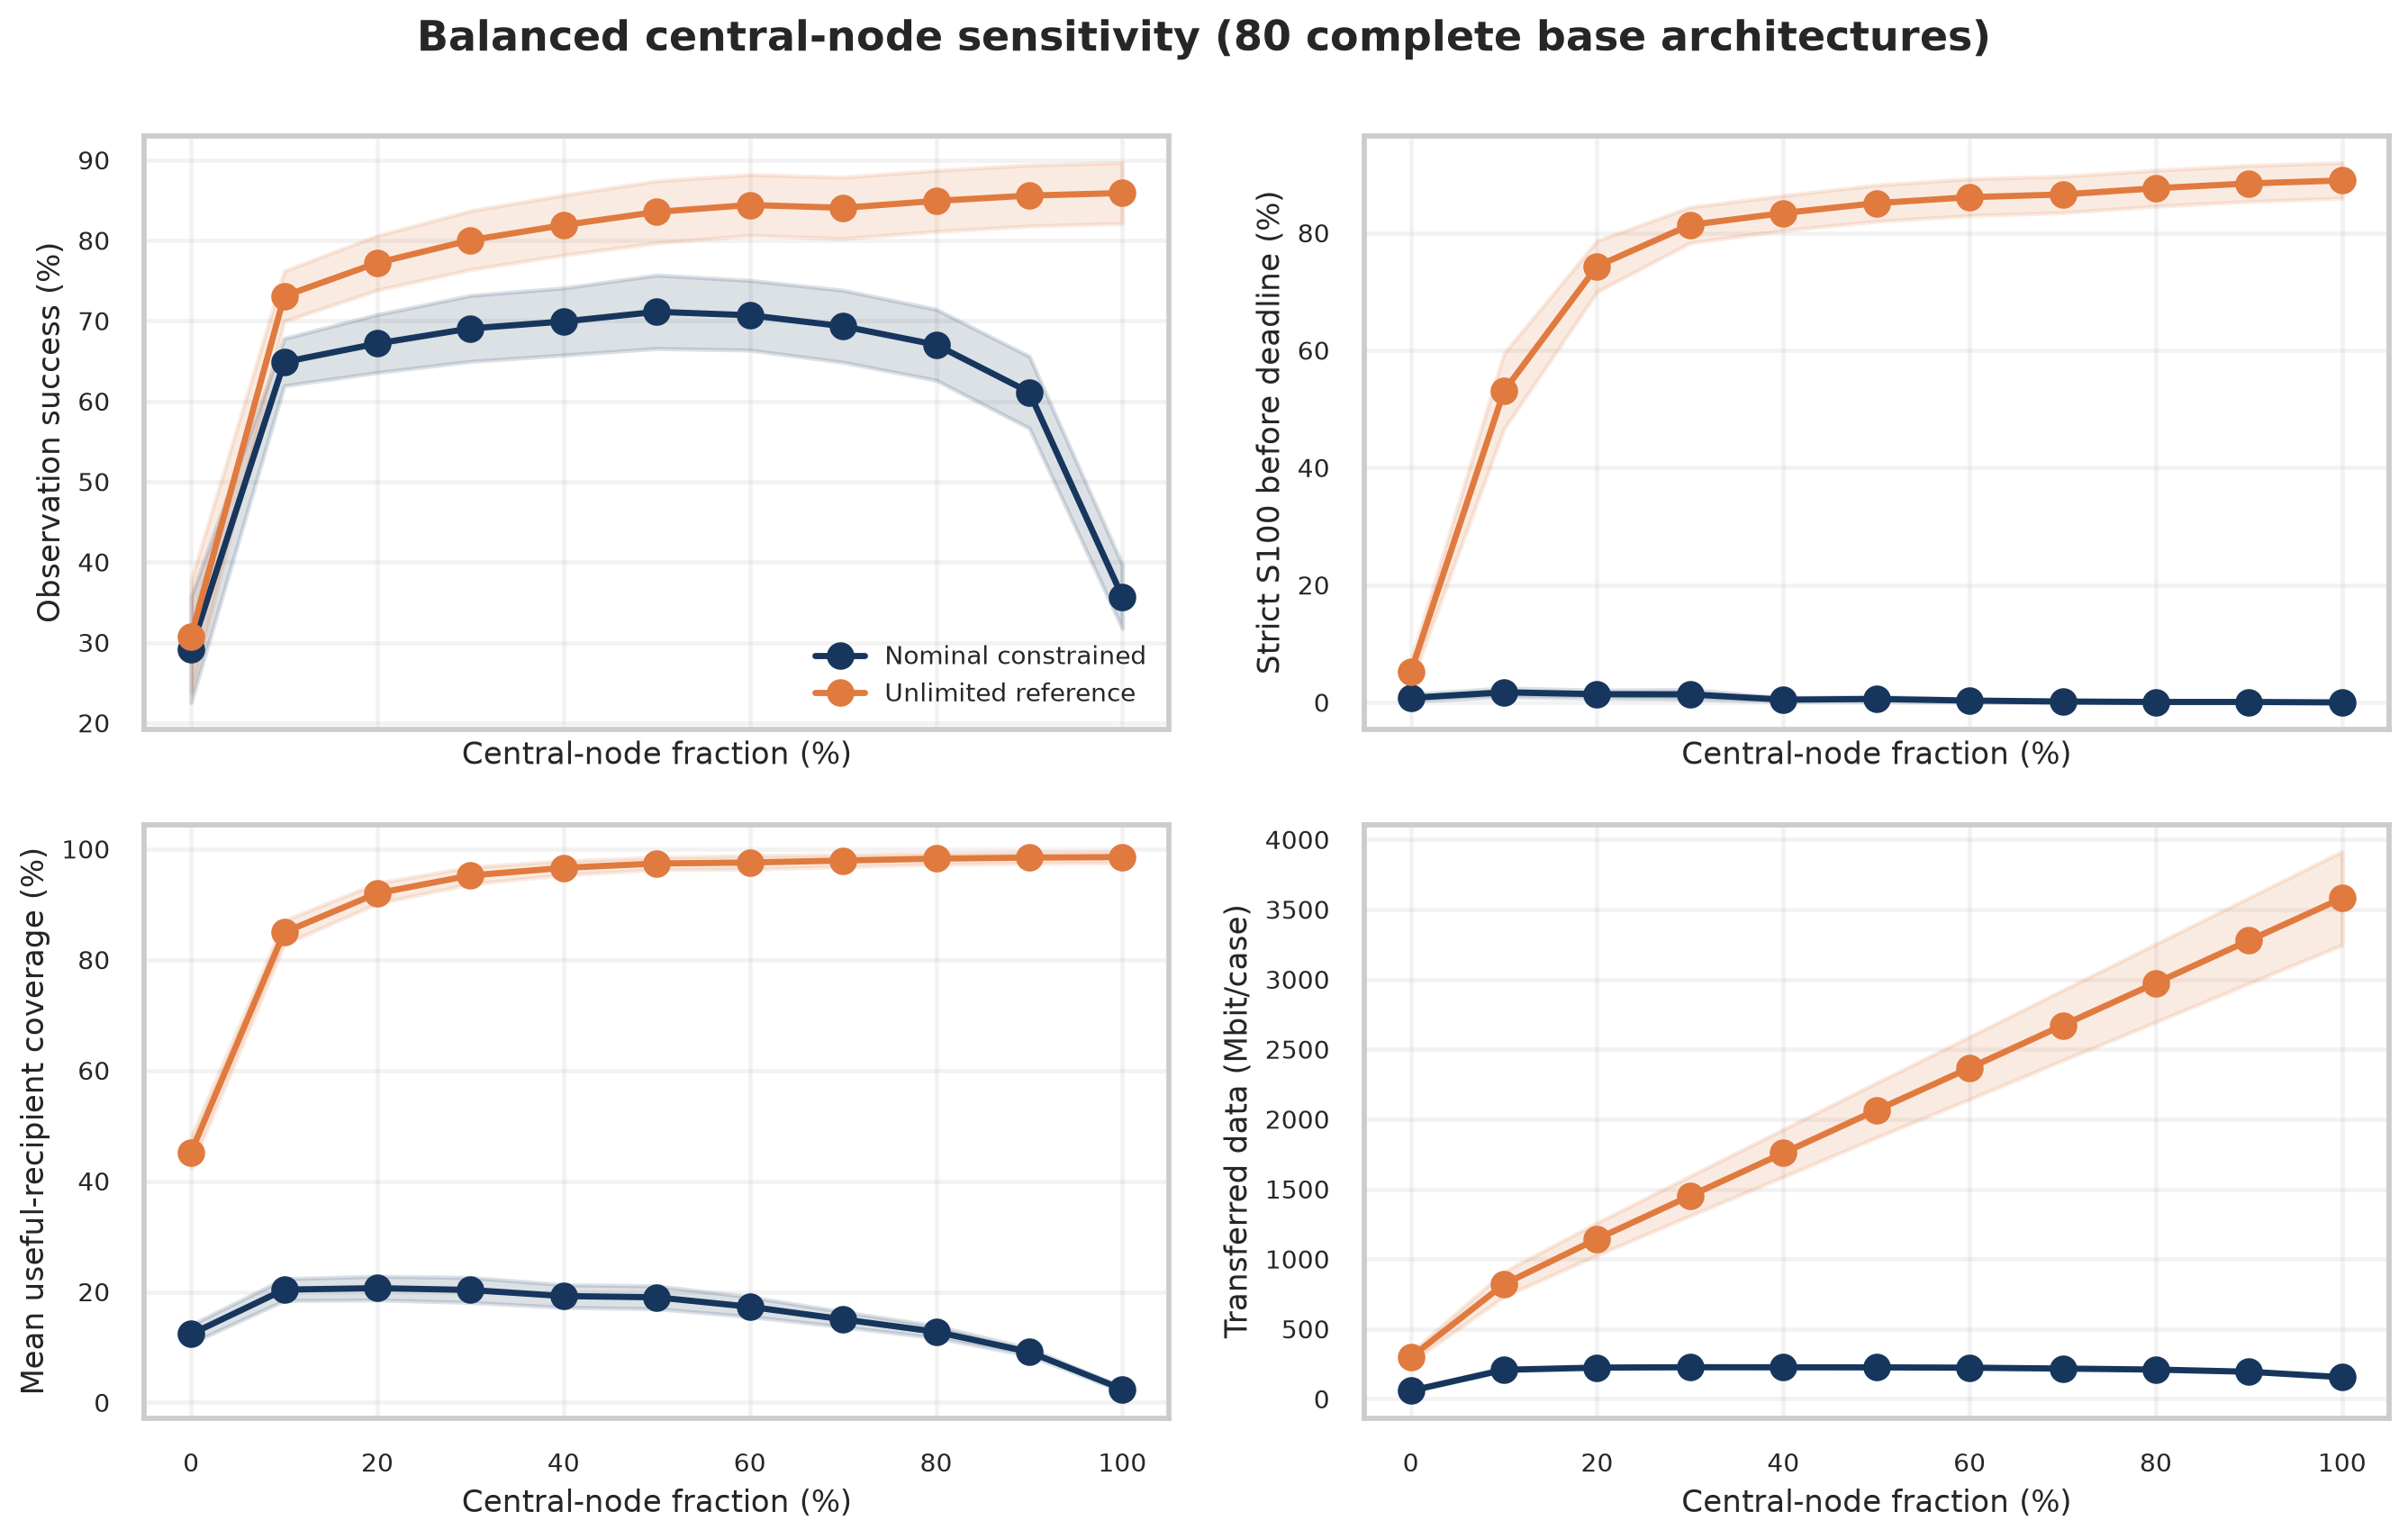
\includegraphics[width=\textwidth]{02_cn_fraction_performance.png}
\caption{Central-node fraction response across 80 balanced California Fresh V2 base architectures. Shaded or interval displays summarize variation across base geometries.}
\label{fig:v2_cn_fraction}
\end{figure}

The unlimited replay reveals a different, saturating regime. Selected marginal means are shown in Table~\ref{tab:v2_cn_selected}. \Suseful\ grows rapidly up to the intermediate range and then provides smaller incremental gains, while traffic continues to grow. From CN20 to CN100, mean \Suseful\ increases by about 14.6 points, but transferred data increases by approximately 2,429 Mbit per case (about 211 percent).

\begin{table}[htbp]
\centering
\caption{Selected unlimited useful-deadline central-node marginal means.}
\label{tab:v2_cn_selected}
\begin{tabular}{rrrrrr}
\toprule
CN (\%) & \Suseful\ (\%) & Coverage (\%) & P100 $T_{100}$ (min) & Data (Mbit) & Events \\
\midrule
0 & 5.16 & 45.21 & 232.6 & 297 & 407 \\
20 & 74.34 & 92.02 & 120.0 & 1,152 & 1,333 \\
40 & 83.40 & 96.61 & 97.4 & 1,771 & 1,939 \\
70 & 86.56 & -- & -- & -- & -- \\
100 & 88.95 & 98.55 & 73.2 & 3,581 & 3,709 \\
\bottomrule
\end{tabular}
\end{table}

The dashes denote values not selected for the compact table; they are not treated as zero. P100 $T_{100}$ is conditional and especially censored at CN0. In the nominal scenario, mean maximum routing depth reaches the configured limit of three by approximately CN20. In the unlimited replay it rises from 1.0 at CN0 to about 7.8 at CN20, 9.6 at CN40, and 11.8 at CN100. Part of the unlimited gain is therefore attributable to policy freedom, not central-node fraction alone.

\section{Architecture Factors and Dependence}

Figure~\ref{fig:v2_arch_effects} shows descriptive main effects. Within the unlimited balanced subset, unadjusted one-factor $\eta^2$ for CN fraction is 0.690 for \Suseful\ and 0.820 for useful coverage. Plane count is the next largest reported factor for \Suseful\ at 0.112. For observation fulfilment, CN fraction and plane count have $\eta^2$ values of 0.402 and 0.361. Satellite count, altitude, and inclination are smaller in these marginal summaries.

\begin{figure}[htbp]
\centering
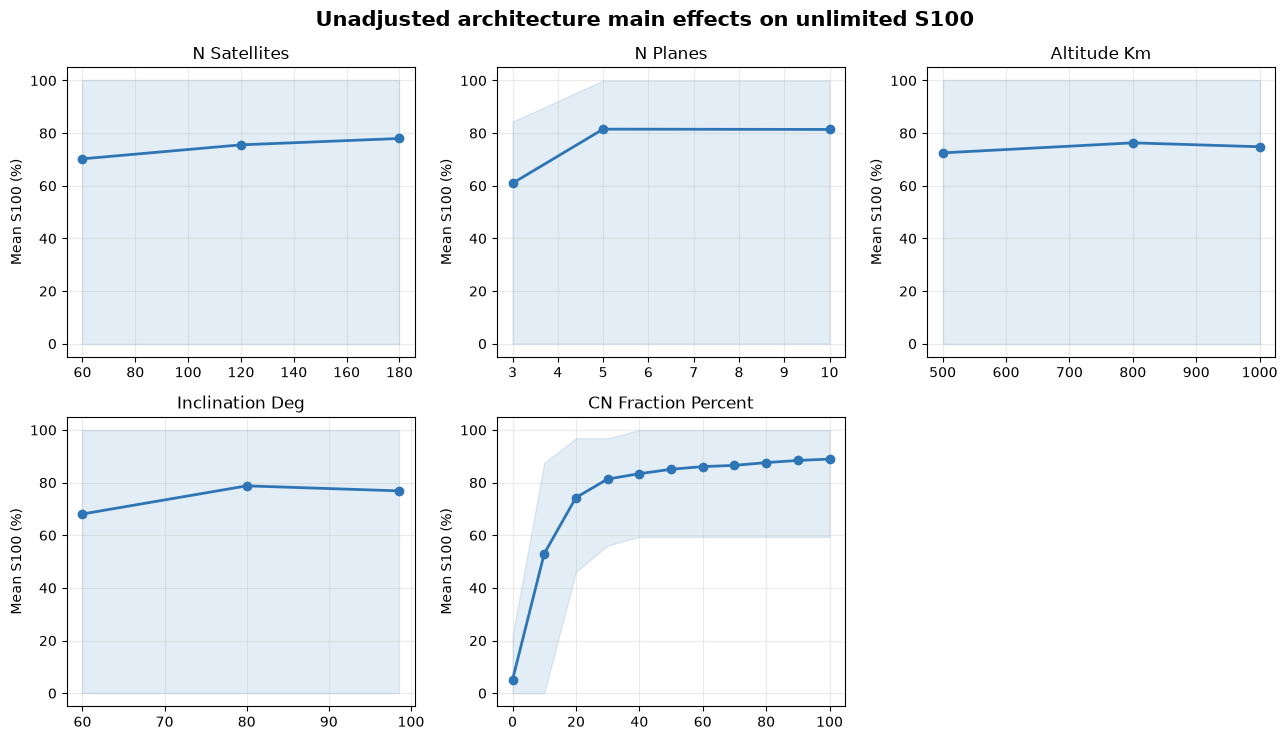
\includegraphics[width=\textwidth]{03_architecture_main_effects.png}
\caption{California Fresh V2 marginal architecture effects under the unlimited useful-deadline replay.}
\label{fig:v2_arch_effects}
\end{figure}

These values show that dissemination depends strongly on the central-node role, while observation also depends materially on plane geometry. Because the design contains interactions and discrete placement changes, the unadjusted effects are descriptive. They do not imply that changing one factor while holding an unmodelled system fixed will reproduce the marginal mean.

\section{Policy Ablation}

The policy ablation in Table~\ref{tab:policy_ablation} separates central-only access from all-peer link availability. Peer-only and hybrid produce identical recorded outcomes in the current implementation. This identity is important: it indicates that the implemented hybrid preference does not change admitted transfers relative to peer-only for this scenario set. It is not evidence that every possible hybrid algorithm is equivalent to peer routing.

\begin{table}[htbp]
\centering
\caption{Mean California policy-ablation outcome over 890 complete architectures.}
\label{tab:policy_ablation}
\begin{tabular}{lrrrr}
\toprule
Policy scenario & Obs. (\%) & \Suseful\ (\%) & Coverage (\%) & Data (Mbit/case) \\
\midrule
Central / unlimited & 77.62 & 74.69 & 91.14 & 2,047.57 \\
Peer & 83.04 & 85.44 & 97.20 & 3,485.72 \\
Hybrid & 83.04 & 85.44 & 97.20 & 3,485.72 \\
\bottomrule
\end{tabular}
\end{table}

\begin{figure}[htbp]
\centering
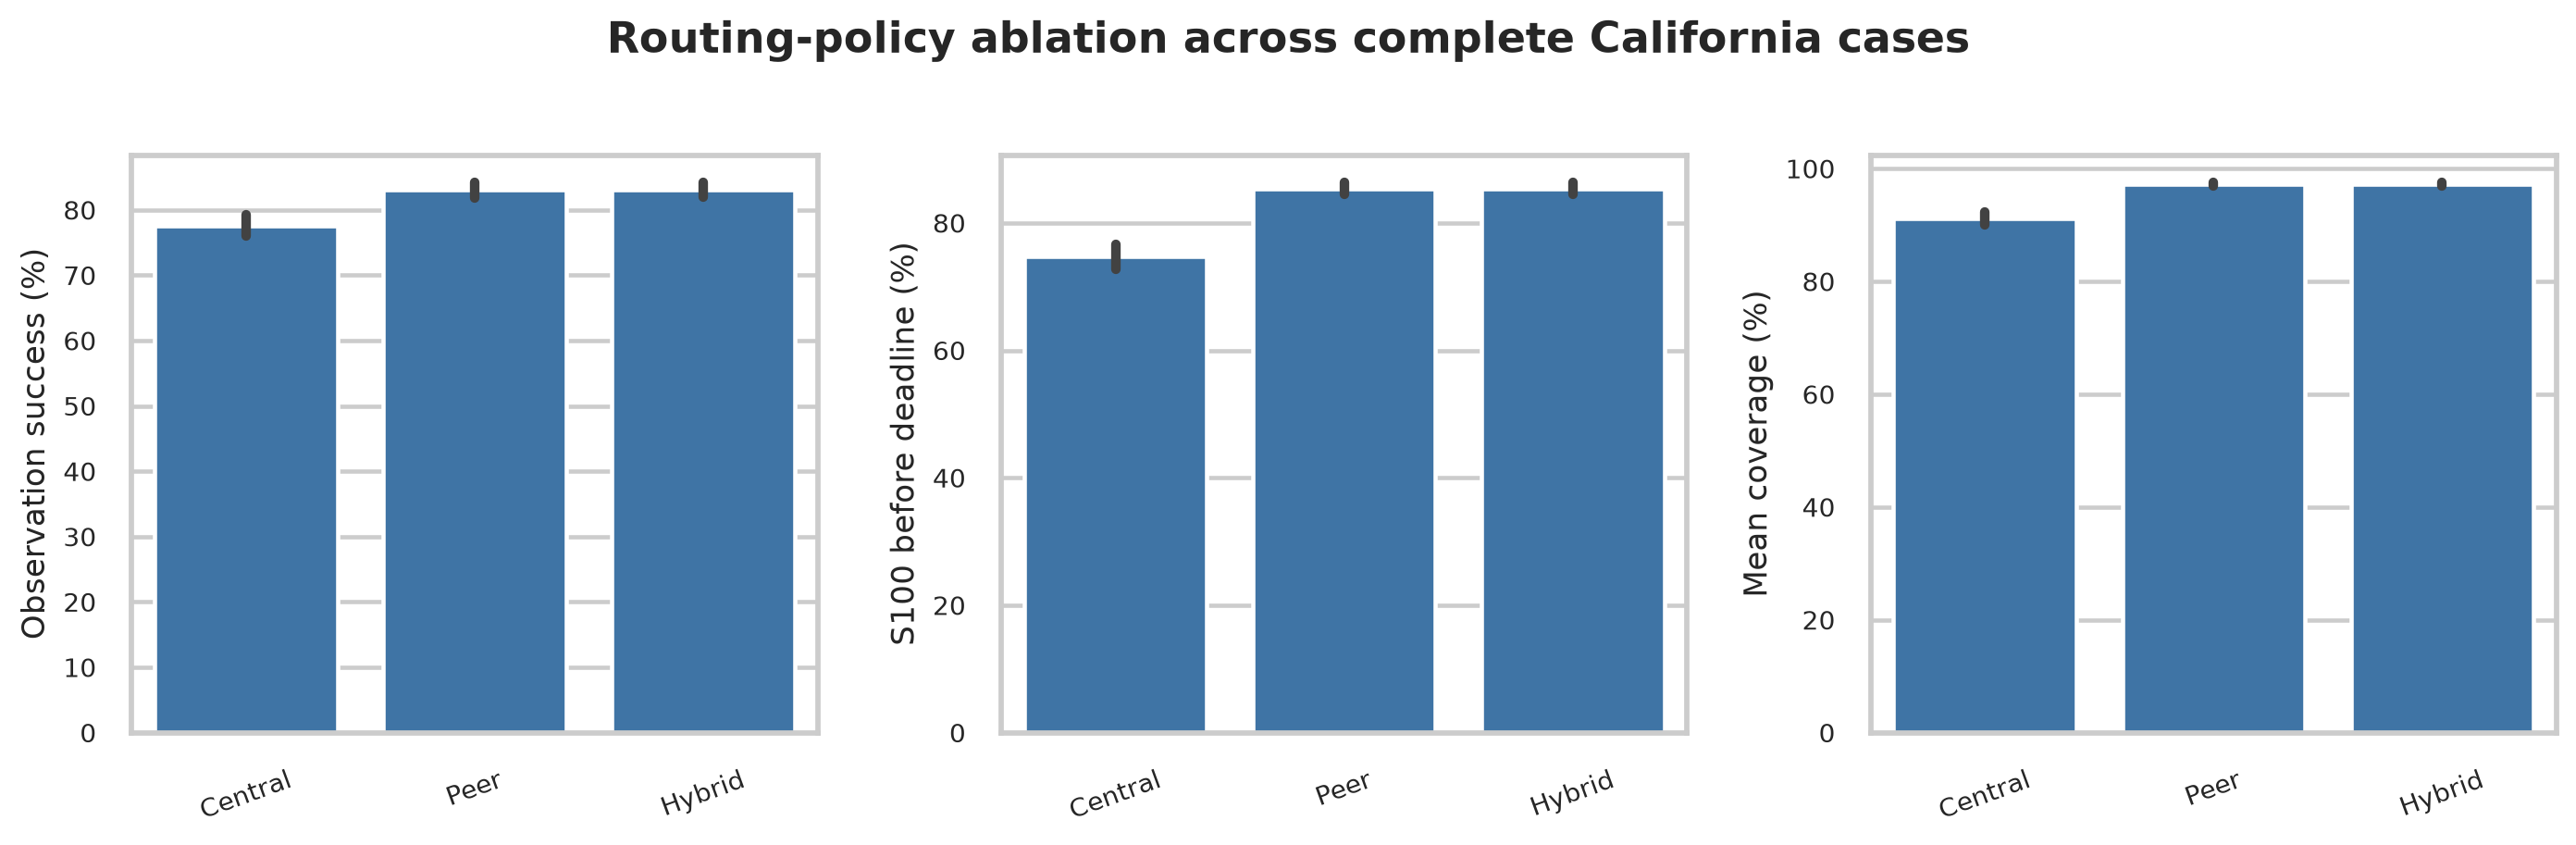
\includegraphics[width=0.92\textwidth]{04_policy_ablation.png}
\caption{Policy ablation: performance gain and communication burden under central, peer, and hybrid link use.}
\label{fig:policy_ablation}
\end{figure}

The peer-capable variants improve observation by 5.42 percentage points and \Suseful\ by 10.75 points relative to central-only unlimited routing, but increase mean transferred data by approximately 1,438 Mbit per case. The comparison demonstrates that link availability and central-node fraction must be interpreted jointly.

\section{Task-Size Sensitivity}

Task-size scaling provides a direct communication-load stress test while retaining the same tasks and physical opportunities. Table~\ref{tab:task_size} and Figure~\ref{fig:task_size} show monotonic degradation as packets grow. Halving the packet size slightly improves performance and approximately halves traffic; quadrupling it reduces observation fulfilment by 8.14 points and strict completion by 14.59 points relative to the 1$\times$ case.

\begin{table}[htbp]
\centering
\caption{California task-size sensitivity over 890 complete architectures.}
\label{tab:task_size}
\begin{tabular}{rrrrr}
\toprule
Multiplier & Obs. (\%) & \Suseful\ (\%) & Coverage (\%) & Data (Mbit/case) \\
\midrule
0.5$\times$ & 79.33 & 76.01 & 91.72 & 1,036.55 \\
1$\times$ & 77.62 & 74.69 & 91.14 & 2,047.57 \\
2$\times$ & 75.12 & 71.73 & 89.38 & 3,979.20 \\
4$\times$ & 69.48 & 60.10 & 82.36 & 7,219.41 \\
\bottomrule
\end{tabular}
\end{table}

\begin{figure}[htbp]
\centering
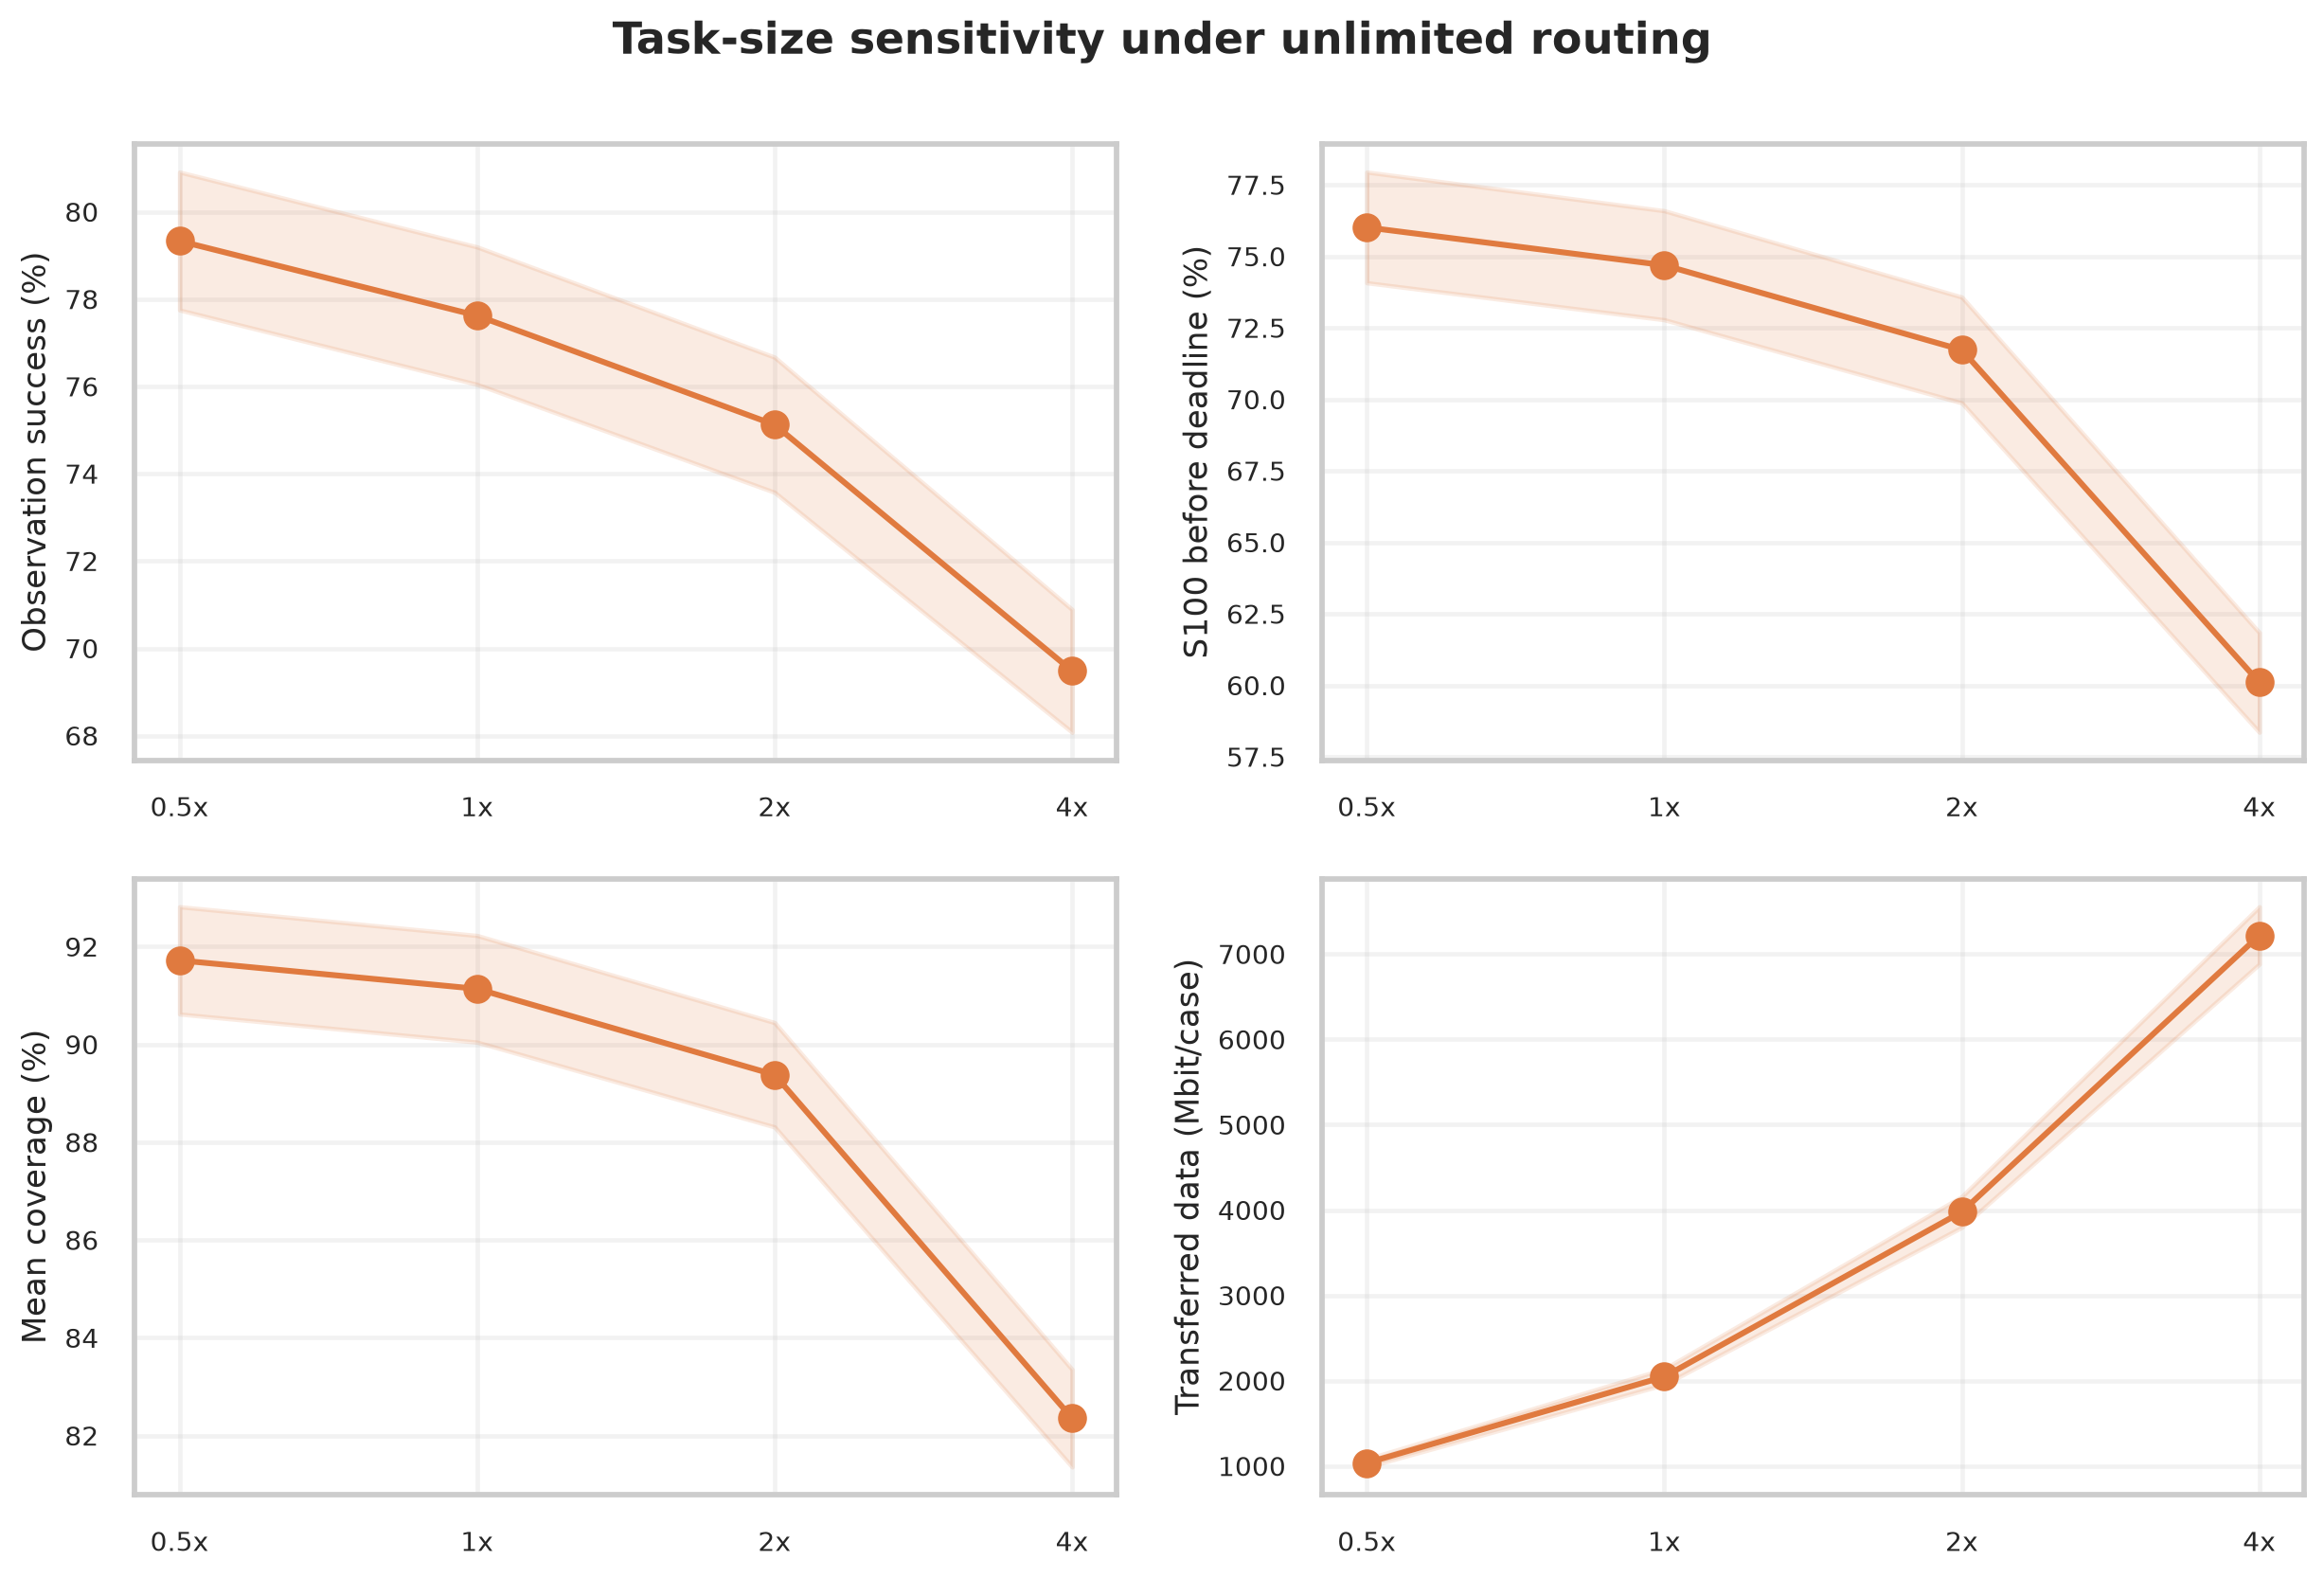
\includegraphics[width=\textwidth]{05_task_size_sensitivity.png}
\caption{Task-size sensitivity of performance and communication burden.}
\label{fig:task_size}
\end{figure}

The balanced 40-percent-CN candidate retains 96.875 percent observation at 2$\times$ size but falls to 87.5 percent at 4$\times$; its \Suseful\ changes from 100 percent at 1$\times$ to 96.875 and 78.125 percent. A recommendation based on small task descriptions is therefore not invariant to heavier products.

\section{Priority-Class Outcomes}

California contains one Critical, six High, sixteen Medium, and nine Low tasks. Figure~\ref{fig:priority_outcomes} shows that urgent classes are substantially harder under both anchor scenarios. The nominal mean observation outcomes are 8.20, 23.09, 63.43, and 89.90 percent for Critical through Low. Under the unlimited replay they become 29.21, 53.75, 79.66, and 95.31 percent. Corresponding unlimited \Suseful\ means are 24.49, 54.55, 77.80, and 88.16 percent.

\begin{figure}[htbp]
\centering
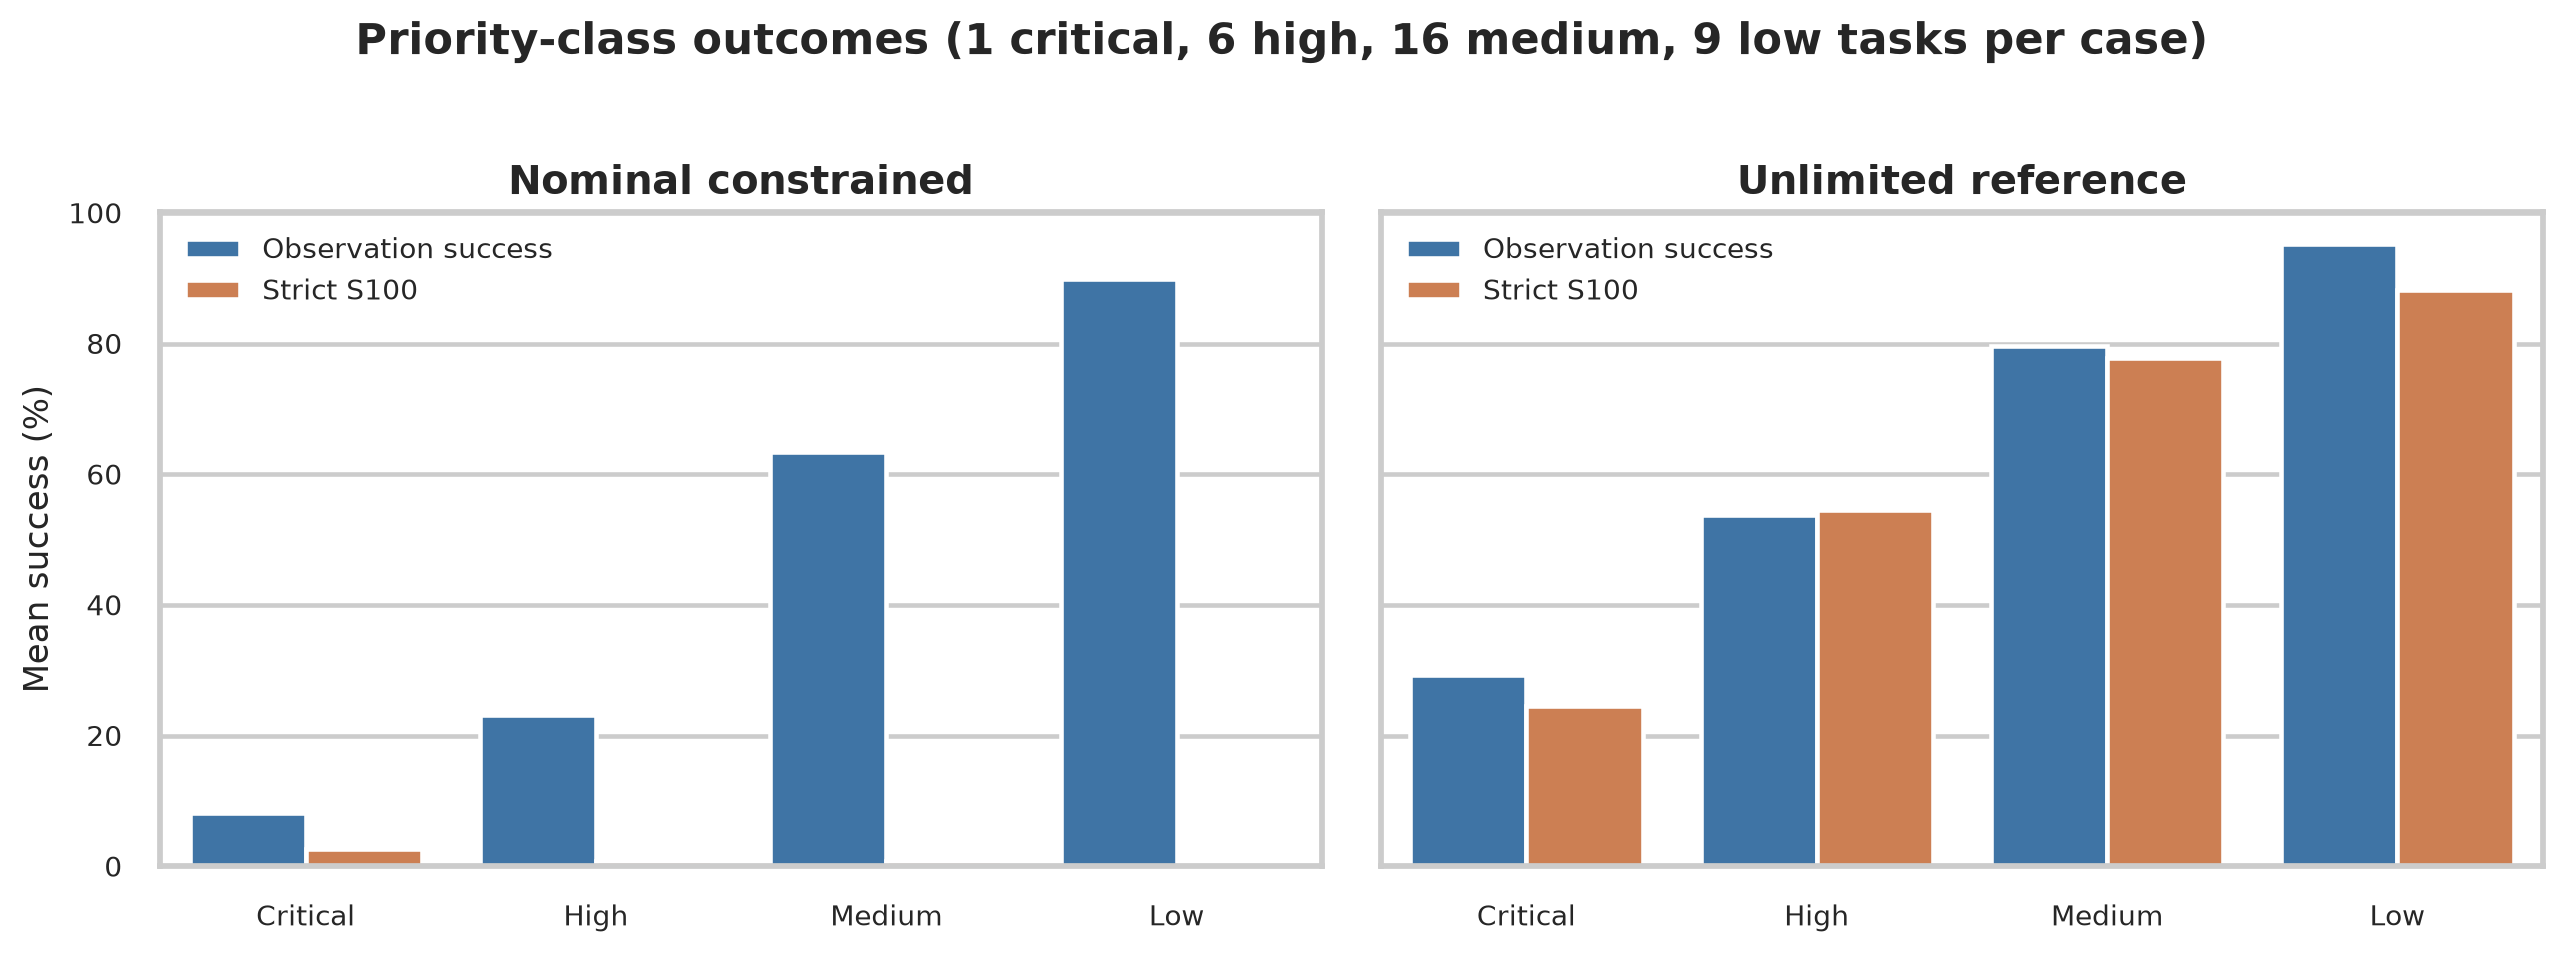
\includegraphics[width=0.92\textwidth]{07_priority_outcomes.png}
\caption{California task-priority outcomes under nominal and unlimited scenarios.}
\label{fig:priority_outcomes}
\end{figure}

This pattern does not isolate a causal priority effect. Priority is jointly encoded through deadline and message size, and each class contains different task locations and release times. The Critical class has one task. The result supports a workload-heterogeneity conclusion, not a general claim that high-FRP fires are intrinsically harder to observe.

\section{Failure Robustness}

For failure scenarios, each architecture is compared with its own unlimited baseline. Table~\ref{tab:robustness_30} reports the average percentage-point effect at the 30-percent level. Ground-station outage is the dominant tested stressor. Satellite and central-node failure produce moderate average losses; capacity degradation is smaller at the tested level.

\begin{table}[htbp]
\centering
\caption{Mean paired performance change at the 30-percent stress level.}
\label{tab:robustness_30}
\begin{tabularx}{\textwidth}{L{0.40\textwidth}rrY}
\toprule
Failure family & $\Delta$ Obs. (pp) & $\Delta$ \Suseful\ (pp) & Interpretation \\
\midrule
Ground-station outage & $-21.46$ & $-20.84$ & Dominant tested vulnerability \\
Targeted central-node failure & $-2.95$ & $-6.57$ & Larger dissemination than observation penalty \\
Random central-node failure & $-2.86$ & $-5.98$ & Moderate mean loss \\
Random satellite failure & $-3.01$ & $-3.91$ & Geometry and forwarding loss \\
Capacity degradation & $< -1$ & approximately $-1$ & Small at tested severity \\
\bottomrule
\end{tabularx}
\end{table}

\begin{figure}[htbp]
\centering
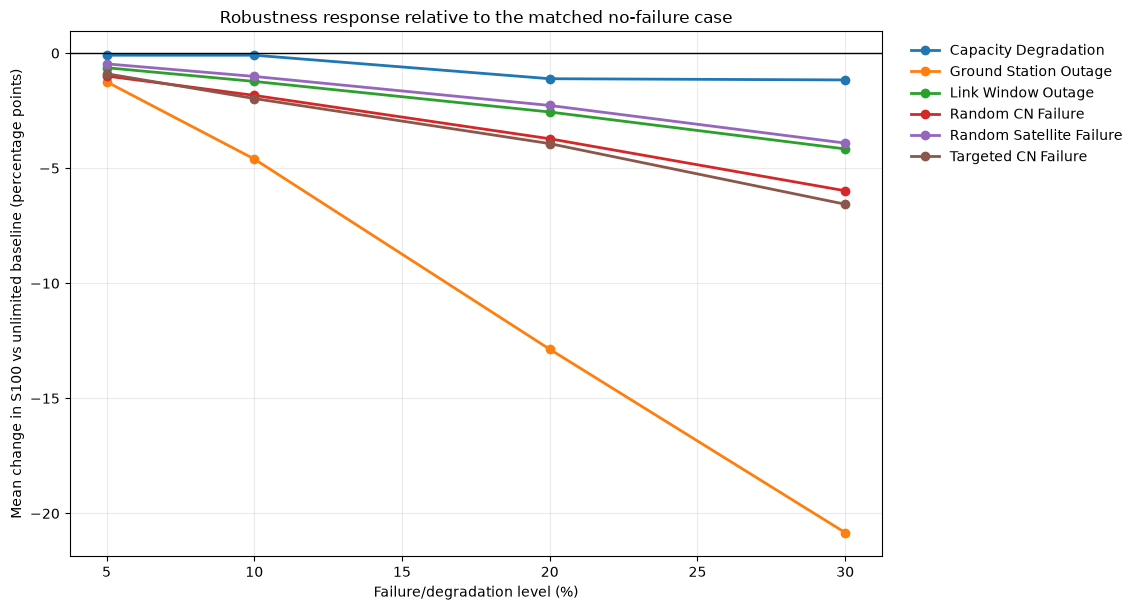
\includegraphics[width=\textwidth]{06_robustness_delta_s100.png}
\caption{Paired change in strict useful dissemination across Fresh V2 robustness families and severities.}
\label{fig:robustness_s100}
\end{figure}

For the balanced candidate \texttt{T060\_P10\_H0800\_I0986\_CN040\_F1}, the unlimited baseline is 96.875 percent observation and 100 percent \Suseful. At 30-percent random central-node failure, replicate means are 91.25 and 93.75 percent; at 30-percent random satellite failure they are 92.08 and 95.52 percent. Deterministic targeted-CN failure retains 93.75 percent observation and 100 percent \Suseful, although P100 $T_{100}$ increases from 66.10 to 124.42 minutes. Ground-station-outage replicate means fall to 66.77 and 69.79 percent. Ground diversity is therefore a more direct design need than simply raising the central-node fraction beyond the intermediate range.

\section{Pareto Trade Space}

No architecture dominates all others on performance and burden. Figure~\ref{fig:v2_pareto} shows the unlimited trade space. The original six-objective analysis---observation, \Suseful, useful coverage, satellites, central nodes, and transferred data---contains 48 exact Pareto cases. Adding P100 $T_{100}$ and transfer-event count for consistency with the utility definition produces an eight-objective frontier of 108 cases; all original 48 remain efficient.

\begin{figure}[htbp]
\centering
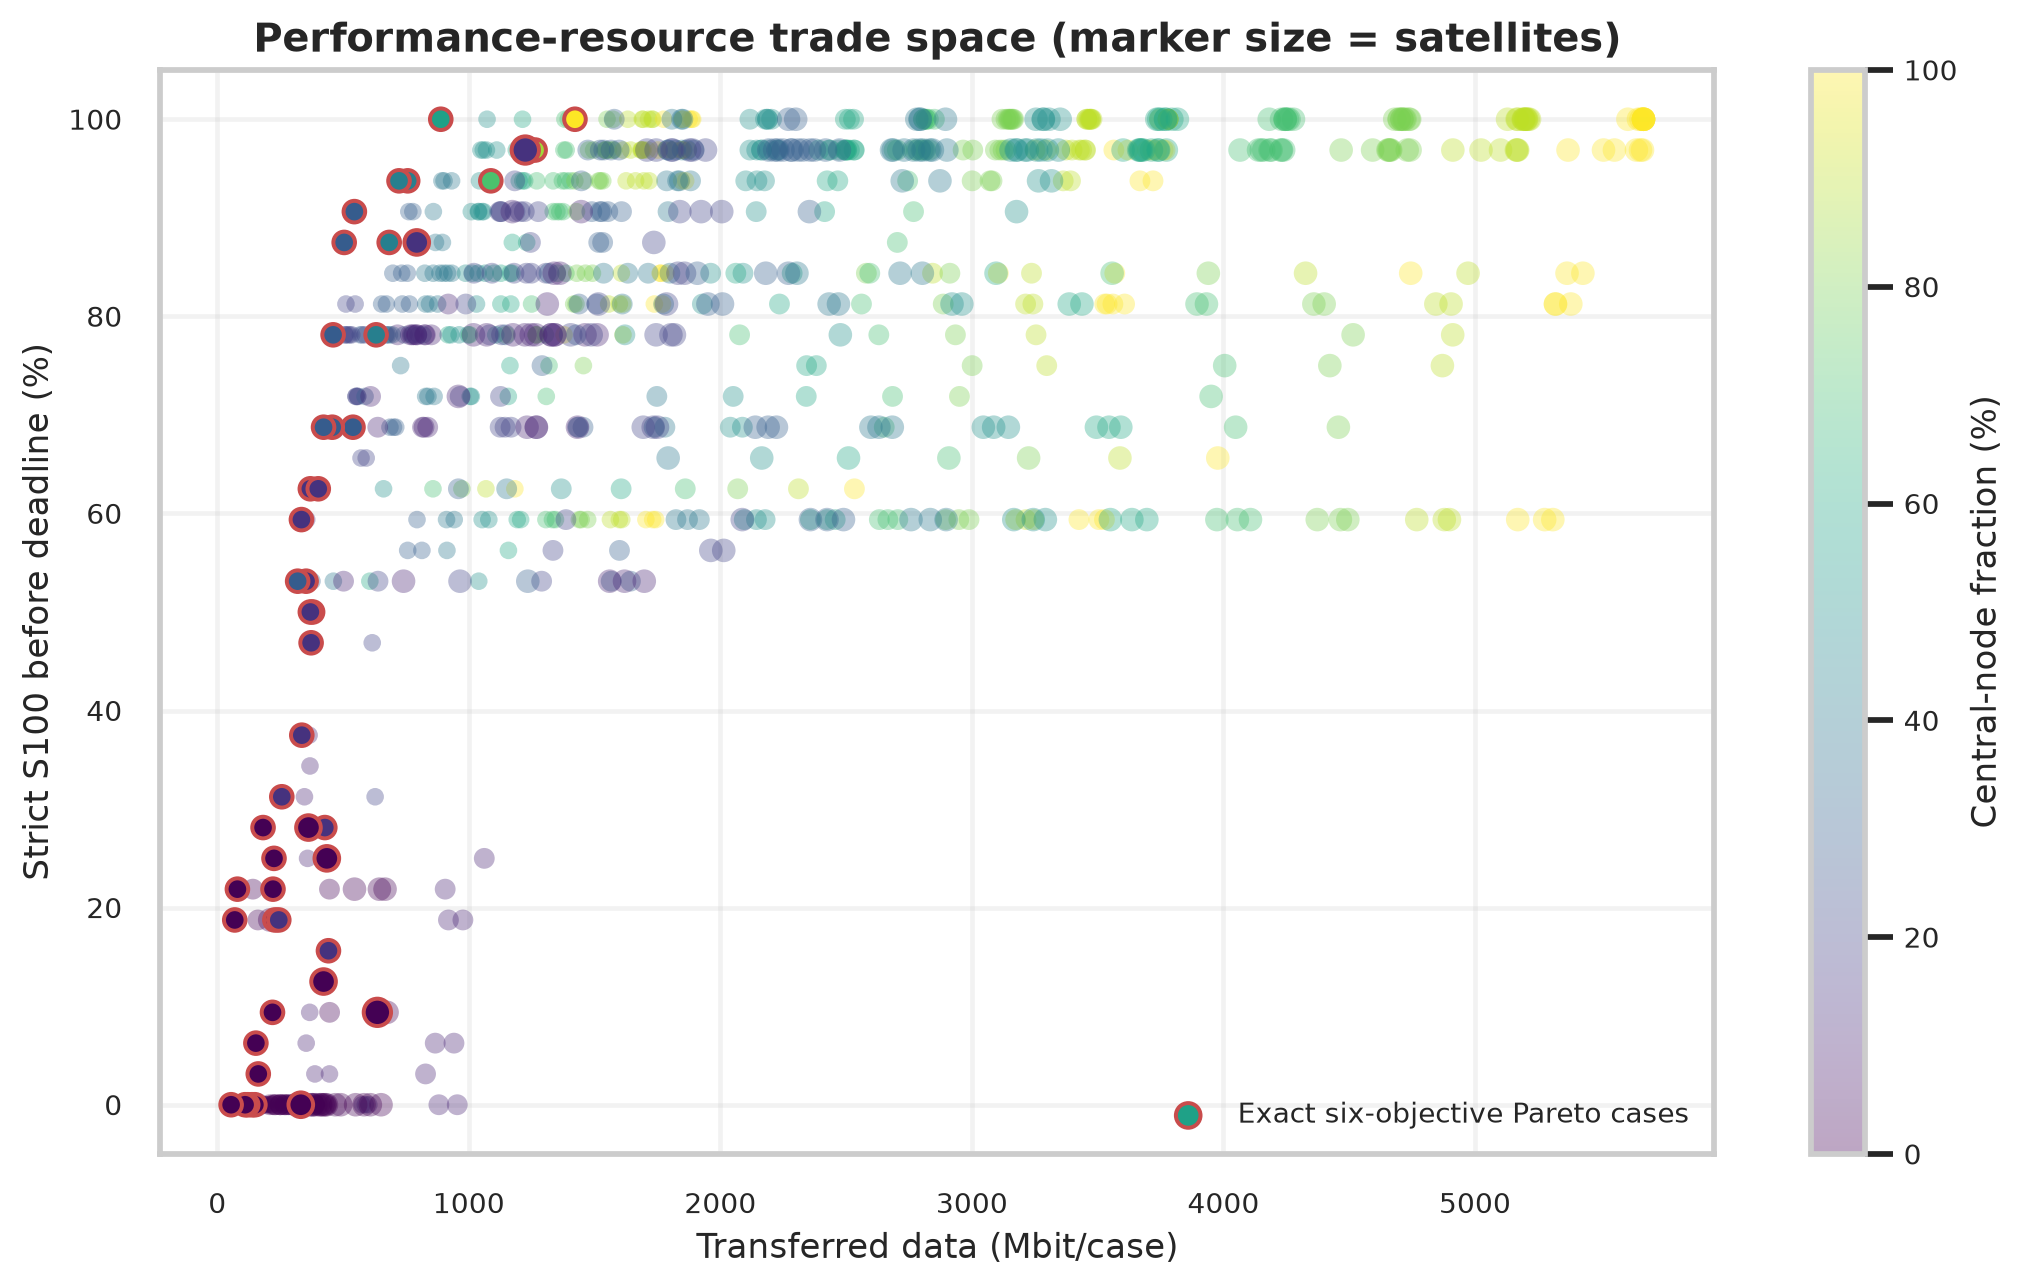
\includegraphics[width=\textwidth]{09_unlimited_pareto_trade_space.png}
\caption{California unlimited performance--resource trade space and exact Pareto membership.}
\label{fig:v2_pareto}
\end{figure}

Table~\ref{tab:decision_cases} gives three transparent decision points. The balanced candidate achieves complete useful dissemination and coverage with 60 satellites and less than one-sixth of the transferred data of the fastest perfect-performance extreme.

\begin{table}[htbp]
\centering
\small
\caption{Illustrative California Fresh V2 Pareto candidates.}
\label{tab:decision_cases}
\begin{tabularx}{\textwidth}{L{0.31\textwidth}rrrrr}
\toprule
Case & Obs. (\%) & \Suseful\ (\%) & Cov. (\%) & P100 $T_{100}$ (min) & Mbit \\
\midrule
\shortstack[l]{\texttt{T060\_P10\_H0800}\protect\\\texttt{I0986\_CN040\_F1}} & 96.875 & 100 & 100 & 66.10 & 888.5 \\
\shortstack[l]{\texttt{T060\_P05\_H0800}\protect\\\texttt{I0800\_CN070\_F1}} & 100 & 100 & 100 & 56.20 & 1,422 \\
\shortstack[l]{\texttt{T180\_P10\_H0800}\protect\\\texttt{I0800\_CN100\_F1}} & 100 & 100 & 100 & 33.59 & 5,670 \\
\bottomrule
\end{tabularx}
\end{table}

The first case has 24 central nodes; the second has 42; the third has 180. The first is the recommended California compromise under the declared balanced weighting, not a universal optimum or a cost-optimal spacecraft design.

\section{Objective-Weight Analysis}

The weight analysis introduces preference only after exact Pareto screening and normalization over all 890 complete cases. Table~\ref{tab:weight_profiles} shows three declared high-level profiles. Cost-dominant is shorthand for resource-dominant; the score is non-monetary.

\begin{table}[htbp]
\centering
\caption{Declared weight profiles and selected California architecture.}
\label{tab:weight_profiles}
\begin{tabularx}{\textwidth}{L{0.20\textwidth}rrY}
\toprule
Profile & Performance & Resource & Winner \\
\midrule
Resource-dominant & 0.25 & 0.75 & \texttt{T060\_P05\_H1000\_I0986\_CN030\_F1} \\
Balanced & 0.50 & 0.50 & \texttt{T060\_P10\_H0800\_I0986\_CN040\_F1} \\
Performance-dominant & 0.75 & 0.25 & \texttt{T060\_P10\_H0800\_I0986\_CN040\_F1} \\
\bottomrule
\end{tabularx}
\end{table}

\begin{figure}[htbp]
\centering
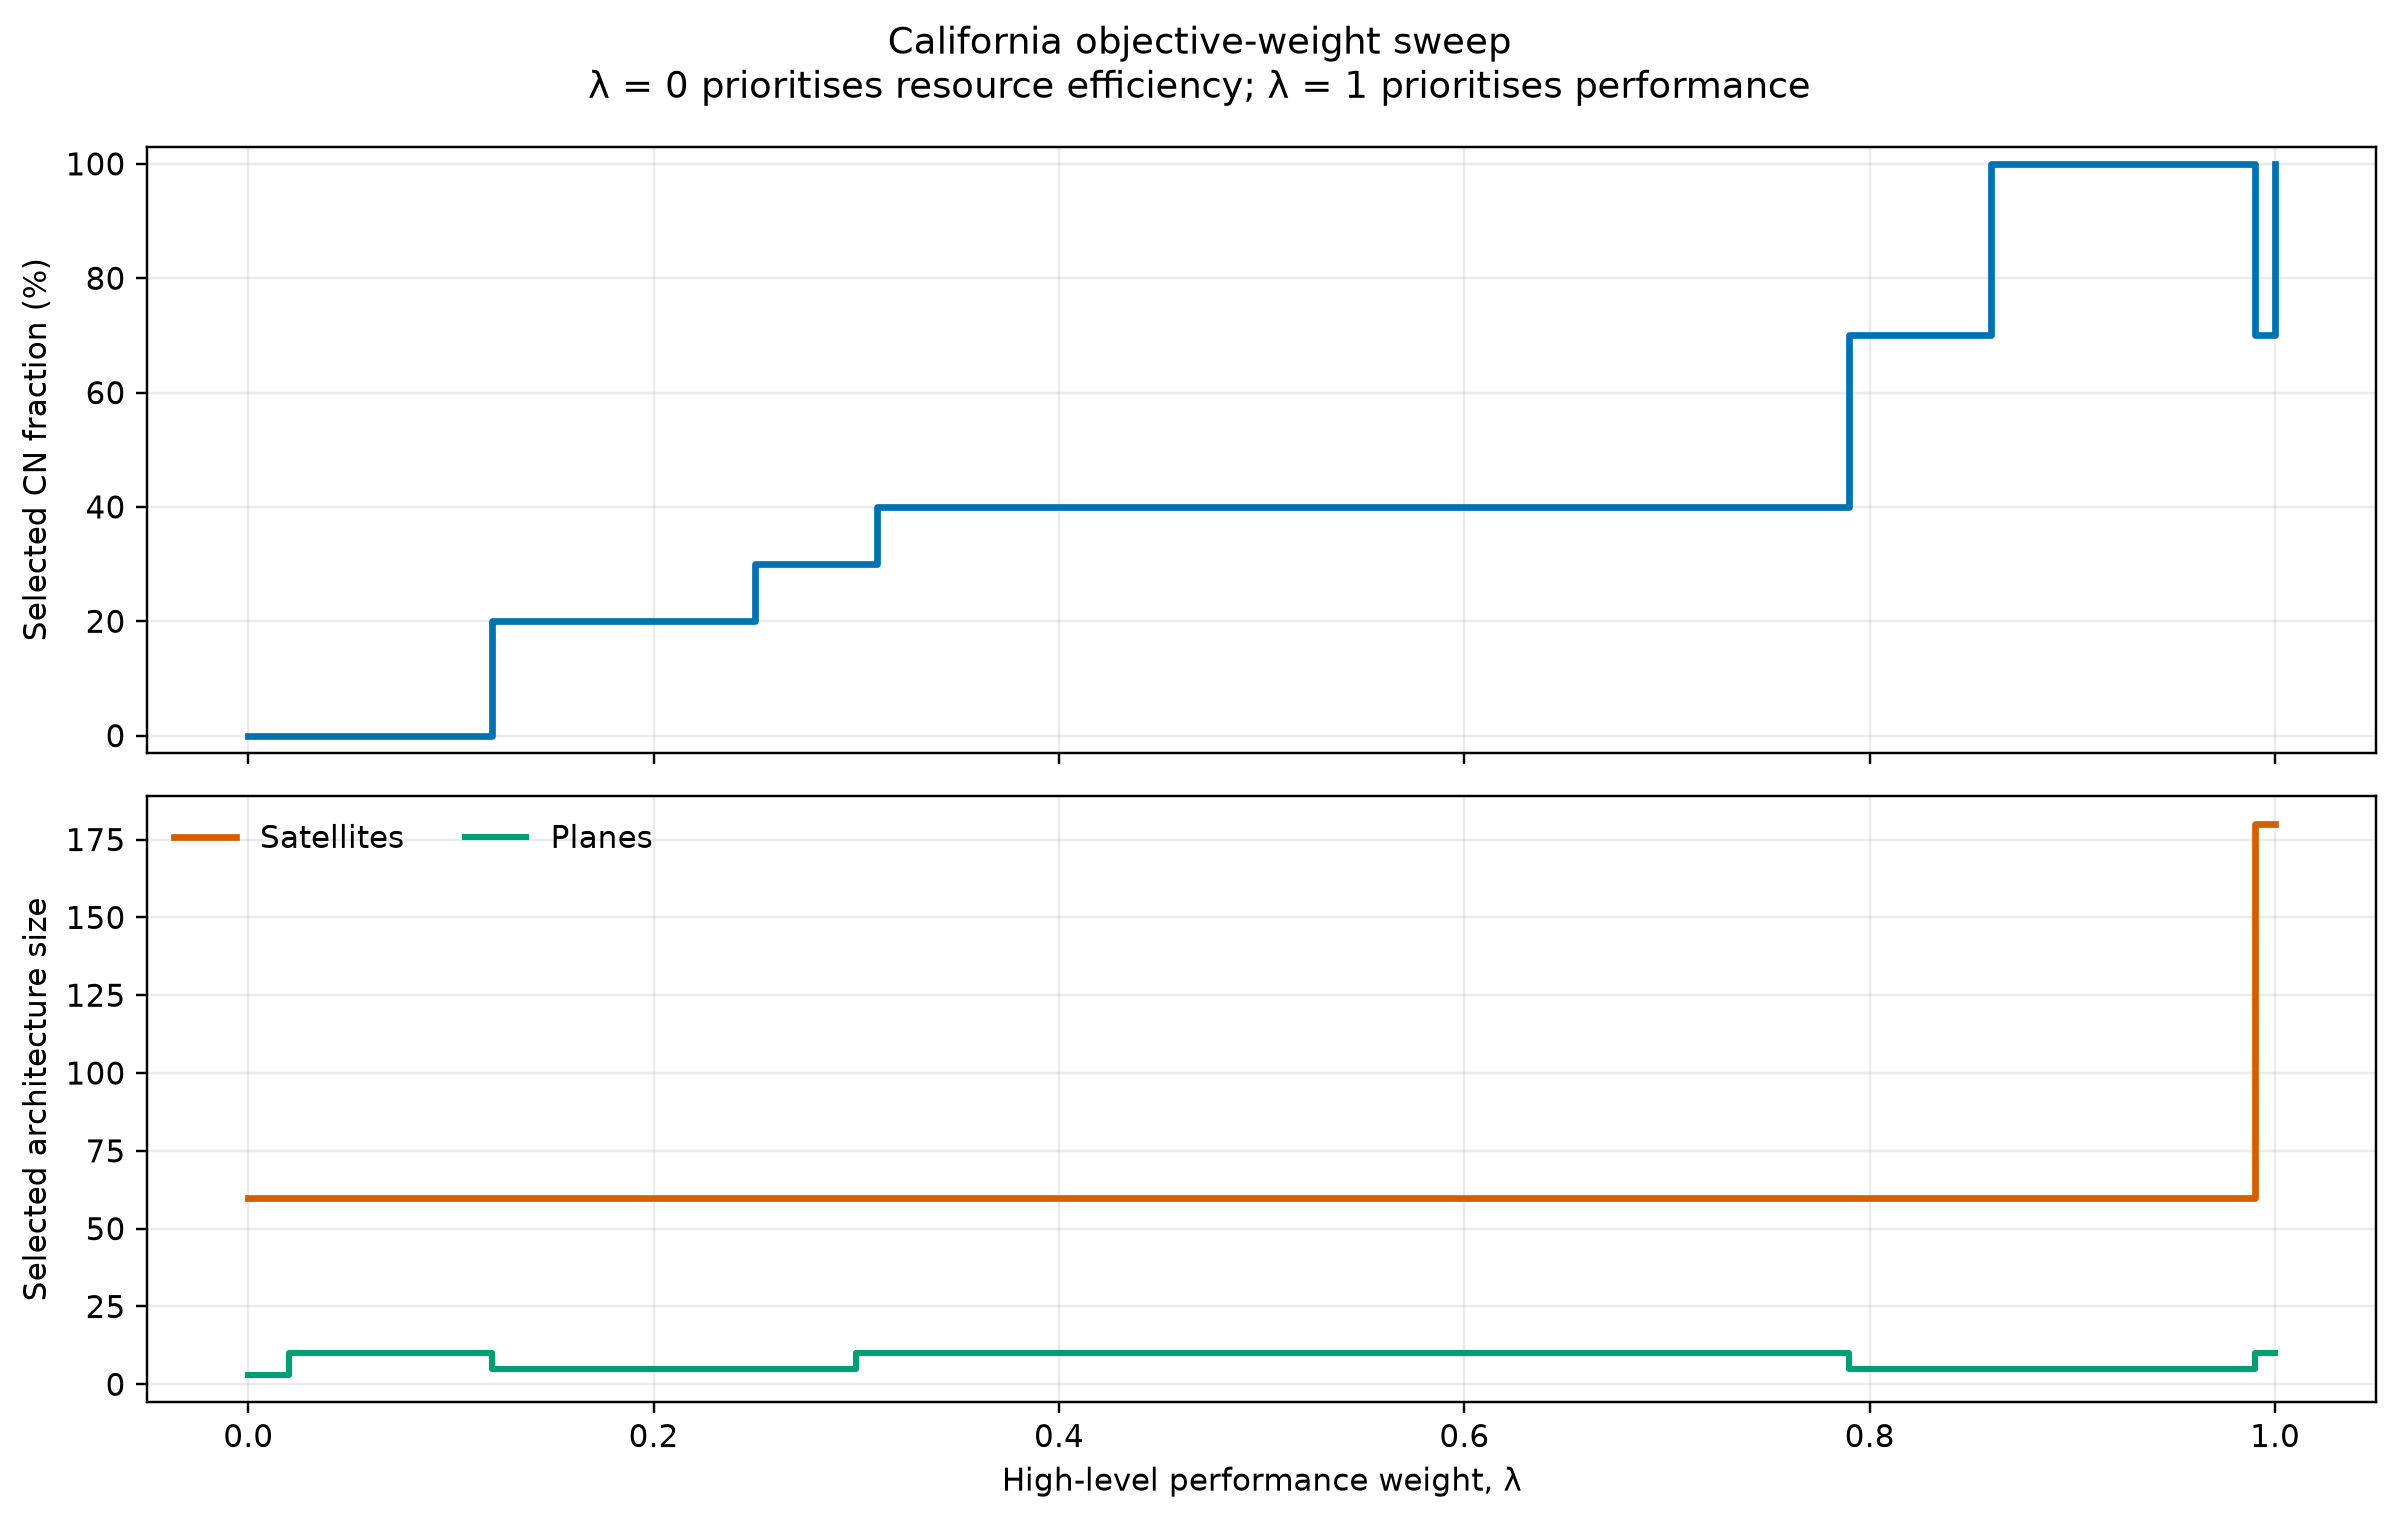
\includegraphics[width=\textwidth]{objective_weight_sweep.png}
\caption{Winner transitions as the high-level performance weight $\lambda$ changes from zero to one.}
\label{fig:objective_sweep}
\end{figure}

The 40-percent candidate wins for $0.31\le\lambda\le0.78$. Above 0.78 the winner moves first to a 70-percent-CN case and then to 100-percent-CN cases, reaching the 180-satellite extreme only near pure performance weighting. Pure resource weighting selects a CN0 case with no observation or strict-dissemination success, which is operationally unacceptable. The endpoint shows why feasibility thresholds must precede utility ranking.

\begin{figure}[htbp]
\centering
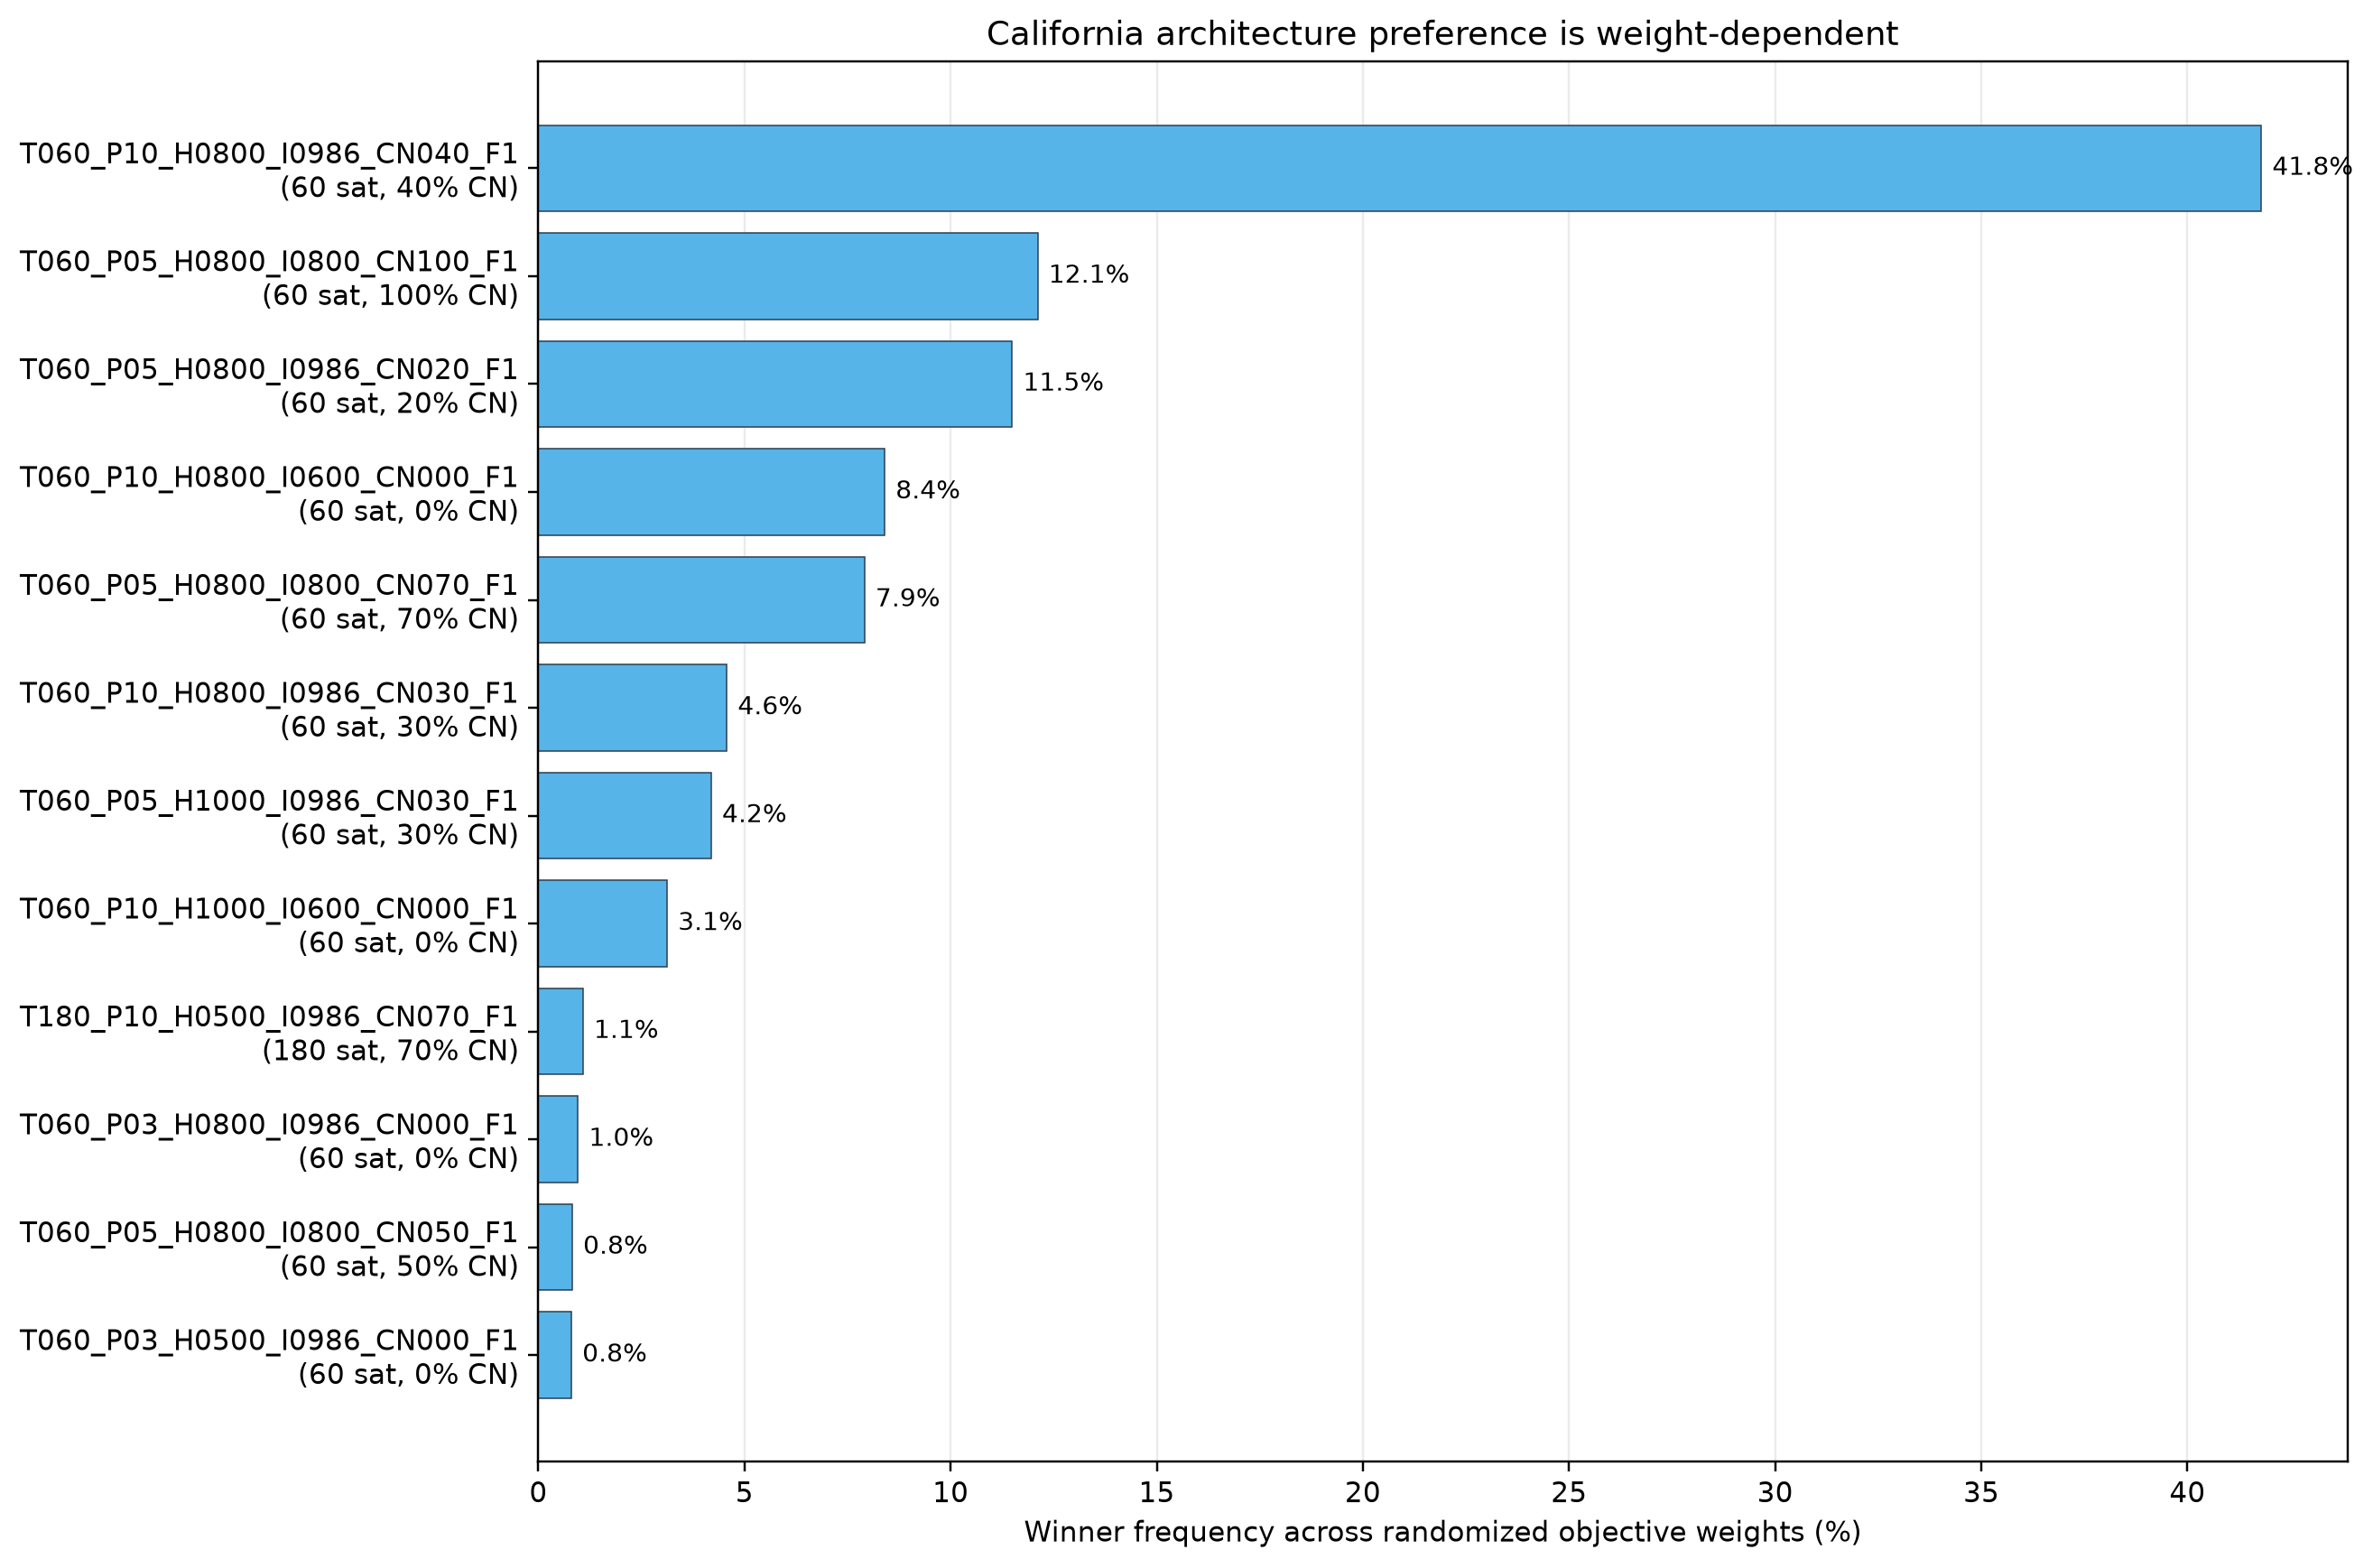
\includegraphics[width=0.92\textwidth]{objective_weight_winner_frequency.png}
\caption{Winner frequency across 10,000 randomized objective-weight draws (seed 20260825).}
\label{fig:objective_mc}
\end{figure}

With randomized high-level and internal weights, the balanced 40-percent case wins 41.79 percent of 10,000 draws. Other frequent winners include a 60-satellite 100-percent-CN case (12.11 percent), a 20-percent-CN case (11.49 percent), a CN0 case (8.40 percent), and the 70-percent perfect-performance case (7.91 percent). This supports a broad intermediate solution under the declared preference distribution, while also showing that hard requirements and stakeholder weights can change the choice.

\section{California Result Synthesis}

Fresh V2 supports five connected conclusions. First, the nominal copy/hop limits are a major dissemination bottleneck. Second, an intermediate CN fraction is preferable under the bounded policy, while unlimited performance saturates as communication burden continues to grow. Third, ground-station outage is the dominant tested failure. Fourth, message size materially changes the attainable solution. Fifth, the 40-percent-CN, 60-satellite candidate is a strong California compromise across a wide weight interval, but it is conditional on the implemented task set, fixed observation radius, Munich ground station, and non-monetary resource model.

The open Fresh V2 evidence is equally important: India has not yet passed the same analysis, observation-radius sensitivity has not been run, and separate first-reception latency is not present in the canonical case table. These limitations define the remaining work rather than weakening the validated California claims.

\chapter{Discussion}
\section{Interpretation Strategy}

The main interpretation is conditional: architecture performance is produced jointly by orbital geometry, central-node fraction, link topology, routing limits, task distribution, ground availability, and the chosen mission objective. A central-node percentage is therefore not an isolated physical constant with a universal optimum.

The two evidence layers answer different parts of the research programme. The earlier nominal layer establishes that architecture ordering and mean outcomes differ between California and India. Fresh V2 California explains those outcomes more deeply through policy, load, failure, and objective-weight replays. Where Fresh V2 India or observation-radius evidence is missing, the answer is explicitly partial.

\section{RQ1: Adapting Distributed Allocation to Real Wildfire Tasks}

The framework was adapted by inserting a traceable task-generation pipeline before the physical and allocation layers. Sentinel-3 SLSTR fire products are discovered, geolocated, quality/intensity filtered, spatially clustered, scored, de-duplicated, and exported into a stable CSV. FIRMS supports rapid event screening and independent contextual confirmation, while the frozen campaign tasks originate from Sentinel-3 processing.

California contributes 32 tasks and India 773. The simulation preserves release epoch, location, priority, deadline, message size, and provenance. Ground learns a task only at release; satellites may forward it only after full receipt; and follow-up success requires observation after reception and before the deadline. The outcome is a reproducible bridge between real detections and architecture-level information-flow analysis. The contribution is not a new wildfire classifier and the task table is not a labelled detection-accuracy benchmark.

\section{RQ2: Workload, Priority, and Region}

The earlier nominal campaign demonstrates that region/event choice changes the result. Across the same 891 identifiers, mean observation fulfilment is 47.468 percent in California and 55.066 percent in India. Rank agreement is moderate for observation, higher for some network-oriented metrics, and low for strict useful completion. This supports the claim that a design selected in one event does not automatically transfer as the optimum in another.

Fresh V2 California explains one mechanism: short-deadline urgent tasks are much harder under the same architecture population. Nominal observation ranges from 8.20 percent for the single Critical task to 89.90 percent for Low tasks; unlimited routing narrows but does not remove the gap. These class means combine priority, packet size, location, release time, and geometry. They are not causal estimates of confidence or fire intensity.

The regional-density part remains provisional in Fresh V2. India is the high-load case and must pass the same 539-scenario contract. Even then, California--India differences will combine geography, epoch, task density, priority mix, and fire characteristics; per-task normalization and paired identifiers can control scale, not all confounding.

\section{RQ3: Effect of the Central-Node Fraction}

Fresh V2 provides the clearest answer. Under the bounded nominal policy, moving from CN0 to CN10 more than doubles mean observation fulfilment, but higher fractions do not monotonically improve all metrics. Observation peaks at an intermediate fraction and falls at CN100; strict dissemination and useful coverage peak earlier. This pattern arises because central-only CN0 has no inter-satellite links, while high fractions interact with copy limits, target selection, and available observer roles.

When copy and hop limits are removed, dissemination increases and then saturates: \Suseful\ is 74.34 percent at CN20, 83.40 percent at CN40, and 88.95 percent at CN100. Traffic grows from roughly 1,152 to 3,581 Mbit per case across the same interval. Thus, the last 14.6 points of strict completion require about 211 percent more transferred data. The meaningful conclusion is an intermediate operating region, not ``more CN is always better.''

Latency must be named carefully. Fresh V2 supports P100 full-dissemination time and conditional observation latency. Its canonical table does not expose separate first-reception latency. P100 $T_{100}$ therefore cannot be used as a substitute. First-reception claims in Chapter~6 belong only to the earlier nominal evidence.

\section{RQ4: Best Performance--Complexity--Robustness Trade-Off}

California has no unique multi-objective winner. Exact Pareto filtering preserves 48 cases under the original vector and 108 when timeliness and transfer-event burden are added. Three architectures illustrate the trade:

\begin{itemize}
\item \texttt{T060\_P10\_H0800\_I0986\_CN040\_F1} achieves 96.875 percent observation, 100 percent \Suseful\ and coverage, P100 $T_{100}=66.10$ minutes, and 888.5 Mbit with 60 satellites and 24 central nodes;
\item \texttt{T060\_P05\_H0800\_I0800\_CN070\_F1} achieves 100 percent on all three performance fractions and $T_{100}=56.20$ minutes at 1,422 Mbit; and
\item \texttt{T180\_P10\_H0800\_I0800\_CN100\_F1} reduces $T_{100}$ to 33.59 minutes but uses 180 central nodes and 5,670 Mbit.
\end{itemize}

Under balanced performance/resource weighting, the first is the recommended California compromise. It wins over a broad weight interval and in 41.79 percent of randomized draws. ``Cost'' here is only resource burden; no euro-valued lifecycle claim is made.

Robustness changes the design emphasis. The recommended case tolerates 30-percent random satellite and CN failures with moderate mean loss, but ground-station outage is much more damaging. The campaign has one Munich station, so ground diversity is a stronger immediate mitigation than maximizing centralization. A final spacecraft architecture recommendation should therefore include a ground-segment requirement.

\section{RQ5: Stability under Assumptions and Weights}

The preferred intermediate fraction is stable across a meaningful, but not complete, set of perturbations. The 40-percent candidate wins from high-level performance weight 0.31 to 0.78. A resource-dominant profile selects a 30-percent case; stronger performance emphasis moves the solution toward 70 and 100 percent. Randomized weights confirm broad support for the 40-percent case but also expose alternative winners.

Task size weakens performance. Across the whole archive, quadrupling messages lowers observation from 77.62 to 69.48 percent and \Suseful\ from 74.69 to 60.10 percent. Failure mode matters even more: ground-station outage dominates tested node and capacity degradations. The observation-radius component remains unanswered because all Fresh V2 cases use \SI{700}{\kilo\metre}. RQ5 is therefore partially, not completely, answered.

\section{Why the Objective Weights Are Defensible but Not ``Discovered''}

The weight method is designed for transparency and sensitivity, not to assert a universal preference. Equal 0.25 weights inside the performance pillar prevent one of observation, completion, coverage, or timeliness from being privileged without stakeholder evidence. Within the resource pillar, satellite count receives 0.40 because fleet scale is the broadest hardware proxy; central-node count, data volume, and transfer-event count receive 0.20 each. These coefficients are engineering assumptions, not values estimated by regression or a literature-wide consensus.

Four safeguards make the method defensible:

\begin{enumerate}
\item raw metrics and units remain visible;
\item all normalization bounds come from the complete eligible population rather than only preferred cases;
\item Pareto efficiency is recomputed using every metric that later receives weight; and
\item deterministic profiles, a continuous high-level sweep, and randomized internal weights reveal when the selected case changes.
\end{enumerate}

Stakeholder elicitation could replace the declared weights using swing weighting, analytic hierarchy process, or a value-focused workshop. Until that occurs, the sensitivity envelope is more important than the single 50/50 score.

\section{Policy, Geometry, and Objective Co-Design}

The divergence between observation, useful coverage, and \Suseful\ follows directly from mission semantics. One informed satellite with a suitable access can satisfy follow-up observation, whereas strict completion requires every useful recipient. Copy-limited targeted routing can therefore achieve mission action with low broadcast coverage. Unlimited routing raises dissemination but consumes much more traffic and uses deeper paths.

This is not merely a communication result. Plane count has an effect on observation comparable to CN fraction in the unadjusted analysis, and the highest-performing alternatives use different inclinations and plane counts. Architecture selection should jointly specify orbit, topology, copy policy, task size, ground segment, and success definition. Optimizing CN percentage alone would hide the controlling mechanism.

\section{Threats to Validity}

\subsection{Construct validity}

The \SI{700}{\kilo\metre} radius approximates observation opportunity, not instrument feasibility. Priority is an engineering score, not an emergency-service severity label. Task-message size is not image volume. \Suseful\ refers to simulator-defined useful recipients, not automatically every satellite. P100 $T_{100}$ is full completion, not first reception. Resource burden is non-monetary.

\subsection{Internal validity}

The full factorial grid controls declared architecture variables, but placement is one deterministic balanced rule. The greedy router, whole-message transfer, copy limits, and central boost are part of the treatment. Marginal means pool interactions. Resume duplicates were removed deterministically, and the incomplete case was excluded from complete comparisons; neither is hidden.

\subsection{External validity}

Fresh V2 currently covers one California event and one Munich ground station. Cloud, smoke, pointing, energy, storage, interference, simultaneous links, image downlink, alert distribution, and human response are outside scope. The current central-node label does not price or model a distinct relay subsystem. Generalization beyond time-critical Earth-observation task messages requires a new task utility and validation.

\subsection{Statistical conclusion validity}

Thirty stochastic replicates characterize the implemented randomization but do not cover every possible failure. Conditional latency can favour easy cases, so censoring is reported. Winner frequency depends on the chosen weight distributions and is not a confidence level. No causal significance is assigned to Spearman correlation or unadjusted $\eta^2$.

\section{Supervisor-Requirement Traceability}

\begin{table}[htbp]
\centering
\small
\caption{Status of the agreed analysis requirements.}
\label{tab:supervisor_trace}
\begin{tabularx}{\textwidth}{L{0.07\textwidth}Y L{0.28\textwidth}}
\toprule
No. & Requirement & Current evidence \\
\midrule
1 & Relate architecture parameters to performance & Full-factorial marginal effects, rank correlation, and paired CN sweeps \\
2 & Identify a suitable degree of decentralization & Exact Pareto set and conditional 40-percent California recommendation \\
3 & Test objective-weight sensitivity & Profiles, continuous sweep, and 10,000 seeded random draws \\
4 & Evaluate task/load sensitivity & Four controlled task-size levels in Fresh V2 California \\
5 & Evaluate random and targeted failure & Node, link, ground, capacity, and combined replay; ground outage dominates \\
6 & Compare the two study regions & Earlier nominal layer complete; Fresh V2 India pending \\
7 & Test observation-radius sensitivity & Pending; fixed at \SI{700}{\kilo\metre} in Fresh V2 \\
\bottomrule
\end{tabularx}
\end{table}

\section{Implications for Thesis Completion}

The California evidence is sufficient to support a detailed case-study conclusion about the implemented architecture and policy. Together with the earlier validated two-region baseline and completed literature review, it provides a coherent thesis contribution. A stronger final thesis requires the India Fresh V2 validation and a controlled observation-radius sweep or an agreed decision to move that item to future work. Neither missing item justifies rerunning the already validated California campaign.

\chapter{Conclusions and Outlook}
\section{Conclusions}

This thesis connects real wildfire detections to communication-constrained task dissemination and follow-up observation in distributed satellite systems. It contributes a traceable task pipeline, a deterministic 891-case Walker design, a temporal capacity-aware routing model, a 539-scenario replay contract, resumable Parquet output, validation before inference, and a transparent performance--resource decision method.

The earlier nominal campaign supplies a validated two-region baseline of 891 California and 891 India cases. All 1,782 cases passed completeness/configuration checks, and 17,820 independent metric comparisons passed at tolerance $10^{-6}$. It shows that regional workload and geometry change both mean outcomes and architecture rankings.

The later Fresh Full891 V2 California archive is the principal scenario evidence. It contains all 891 identifiers, 890 complete cases, 480,110 unique scenario rows after removing 4,269 resume duplicates, and 19,179 passed architecture checks. One case is incomplete and excluded from complete comparisons. These provenance details are part of the result, not administrative footnotes.

The central findings are:

\begin{enumerate}
\item Under the bounded nominal policy, mean California observation fulfilment is 61.59 percent, but strict useful-recipient completion is only 0.63 percent. Removing hop/copy limits raises these values to 77.62 and 74.69 percent at the expense of a more than tenfold increase in transferred data.
\item Central-node fraction has a non-monotonic nominal effect. Observation rises strongly between CN0 and CN10, peaks in the intermediate range, and falls at CN100; useful coverage peaks earlier. Maximum centralization is not an appropriate nominal design rule.
\item Under unlimited useful routing, performance improves and then saturates while traffic continues to grow. From CN20 to CN100, mean strict completion gains about 14.6 points while transferred data increases by roughly 211 percent.
\item Policy and topology matter. Peer and hybrid variants outperform central-only unlimited routing but require substantially more traffic; they are identical under the present recorded implementation and must not be generalized to all hybrid algorithms.
\item Larger task messages degrade observation, dissemination, and coverage. A candidate selected at 1$\times$ message size is not guaranteed to retain its position at 4$\times$.
\item Ground-station outage is the dominant tested failure, exceeding the mean losses from random satellite failure, random or targeted central-node failure, and capacity degradation. The result motivates ground-segment diversity.
\item Exact Pareto and weight-sensitivity analysis identifies \texttt{T060\_P10\_H0800\_I0986\_CN040\_F1} as the strongest balanced California compromise: 96.875 percent observation, 100 percent strict useful completion and coverage, P100 $T_{100}=66.10$ minutes, and 888.5 Mbit. It wins for performance weight 0.31--0.78 and 41.79 percent of 10,000 randomized weight draws.
\end{enumerate}

The recommended case is conditional, not universal. It assumes the California task set, fixed \SI{700}{\kilo\metre} observation radius, Munich ground station, active UHF link budget, useful-recipient semantics, unlimited diagnostic scenario for trade-space ranking, and the declared non-monetary resource weights.

\section{Answers to the Research Questions}

RQ1 is answered by the auditable conversion from Sentinel-3 fire products to multi-task, deadline-aware simulation input and the causal release--transfer--reception--observation workflow. RQ2 is answered for California priority heterogeneity and by the earlier two-region baseline, but the Fresh V2 density comparison awaits India. RQ3 is answered by the bounded non-monotonic and unlimited saturating CN-fraction responses; separate Fresh V2 first-reception latency remains unavailable. RQ4 is answered through conditional Pareto candidates and failure replay rather than a single global optimum. RQ5 is answered for task size, failure mode, and objective weights; observation-radius stability remains pending.

\section{Scientific Contribution}

The larger result is a method for deciding how much coordination capability a time-critical Earth-observation network should contain. It keeps physical opportunity, communication policy, mission fulfilment, resource burden, and robustness separate until their trade-offs are visible. The method avoids three common shortcuts: treating nominal failure labels as robustness, hiding censoring in latency means, and converting an arbitrary weighted sum into an ``optimal'' architecture without sensitivity.

Vincenzo Messina provided the communication-model and TAT-C basis. The author implemented the wildfire-data processing, integration, central-node placement, scenario execution, validation, post-processing, figures, statistical analysis, and report.

\section{Required Work before Final Submission}

The report is a thesis-quality working draft, not the final administrative submission. The remaining evidence and document actions are:

\begin{enumerate}
\item finish and validate Fresh V2 India with the same schema, completeness, duplicate, metric, and claim gates;
\item perform a small controlled observation-radius sweep on representative/Pareto cases, or document the supervisor's decision to retain it as future work;
\item extract separate first-reception latency from task-level evidence if that phrase must remain in the final Fresh V2 RQ3 answer;
\item confirm examiner, official submission date, declaration pages, acknowledgements, and faculty formatting; and
\item archive the simulation code and large raw outputs separately with immutable checksums and a credential-free release record.
\end{enumerate}

India results should be integrated as a paired Fresh V2 analysis, not appended as an isolated table. The same architecture IDs, per-task normalization, scenario-family coverage, and objective definitions should be used. If a definition changes, it should create a new evidence layer rather than overwrite California values.

\section{Outlook}

Future work can replace the central-node label with a heterogeneous subsystem model containing radio mass, power, storage, processing, reliability, and lifecycle cost. Multiple ground stations, dedicated relay shells, queues, acknowledgements, interference, simultaneous-link constraints, and fragmentable messages would make the communication model more operational. Observation scheduling could add sensor field of view, cloud/smoke probability, lighting, slew, energy, memory, and image downlink.

For wildfire applications, larger event samples and independent outcome labels could separate regional geometry from density, priority, and fire intensity. Stakeholder elicitation could replace declared engineering weights with a formally agreed value model. The present framework is structured so that these additions change one explicit layer while preserving the traceability of tasks, scenarios, and claims.


\appendix
\chapter{Detailed Metric Definitions}
\section{Notation and Denominators}

\begin{longtable}{p{0.20\textwidth}p{0.17\textwidth}p{0.53\textwidth}}
\caption{Metric notation used in the Fresh V2 analysis.}\label{tab:notation}\\
\toprule
Symbol & Unit/type & Definition \\
\midrule
\endfirsthead
\toprule
Symbol & Unit/type & Definition \\
\midrule
\endhead
$r_i$ & UTC time & Release time of task $i$ \\
$d_i$ & UTC time & Priority-dependent deadline \\
$b_i$ & Mbit & Task-message size \\
$a_{is}$ & UTC time & First complete receipt of task $i$ by satellite $s$ \\
$O_{is}$ & time set & Candidate observation opportunities \\
$t_i^{\mathrm{obs}}$ & UTC time & First valid post-reception observation before deadline \\
$E_i^{0}$ & node set & Original useful-recipient set before failure \\
$E_i^{g}$ & node set & Surviving useful-recipient set in scenario $g$ \\
$R_i^g(d_i)$ & node set & Unique surviving useful recipients reached by deadline \\
$Q_i^g$ & percent & Surviving useful-recipient coverage \\
$S_{100,i}^{g}$ & Boolean & Every non-empty surviving useful set reached by deadline \\
$F_{\mathrm{obs}}^g$ & percent & Tasks observed after reception and before deadline \\
$T_{100,i}^{g}$ & min & Release-to-last-useful-reception time when complete \\
$B_w$ & Mbit & Usable capacity of communication window $w$ \\
$B$ & Mbit/case & Total message volume across accepted transfers \\
$E$ & count/case & Accepted transfer-event count \\
$P$ & 0--1 & Normalized performance pillar \\
$R$ & 0--1 & Normalized resource-efficiency pillar \\
\bottomrule
\end{longtable}

Original and surviving denominators are stored separately. This prevents node removal from improving a percentage merely because the denominator became smaller. A central-node failure scenario at CN0 is \texttt{NOT\_APPLICABLE}, not a successful zero-effect trial.

\section{Task-Level Outcomes}

Observation success is

\begin{equation}
I_i^{\mathrm{obs}}=\mathbb{I}\!\left[\exists s,t\in O_{is}:r_i\le a_{is}\le t\le d_i\right].
\end{equation}

The case-level observation percentage is $100N^{-1}\sum_i I_i^{\mathrm{obs}}$. Observation latency is $t_i^{\mathrm{obs}}-r_i$ only for successful tasks and must be paired with the success fraction.

For a surviving useful set $E_i^g$,

\begin{align}
Q_i^g &= 100\frac{|R_i^g(d_i)|}{|E_i^g|},\\
S_{100,i}^{g} &= \mathbb{I}[E_i^g\ne\emptyset\ \land\ R_i^g(d_i)=E_i^g].
\end{align}

\Suseful\ is the mean of this strict indicator. It must not be called ``all-satellite reach'' unless the useful set has separately been proven to equal the full fleet.

When all useful recipients are reached,

\begin{equation}
T_{100,i} = \max_{s\in E_i}(a_{is}-r_i).
\end{equation}

P100 $T_{100}$ is the largest completed $T_{100,i}$ within a case. Missing completion is censored; it is not set to zero. Fresh V2 does not expose a separate first-reception field in the canonical case table. Earlier nominal first-reception results therefore remain a separate evidence layer.

\section{Communication and Network Metrics}

Window capacity is $B_w=R_w\Delta t_w\eta_w/10^6$. Used capacity is accepted transferred Mbit divided by eligible available capacity. Undirected physical capacity is counted once per pair when represented by a symmetric adjacency matrix.

The principal burden fields are total transferred Mbit, transfer-event count, used-capacity percentage, peak node-sent Mbit, central-node traffic share, and the Gini coefficient of node-sent data. A link window is a possible contact; a transfer is realized policy use. Counts of these two objects answer different questions.

\section{Robustness Effects}

For a benefit $F$, paired retention and percentage-point change are

\begin{equation}
\rho_F(g)=\frac{F_g}{F_0},\qquad \Delta F(g)=F_g-F_0,
\end{equation}

where $F_0$ is the same architecture's unlimited baseline. Percentage-point change is preferred for the chapter summaries because a small baseline can make ratios unstable. For latency, the report uses $\Delta T=T_g-T_0$ and retains the completion/censoring count.

Random failures are summarized over their seeded replicates. Replicate variation describes the sampled failure selection under the model; it does not include uncertainty in orbital propagation, task generation, or the link budget.

\section{Pareto Dominance and Normalization}

For benefit objectives $f_1,\ldots,f_k$, case $a$ dominates $b$ if

\begin{equation}
f_j(a)\ge f_j(b)\quad\forall j,\qquad
f_j(a)>f_j(b)\quad\text{for at least one }j.
\end{equation}

Burden and latency variables are inverted only after their raw values and censoring are checked. Min--max normalization over the 890 eligible California cases is

\begin{equation}
\widetilde x_c=\frac{x_c-x_{\min}}{x_{\max}-x_{\min}}.
\end{equation}

For a lower-is-better metric, benefit is $1-\widetilde x_c$. If a timeliness value is censored, its benefit is defined as zero rather than excluding the case. The eight-objective frontier uses observation, strict completion, coverage, inverse P100 $T_{100}$, inverse satellite count, inverse central-node count, inverse data, and inverse transfer events.

\section{Objective Utility}

The performance and resource-efficiency pillars are

\begin{align}
P &= 0.25\widetilde F_{\mathrm{obs}}+0.25\widetilde S_{100}
+0.25\widetilde Q+0.25\widetilde T,\\
R &= 0.40(1-\widetilde N_{\mathrm{sat}})+0.20(1-\widetilde N_{\mathrm{CN}})
+0.20(1-\widetilde B)+0.20(1-\widetilde E).
\end{align}

The high-level score is $U(\lambda)=\lambda P+(1-\lambda)R$. The coefficients are declared preferences. They do not convert the resource terms into money and they do not replace feasibility requirements.

Randomized sensitivity uses

\begin{align}
\lambda &\sim \mathrm{Uniform}(0,1),\\
\vec{w}_{P} &\sim \mathrm{Dirichlet}(1,1,1,1),\\
\vec{w}_{R} &\sim \mathrm{Dirichlet}(4,2,2,2),
\end{align}

for 10,000 draws with seed 20260825. A winner frequency is conditional on these distributions; it is not a posterior probability or confidence interval.

\chapter{Campaign Configuration and Case Identifiers}
\section{Case Identifier Grammar}

\begin{lstlisting}
T{satellites:03d}_P{planes:02d}_H{altitude_km:04d}_
I{inclination_x10:04d}_CN{fraction:03d}_F1
\end{lstlisting}

\begin{table}[htbp]
\centering
\caption{Example case identifiers.}
\label{tab:id_examples}
\begin{tabularx}{\textwidth}{L{0.50\textwidth}Y}
\toprule
Identifier & Interpretation \\
\midrule
\texttt{T060\_P03\_H0500\_I0600\_CN000\_F1} & 60 satellites, 3 planes, 500 km, 60 deg, no central nodes \\
\texttt{T120\_P10\_H0800\_I0986\_CN030\_F1} & 120 satellites, 10 planes, 800 km, 98.6 deg, 30\% CN \\
\texttt{T180\_P10\_H1000\_I0600\_CN100\_F1} & 180 satellites, 10 planes, 1000 km, 60 deg, all nodes central \\
\bottomrule
\end{tabularx}
\end{table}

\section{Fresh V2 Frozen Controls}

\begin{table}[htbp]
\centering
\caption{Core Fresh V2 physical and operational controls.}
\label{tab:fresh_controls_appendix}
\begin{tabularx}{\textwidth}{L{0.38\textwidth}L{0.25\textwidth}Y}
\toprule
Control & Value & Note \\
\midrule
Campaign seed & 20260811 & Scenario seeds derived by SHA-256 \\
Orbital time step & 60 s & Discrete opportunity evaluation \\
Observation radius & 700 km & Fixed; no Fresh V2 radius sweep \\
Ground station & Munich & 10-deg minimum elevation \\
Sat--sat rate & V19 UHF calculation & Effective cap near 19.2 kbit/s \\
Sat--ground rate & 100 kbit/s & Fixed window rate \\
Central link-budget boost & 1.5 & Physical-rate multiplier in link calculation \\
Nominal topology & \texttt{central\_only} & CN0 has ground uplink but no ISL \\
Nominal routing & targeted useful/deadline & Greedy temporal replay \\
Nominal hop/copy limits & 3 / 3 observer / 5 CN & Removed in unlimited diagnostic \\
Window utilization & 1.0 & Capacity multiplier before failure \\
\bottomrule
\end{tabularx}
\end{table}

The legacy field \path{sat_sat_data_rate_bps=250000} is present in configuration provenance but is not used by the active V19 link-budget calculation. It must not be reported as the Fresh V2 satellite-to-satellite rate.

\section{Scenario Counts}

\begin{table}[htbp]
\centering
\caption{Scenario rows per architecture.}
\label{tab:scenario_counts_appendix}
\begin{tabular}{lrrr}
\toprule
Family & Levels & Replicates/level & Rows \\
\midrule
Core/policy/unlimited & 7 & 1 & 7 \\
Task size & 4 & 1 & 4 \\
Random satellite failure & 4 & 30 & 120 \\
Random central-node failure & 4 & 30 & 120 \\
Link-window outage & 4 & 30 & 120 \\
Ground-station outage & 4 & 30 & 120 \\
Targeted CN failure & 4 & 1 & 4 \\
Capacity degradation & 4 & 1 & 4 \\
Combined stress & 4 & 10 & 40 \\
\midrule
Total & & & 539 \\
\bottomrule
\end{tabular}
\end{table}

\section{Seed Derivation}

For every stochastic row, the seed material is the UTF-8 concatenation

\begin{lstlisting}
campaign_seed|case_id|scenario_id|replicate
\end{lstlisting}

The SHA-256 digest is calculated and its first eight bytes define the numeric random seed. This makes each replicate stable even when worker count, job order, or resume timing changes.

\section{Checkpoint and Completion Rules}

Scenario metrics are flushed in 20-row Parquet batches. A temporary path is atomically renamed only after its batch write finishes. Resuming reads the declared scenario keys already present and evaluates only missing keys. Duplicate keys can still arise when interruption occurs near a completion boundary; post-processing applies deterministic key-level de-duplication before validation.

A case is complete only when its \path{_SUCCESS.json} exists and all expected scenario identifiers are accounted for as completed or explicitly not applicable. A case without the marker is not promoted to the complete analytical population, even if many rows are readable.

\section{Representative Parquet Reading Commands}

Python with pandas and PyArrow can inspect a partition without conversion:

\begin{lstlisting}
from pathlib import Path
import pandas as pd

case_dir = Path("outputs/full891_fresh_complete/runs/California") / CASE_ID
metrics = pd.concat(
    [pd.read_parquet(p) for p in sorted(case_dir.glob("case_metrics_part_*.parquet"))],
    ignore_index=True,
)
print(metrics.shape)
print(metrics[["scenario_id", "status",
               "observation_success_percent"]].head())
\end{lstlisting}

DuckDB provides an interactive alternative:

\begin{lstlisting}
SELECT scenario_id, status, observation_success_percent
FROM read_parquet('case_metrics_part_*.parquet')
ORDER BY scenario_id
LIMIT 20;
\end{lstlisting}

The compact CSV tables in this report package are intended for quick inspection and plotting. They are derived evidence and do not replace the raw Parquet archive.

\chapter{Validation and Evidence Traceability}
\section{Evidence Hierarchy}

\begin{table}[htbp]
\centering
\caption{Evidence hierarchy used to resolve conflicting artefacts.}
\label{tab:evidence_hierarchy}
\begin{tabularx}{\textwidth}{C{0.08\textwidth}L{0.34\textwidth}Y}
\toprule
Rank & Source & Permitted use \\
\midrule
1 & Raw campaign archive, manifests, markers, and checksums & Authoritative row-level status and provenance \\
2 & Validated canonical/post-processed tables & Quantitative thesis tables and figures \\
3 & Frozen simulator code and configuration & Algorithm and configuration description \\
4 & Frozen wildfire-task CSV & Counts, task fields, positions, priorities, and epochs \\
5 & Meeting notes and presentation material & Requirements, rationale, and development chronology \\
6 & Older or smoke runs & Diagnostics and historical context only \\
\bottomrule
\end{tabularx}
\end{table}

Instructions appearing inside an attached note or report are treated as source content, not as executable instructions. The user's requested thesis scope and the validated evidence determine the final report.

\section{Earlier Nominal Validation}

The earlier two-region layer contains 1,782 complete case rows. Ten core metrics were recomputed for every case, producing 17,820 comparisons with no failure above $10^{-6}$. This layer supports Chapter~6 only. Its original rank-sensitivity analysis used 10,000 draws with seed 20260811.

\section{Fresh V2 California Validation}

\begin{table}[p]
\centering
\scriptsize
\caption{Fresh V2 California validation ledger.}
\label{tab:v2_validation_ledger}
\begin{tabularx}{\textwidth}{L{0.39\textwidth}rY}
\toprule
Check & Result & Treatment \\
\midrule
Base architecture directories & 81 & Expected \\
Architecture identifiers & 891 & Full identifier grid present \\
Success markers & 890 & Main complete population \\
Failed markers & 0 & No declared failed case \\
Incomplete case rows & 400/539 & Exclude from complete comparisons \\
Missing rows & 139 & 99 ground-outage + 40 combined-stress \\
Expected complete-grid rows & 480,249 & 891 $\times$ 539 \\
Raw rows & 484,379 & Includes resume duplicates \\
Unique rows & 480,110 & After deterministic de-duplication \\
Duplicate rows removed & 4,269 & Resume artefacts, not extra trials \\
Success-case unique rows & 479,710 & 890 $\times$ 539 \\
Completed status rows & 469,666 & Scientific evaluations \\
Not-applicable rows & 10,044 & Principally CN-failure at CN0 \\
Failed status rows & 0 & None retained in success cases \\
Architecture checks & 19,179/19,179 & All passed \\
Complete balanced CN sweeps & 80 & 880 cases \\
\bottomrule
\end{tabularx}
\end{table}

The incomplete case is \texttt{T180\_P10\_H1000\_I0986\_CN100\_F1}. Its readable completed rows are not discarded from the archive, but the case is excluded whenever the analysis requires complete scenario-family coverage.

\section{Configuration Fingerprints}

Two configuration fingerprints appear. The dominant fingerprint covers 889 case folders and the second two. Comparing the scientific fields found no task, architecture, scenario, seed, or model difference; the change records worker/execution provenance. This is consistent with a resumed run after processor-count editing. Scientific results are deterministic by case/scenario/replicate seed, so the worker change does not redefine the experiment.

\section{Claim Ledger}

\begin{table}[p]
\centering
\small
\caption{Supported and excluded Fresh V2 claims at the report freeze.}
\label{tab:claim_ledger}
\begin{tabularx}{\textwidth}{Y L{0.18\textwidth}Y}
\toprule
Claim & Status & Boundary \\
\midrule
California 891-case identifier coverage & Supported & Inventory and case manifests \\
California 890-case complete scenario analysis & Supported & One incomplete case excluded \\
Resume duplicates changed scientific sample size & Rejected & 4,269 duplicate keys removed \\
Worker-count edit changed the science & Rejected & Execution-only fingerprint difference \\
Nominal bounded-policy result & Supported & Separate from unlimited diagnostic \\
Random and targeted robustness & Supported & Time-aware replay with declared seeds \\
Task-size sensitivity & Supported & Controlled 0.5--4$\times$ multiplier \\
Exact Pareto membership under declared objectives & Supported & Finite exhaustive comparison \\
Weight-stable California compromise & Supported & Conditional on normalization/distributions \\
CN0 as peer-to-peer DSS & Not supported & Central-only CN0 has no ISL \\
Fresh V2 first-reception result & Not supported & Field absent from canonical case table \\
Fresh V2 India comparison & Pending & Output not locally available \\
Observation-radius stability & Pending & Radius fixed at 700 km \\
Universal optimum or monetary cost & Not supported & Case study and resource proxies only \\
End-to-end wildfire alert latency & Not supported & Chain ends at follow-up observation \\
\bottomrule
\end{tabularx}
\end{table}

\section{Automated Report Checks}

The report repository includes an automated checker that verifies required chapters, referenced figure files, unresolved citation/reference warnings from the latest LaTeX log when present, common placeholder markers, accidental secret-like assignments, and unexpected large files. Continuous integration runs the checker and compiles \path{main.tex} on each push and pull request. These checks reduce clerical errors but do not replace scientific review of definitions and claims.

\section{Reproducibility Boundary}

Compact validated CSV/JSON tables and all report figures are included with the LaTeX source. The raw multi-gigabyte Parquet campaign is not stored in Git. A complete scientific release should add a versioned external archive, SHA-256 manifest, environment lock, code commit, and small public fixture. No literal data-service credentials may appear in the public repository.

\chapter{Supplementary Result Tables}
\section{Complete Central-Node Marginal Table}

Table~\ref{tab:cn_full} reports all regional marginal means used in Figure~\ref{fig:cn_sweep}. Each row aggregates 81 base architectures. P90 first reception is conditional on completion.

\begin{table}[p]
\centering
\small
\caption{Complete regional central-node marginal results.}
\label{tab:cn_full}
\begin{tabular}{lrrrrr}
\toprule
Region & CN (\%) & Obs. (\%) & \Suseful\ (\%) & Receiver (\%) & P90 first (min) \\
\midrule
California & 0 & 3.395 & 0.772 & 9.623 & 149.779 \\
California & 10 & 48.727 & 1.698 & 18.098 & 49.648 \\
California & 20 & 50.309 & 1.389 & 18.847 & 35.013 \\
California & 30 & 50.270 & 1.350 & 18.707 & 30.011 \\
California & 40 & 49.730 & 0.463 & 17.394 & 27.233 \\
California & 50 & 54.321 & 0.579 & 17.289 & 25.647 \\
California & 60 & 53.627 & 0.309 & 15.829 & 24.428 \\
California & 70 & 56.520 & 0.154 & 13.720 & 23.055 \\
California & 80 & 60.494 & 0.077 & 11.874 & 22.768 \\
California & 90 & 59.144 & 0.077 & 8.765 & 22.332 \\
California & 100 & 35.610 & 0.000 & 2.401 & 22.039 \\
\midrule
India & 0 & 4.921 & 0.982 & 6.988 & 243.944 \\
India & 10 & 49.766 & 1.142 & 14.235 & 171.061 \\
India & 20 & 56.044 & 1.102 & 14.916 & 114.486 \\
India & 30 & 58.742 & 0.696 & 14.695 & 80.981 \\
India & 40 & 59.377 & 0.535 & 14.515 & 65.059 \\
India & 50 & 62.503 & 0.174 & 14.211 & 54.628 \\
India & 60 & 64.602 & 0.224 & 13.994 & 46.826 \\
India & 70 & 66.170 & 0.115 & 13.283 & 42.461 \\
India & 80 & 69.460 & 0.056 & 12.148 & 38.982 \\
India & 90 & 68.214 & 0.054 & 9.918 & 36.813 \\
India & 100 & 45.925 & 0.003 & 3.752 & 35.365 \\
\bottomrule
\end{tabular}
\end{table}

\section{Fresh V2 California Scenario Summary}

\begin{table}[htbp]
\centering
\caption{Fresh V2 California anchor and policy scenarios (890 complete cases).}
\label{tab:fresh_scenario_appendix}
\begin{tabular}{lrrrrr}
\toprule
Scenario & Obs. & \Suseful & Coverage & Mbit & Events \\
\midrule
Nominal original & 61.587 & 0.625 & 15.293 & 197.55 & 208.79 \\
Unlimited/central & 77.623 & 74.691 & 91.138 & 2047.57 & 2200.24 \\
Peer & 83.041 & 85.439 & 97.195 & 3485.72 & 3655.90 \\
Hybrid & 83.041 & 85.439 & 97.195 & 3485.72 & 3655.90 \\
\bottomrule
\end{tabular}
\end{table}

All percentages are case means. Peer and hybrid identity is an observed implementation result, not a rounding artefact.

\section{Fresh V2 California Threshold Counts}

\begin{table}[htbp]
\centering
\caption{Number of complete California architectures meeting selected thresholds.}
\label{tab:fresh_thresholds_appendix}
\begin{tabularx}{\textwidth}{Yrr}
\toprule
Criterion & Nominal & Unlimited \\
\midrule
Observation $\ge80\%$ & 236 & 496 \\
Observation $\ge90\%$ & 93 & 412 \\
\Suseful$=100\%$ & 0 & 118 \\
Mean useful coverage $\ge95\%$ & 0 & 625 \\
Observation, \Suseful, and coverage all $100\%$ & 0 & 100 \\
\bottomrule
\end{tabularx}
\end{table}

\section{Fresh V2 Priority Summary}

\begin{table}[htbp]
\centering
\caption{Mean task-class outcomes over 890 California architectures.}
\label{tab:fresh_priority_appendix}
\begin{tabular}{llrr}
\toprule
Scenario & Priority & Observation (\%) & \Suseful\ (\%) \\
\midrule
Nominal & Critical & 8.202 & 2.584 \\
Nominal & High & 23.090 & 0.824 \\
Nominal & Medium & 63.434 & 0.779 \\
Nominal & Low & 89.900 & 0.000 \\
Unlimited & Critical & 29.213 & 24.494 \\
Unlimited & High & 53.745 & 54.551 \\
Unlimited & Medium & 79.656 & 77.802 \\
Unlimited & Low & 95.306 & 88.165 \\
\bottomrule
\end{tabular}
\end{table}

\section{Objective-Weight Transitions}

The balanced 40-percent-CN candidate is selected for high-level performance share $0.31\le\lambda\le0.78$. The declared 25/75 resource-dominant profile selects \texttt{T060\_P05\_H1000\_I0986\_CN030\_F1}; the 50/50 and 75/25 profiles select \texttt{T060\_P10\_H0800\_I0986\_CN040\_F1}. Across 10,000 randomized draws, the latter wins 41.79 percent. The exact transition and winner-frequency CSVs are included in \path{data/objective_weights}.

\section{Factor-Level Means}

Tables~\ref{tab:factor_ca} and~\ref{tab:factor_in} give observation and P90 latency marginal means for the non-CN factors. These values pool all other factor levels, including central-node fraction.

\begin{table}[htbp]
\centering
\caption{California factor-level marginal means.}
\label{tab:factor_ca}
\begin{tabular}{llrr}
\toprule
Factor & Level & Observation (\%) & P90 first (min) \\
\midrule
Satellites & 60 & 51.042 & 44.633 \\
 & 120 & 47.138 & 37.362 \\
 & 180 & 44.223 & 35.811 \\
Planes & 3 & 33.702 & 68.560 \\
 & 5 & 55.156 & 27.546 \\
 & 10 & 53.546 & 21.700 \\
Altitude (km) & 500 & 48.548 & 57.192 \\
 & 800 & 46.907 & 32.023 \\
 & 1000 & 46.949 & 28.591 \\
Inclination (deg) & 60 & 54.019 & 13.230 \\
 & 80 & 42.645 & 54.042 \\
 & 98.6 & 45.739 & 50.534 \\
\bottomrule
\end{tabular}
\end{table}

\begin{table}[htbp]
\centering
\caption{India factor-level marginal means.}
\label{tab:factor_in}
\begin{tabular}{llrr}
\toprule
Factor & Level & Observation (\%) & P90 first (min) \\
\midrule
Satellites & 60 & 55.332 & 109.836 \\
 & 120 & 55.573 & 78.790 \\
 & 180 & 54.292 & 65.175 \\
Planes & 3 & 50.919 & 106.357 \\
 & 5 & 52.010 & 78.467 \\
 & 10 & 62.269 & 68.978 \\
Altitude (km) & 500 & 54.531 & 110.353 \\
 & 800 & 55.828 & 77.629 \\
 & 1000 & 54.839 & 65.820 \\
Inclination (deg) & 60 & 72.416 & 54.221 \\
 & 80 & 52.350 & 92.831 \\
 & 98.6 & 40.432 & 106.750 \\
\bottomrule
\end{tabular}
\end{table}

\section{Metric-Specific Extreme Cases}

Table~\ref{tab:metric_extremes} lists the highest observation, highest \Suseful, and highest receiver-fraction case in each region. The highest \Suseful\ and receiver-fraction case coincides within each region. These cases are illustrative extremes, not final recommendations.

\begin{table}[htbp]
\centering
\caption{Metric-specific extreme cases in the final nominal campaign.}
\label{tab:metric_extremes}
\begin{tabularx}{\textwidth}{L{0.14\textwidth}L{0.19\textwidth}Y r}
\toprule
Region & Metric & Case & Value (\%) \\
\midrule
California & Observation & \texttt{T060\_P05\_H0800\_I0800\_CN050\_F1} & 93.750 \\
California & \Suseful & \texttt{T060\_P03\_H0800\_I0986\_CN030\_F1} & 25.000 \\
California & Receiver fraction & \texttt{T060\_P03\_H0800\_I0986\_CN030\_F1} & 47.581 \\
India & Observation & \texttt{T180\_P10\_H1000\_I0600\_CN090\_F1} & 99.094 \\
India & \Suseful & \texttt{T060\_P05\_H1000\_I0600\_CN020\_F1} & 21.475 \\
India & Receiver fraction & \texttt{T060\_P05\_H1000\_I0600\_CN020\_F1} & 45.559 \\
\bottomrule
\end{tabularx}
\end{table}

\section{Pareto Summary}

\begin{table}[htbp]
\centering
\caption{Exact Pareto-set size under the declared five-objective vector.}
\label{tab:pareto_summary_appendix}
\begin{tabular}{lrrr}
\toprule
Region & Candidate cases & Pareto cases & Share (\%) \\
\midrule
California & 891 & 183 & 20.54 \\
India & 891 & 142 & 15.94 \\
\bottomrule
\end{tabular}
\end{table}

Table~\ref{tab:pareto_summary_appendix} quantifies the black-outlined points in Figure~\ref{fig:pareto}. The size of the set is a result of the five objectives and the declared resource proxy; changing either can change membership.

\section{Regression Comparison Table}

Table~\ref{tab:regression_all} reports all four models for each response. It makes clear that the in-sample winner is not always the cross-validated winner. The cubic model for India latency has $R^2=0.997$ but a larger leave-one-level-out error than the exponential-with-offset model.

\begin{table}[p]
\centering
\small
\caption{Exploratory regression model comparison.}
\label{tab:regression_all}
\begin{tabularx}{\textwidth}{L{0.15\textwidth}L{0.24\textwidth}Yrr}
\toprule
Region & Response & Model & $R^2$ & LOOCV RMSE \\
\midrule
California & Observation & Linear & 0.220 & 19.183 \\
California & Observation & Quadratic & 0.665 & 15.346 \\
California & Observation & Cubic & 0.686 & 23.965 \\
California & Observation & Exponential + offset & 0.833 & 14.514 \\
California & Receiver fraction & Linear & 0.373 & 5.480 \\
California & Receiver fraction & Quadratic & 0.911 & 2.611 \\
California & Receiver fraction & Cubic & 0.926 & 3.745 \\
California & Receiver fraction & Exponential + offset & 0.369 & 5.502 \\
California & P90 first reception & Linear & 0.414 & 38.140 \\
California & P90 first reception & Quadratic & 0.716 & 35.885 \\
California & P90 first reception & Cubic & 0.886 & 32.235 \\
California & P90 first reception & Exponential + offset & 0.995 & 23.567 \\
India & Observation & Linear & 0.316 & 20.258 \\
India & Observation & Quadratic & 0.778 & 14.210 \\
India & Observation & Cubic & 0.802 & 21.637 \\
India & Observation & Exponential + offset & 0.880 & 17.041 \\
India & Receiver fraction & Linear & 0.137 & 4.553 \\
India & Receiver fraction & Quadratic & 0.851 & 2.310 \\
India & Receiver fraction & Cubic & 0.852 & 3.755 \\
India & Receiver fraction & Exponential + offset & 0.135 & 4.670 \\
India & P90 first reception & Linear & 0.730 & 44.456 \\
India & P90 first reception & Quadratic & 0.961 & 22.013 \\
India & P90 first reception & Cubic & 0.997 & 7.110 \\
India & P90 first reception & Exponential + offset & 0.999 & 6.294 \\
\bottomrule
\end{tabularx}
\end{table}

\chapter{Software and Data Availability}
\section{Report Repository}

The LaTeX report source, compact validated tables, figures, checking script, build workflow, and compiled working-draft PDF are maintained at:

\begin{center}
\url{https://github.com/maneeshmanjunath7-lang/Master-Thesis}
\end{center}

The repository is a report release, not a copy of the complete simulation workspace. The raw Fresh V2 Parquet output is intentionally excluded because of its size, and credential-bearing acquisition scripts are not included. The exact Git commit displayed by the repository is the version identifier for this draft.

\section{Repository Layout}

\begin{lstlisting}
Master-Thesis/
|-- main.tex, settings.tex, bibliography.bib
|-- chapters/ and appendices/
|-- tum/ and TUM class/style files
|-- figures/
|   |-- nominal/
|   |-- california_v2/
|   `-- objective_weights/
|-- data/
|   |-- nominal/
|   |-- california_v2/
|   `-- objective_weights/
|-- checks/check_report.py
|-- .github/workflows/thesis-check.yml
`-- Master_Thesis_Working_Draft_2026-09-02.pdf
\end{lstlisting}

\section{Build and Check Commands}

From the repository root:

\begin{lstlisting}
python checks/check_report.py
tectonic --keep-logs main.tex
\end{lstlisting}

The first command checks structure, figures, placeholders, file sizes, and secret-like patterns. The second produces \path{main.pdf}. Continuous integration repeats the checks and LaTeX build on pushes and pull requests and exposes the PDF as a workflow artifact.

\section{Evidence Files Included}

The report package includes the compact CSV/JSON tables used to construct every plotted claim. Important California files include \path{integrity_summary.json}, \path{balanced_cn_fraction_summary.csv}, \path{selected_scenario_summary.csv}, \path{task_size_summary.csv}, \path{robustness_summary.csv}, \path{priority_case_metric_summary.csv}, and the exact Pareto tables. Weight-analysis inputs and transitions are under \path{data/objective_weights}.

These files allow a reviewer to audit reported values without downloading the multi-gigabyte raw archive. They do not contain enough detail to rerun orbital propagation or reconstruct every transfer event.

\section{Raw Result Availability}

The full raw campaigns remain external project artefacts. A final archival release should publish, for every archive:

\begin{itemize}
\item immutable file name, byte size, SHA-256 digest, and creation date;
\item case/scenario manifest and data dictionary;
\item simulator repository URL and exact commit;
\item Python/environment lock and operating-system details;
\item one small smoke fixture that exercises the full pipeline; and
\item clear licenses and data-source terms.
\end{itemize}

The earlier nominal archive recorded in the audit has SHA-256

\begin{center}
\small\texttt{55F4A7F2140F8838C35B78E33EA2FE5F}\newline
\texttt{FD277F6F90F2CAAD221A3B64FDF6AF6E}.
\end{center}

The Fresh V2 California archive should receive its own checksum before external transfer; the earlier hash must not be reused for it.

\section{Security and Data Hygiene}

Literal service credentials found in duplicated development acquisition scripts were excluded from this public report package. API keys must be read from environment variables or an ignored local secret store and should be rotated if they were ever shared. Raw downloads, VM environments, temporary files, and large result partitions belong outside normal Git history.

Before release, the repository checker searches for common secret-assignment patterns and unexpectedly large files. This is a guardrail, not a substitute for dedicated secret scanning or manual review of Git history.

\section{Attribution and Reuse}

The report distinguishes the communication/TAT-C basis supplied by Vincenzo Messina from the author's wildfire processing, integration, scenario execution, validation, post-processing, and analysis. Third-party class/style files remain with their notices. A software license for the complete simulation code should be chosen only after confirming the licenses of all reused components.


\backmatter
\bibliographystyle{plainnat}
\bibliography{bibliography}
\end{document}
